\documentclass[supercite]{Experimental_Report}

\title{~~~~~~数据结构实验~~~~~~}
\author{阮云轩}
%\coauthor{张三、李四}
\school{计算机科学与技术学院}
\classnum{CS2404}
\stunum{U202490035}
%\costunum{U202115631、U202115631}
\instructor{叶晨成} % 该系列实验报告模板有华科大计院教师陈加忠制作
\date{2025年6月12日}

\usepackage{algorithm, multirow}
\usepackage{algpseudocode}
\usepackage{amsmath}
\usepackage{amsthm}
\usepackage{framed}
\usepackage{mathtools}
\usepackage{subcaption}
\usepackage{xltxtra}       % XeTeX 增强，自动加载 xunicode
\usepackage{bm}
\usepackage{tikz}
\usepackage{tikzscale}
\usepackage{pgfplots}
\usepackage{listings}
\usepackage{tocloft}
%\usepackage{enumerate}     % 若需可取消注释，不过现代 LaTeX 常用 enumitem

% 代码样式定义
\lstdefinestyle{commonCodeStyle}{
	language = C,            % 主语言设为 C，可按需调整
	basicstyle=\ttfamily\footnotesize,
	breaklines = true,
	breakatwhitespace = true,
	columns=flexible,
	numbers=left,
	numberstyle=\tiny\color{gray},
	keywordstyle=\color{blue}\bfseries,
	commentstyle=\itshape,
	stringstyle=\color{magenta},
	showstringspaces=false
}

\lstdefinestyle{mycode}{
	language = C,
	basicstyle=\ttfamily,
	breaklines = true,
	breakatwhitespace = true,
	stringstyle=\ttfamily,     % 字符串与基本样式一致（等宽）
	showstringspaces=false     % 关键：不显示字符串中的空格
}

% PGFPlots 兼容性设置
\pgfplotsset{compat=1.16}

% 自定义图片命令
\newcommand{\cfig}[3]{
	\begin{figure}[htb]
		\centering
		\includegraphics[width=#2\textwidth]{images/#1.tikz}
		\caption{#3}
		\label{fig:#1}
	\end{figure}
}

\newcommand{\sfig}[3]{
	\begin{subfigure}[b]{#2\textwidth}
		\includegraphics[width=\textwidth]{images/#1.tikz}
		\caption{#3}
		\label{fig:#1}
	\end{subfigure}
}

\newcommand{\xfig}[3]{
	\begin{figure}[htb]
		\centering
		#3
		\caption{#2}
		\label{fig:#1}
	\end{figure}
}

% 列表样式（代码列表相关）
\renewcommand{\cftlstlistingpresnum}{代码 }
\renewcommand{\cftlstlistingaftersnum}{:}
\setlength{\cftlstlistingnumwidth}{3.5em}

% 自动引用命令
\newcommand{\rfig}[1]{\autoref{fig:#1}}
\newcommand{\ralg}[1]{\autoref{alg:#1}}
\newcommand{\rthm}[1]{\autoref{thm:#1}}
\newcommand{\rlem}[1]{\autoref{lem:#1}}
\newcommand{\reqn}[1]{\autoref{eqn:#1}}
\newcommand{\rtbl}[1]{\autoref{tbl:#1}}

% 算法环境自定义命令
\algnewcommand\Null{\textsc{null }}
\algnewcommand\algorithmicinput{\textbf{Input:}}
\algnewcommand\Input{\item[\algorithmicinput]}
\algnewcommand\algorithmicoutput{\textbf{Output:}}
\algnewcommand\Output{\item[\algorithmicoutput]}
\algnewcommand\algorithmicbreak{\textbf{break}}
\algnewcommand\Break{\algorithmicbreak}
\algnewcommand\algorithmiccontinue{\textbf{continue}}
\algnewcommand\Continue{\algorithmiccontinue}
\algnewcommand{\LeftCom}[1]{\State $\triangleright$ #1}

% 定理环境
\newtheorem{thm}{定理}[section]
\newtheorem{lem}{引理}[section]

% 自定义多级标题（需要时可扩展）
\makeatletter
\newcommand{\subsubsubsection}{\@startsection{subsubsubsection}{4}{\z@}{-3.25ex plus -1ex minus -.2ex}{1.5ex plus.2ex}{\normalfont\Large\bfseries}}
\newcommand{\subsubsubsubsection}{\@startsection{subsubsubsubsection}{5}{\z@}{-3.25ex plus -1ex minus -.2ex}{1.5ex plus.2ex}{\normalfont\large\bfseries}}
\newcommand{\subsubsubsubsubsection}{\@startsection{subsubsubsubsubsection}{6}{\z@}{-3.25ex plus -1ex minus -.2ex}{1.5ex plus.2ex}{\normalfont\normalsize\bfseries}}
\makeatother

% 算法环境（定义为 theoremstyle）
\colorlet{shadecolor}{black!15}
\theoremstyle{definition}
\newtheorem{alg}{算法}[section]

% 自动引用名称（定理、引理、算法）
\def\thmautorefname~#1\null{定理~#1~\null}
\def\lemautorefname~#1\null{引理~#1~\null}
\def\algautorefname~#1\null{算法~#1~\null}

\begin{document}
	
	\maketitle
	
	\clearpage
	
	\pagenumbering{Roman}
	
	\tableofcontents[level=2]
	
	\clearpage
	
	\pagenumbering{arabic}
	
	\section{基于顺序存储结构的线性表实现}
	
	线性表是最常用且最简单的一种数据结构。在非空线性表中，每一非首结点都有其前驱；同时，每一非尾结点都有其后继。在非空表中每一个元素都有一个确定的位置，即如果a[i] 为第i 位数据元素，我们称i为a[i] 在线性中的位序。事实上，线性表是一个相当灵活的数据结构，长度可以按需改变，同时元素不仅可以访问，还可以增删等。也就是我们常说的增刚改查。
	
	\subsection{实验目的}
	\begin{enumerate}
		\renewcommand{\labelenumi}{\theenumi)}
		\item 加深对线性表的概念、基本运算的理解；
		\item 熟练掌握线性表的逻辑结构与物理结构的关系；
		\item 物理结构采用顺序表，熟练掌握顺序表基本运算的实现。
	\end{enumerate}
	
	\subsection{线性表运算定义}
	依据最小完备性和常用性相结合的原则，以函数形式定义了线性表的初始化表、销毁表、清空表、判定空表、求表长和获得元素等12种基本运算，具体运算功能定义如下：
	\begin{enumerate}
		\item	初始化表：函数名称是InitList(L)；初始条件是线性表L不存在；操作结果是构造一个空的线性表；
		\item	销毁表：函数名称是DestroyList(L)；初始条件是线性表L已存在；操作结果是销毁线性表L；
		\item	清空表：函数名称是ClearList(L)；初始条件是线性表L已存在；操作结果是将L重置为空表；
		\item	判定空表：函数名称是ListEmpty(L)；初始条件是线性表L已存在；操作结果是若L为空表则返回TRUE,否则返回FALSE；
		\item	求表长：函数名称是ListLength(L)；初始条件是线性表已存在；操作结果是返回L中数据元素的个数；
		\item	获得元素：函数名称是GetElem(L,i,e)；初始条件是线性表已存在，1≤i≤ListLength(L)；操作结果是用e返回L中第i个数据元素的值；
		\item	查找元素：函数名称是LocateElem(L,e,compare())；初始条件是线性表已存在；操作结果是返回L中第1个与e满足关系compare（）关系的数据元素的位序，若这样的数据元素不存在，则返回值为0；
		\item	函数名称是PriorElem(L,cure,pree)；初始条件是线性表L已存在；操作结果是若cure是L的数据元素，且不是第一个，则用pree返回它的前驱，否则操作失败，pree无定义；
		\item	获得后继：函数名称是NextElem(L,cure,nexte)；初始条件是线性表L已存在；操作结果是若cure是L的数据元素，且不是最后一个，则用nexte返回它的后继，否则操作失败，nexte无定义；
		\item	插入元素：函数名称是ListInsert(L,i,e)；初始条件是线性表L已存在，1≤i≤ListLength(L)+1；操作结果是在L的第i个位置之前插入新的数据元素e。
		\item	删除元素：函数名称是ListDelete(L,i,e)；初始条件是线性表L已存在且非空，1≤i≤ListLength(L)；操作结果：删除L的第i个数据元素，用e返回的值；
		\item	遍历表：函数名称是ListTraverse(L,visit())，初始条件是线性表L已存在；操作结果是依次对L的每个数据元素调用函数visit()。
		
	\end{enumerate}
	附加功能：
	\begin{enumerate}
		
		\item	最大连续子数组和：函数名称是MaxSubArray(L); 初始条件是线性表L已存在且非空，请找出一个具有最大和的连续子数组（子数组最少包含一个元素），操作结果是其最大和；
		\item	和为K的子数组：函数名称是SubArrayNum(L,k); 初始条件是线性表L已存在且非空, 操作结果是该数组中和为k的连续子数组的个数；
		\item	顺序表排序：函数名称是sortList(L)；初始条件是线性表L已存在；操作结果是将L由小到大排序；
		\item	实现线性表的文件形式保存：其中，①需要设计文件数据记录格式，以高效保存线性表数据逻辑结构(D,{R})的完整信息；②需要设计线性表文件保存和加载操作合理模式。附录B提供了文件存取的参考方法。
		注：①保存到文件后，可以由一个空线性表加载文件生成线性表。
		\item	实现多个线性表管理：设计相应的数据结构管理多个线性表的查找、添加、移除等功能。\\
		*注：附加功能（5）实现多个线性表管理应能创建、添加、移除多个线性表，单线性表和多线性表的区别仅仅在于线性表管理的个数不同，多线性表管理应可自由切换到管理的每个表，并可单独对某线性表进行单线性表的所有操作。
	\end{enumerate}
	
	
	\subsection{问题描述}
	
	采用顺序表作为线性表的物理结构，实现1.2 小节的运算。其中ElemType为数据元素的类型名，具体含义可自行定义。框架设计上构造一个具有菜单的功能演示系统。其中，在主程序中完成函数调用所需实参值的准备和函数执行结果显示，并给出适当的操作提示显示。附录A 提供了简易菜单的框架。
	
	\subsection{系统设计}
	首先为在C语言下实现上述功能，我们大致可以分为三个部分，主程序框架、多表管理框架菜单、对当前表操作框架菜单\\主程序框架负责实现多表管理和对当前表操作的框架切换和退出终止的操作。\\
	而多表管理则是负责多个顺序表的读写操作，那么则需是编号或命名等操作去区分不同的表，因此我们需要设计一个struct结构去装下这些信息。\\
	而最后一个对当前表操作则是对传入的顺序表L去进行线性表基本运算等操作，负责装下这些函数和选择调用。
	
	\subsection{系统实现}
	
	在设计这么一个菜单框架时我们可以通过多种的方法去实现，那么我的方法是通过switch()函数和goto语法实现在多个switch-while框架中的切换，除此之外我们也可以通过函数指针去实现此菜单功能，然后利用system("PAUSE"); 实现了消除了每次操作后的「清屏」，使得菜单功能选项仍然出现在屏上不需改变位置。\\随后的则是建立多表操作如建立表，删除表，查找并选择表，返回主菜单判断是要继续对表操作还是终止操作，即对此表操作。\\
	而在当前表操作时则是在加入多个基本运算之外还要加一个返回主菜单操作。\\
	
	\subsubsection{初始化表}
	\subsubsubsection{函数基本说明}
	函数名称是InitList(L)；初始条件是线性表L不存在；操作结果是构造一个空的线性表(\ref{lst:1-1})；
	\begin{lstlisting}[style=commonCodeStyle, caption={目标程序}, label={lst:1-1}]
		status InitList(SqList& L)
		{
			if(L.elem == NULL)
			{
				L.elem=(ElemType *) malloc(sizeof(ElemType)*LIST_INIT_SIZE);
				L.length=0;
				L.listsize=LIST_INIT_SIZE;
				return OK;
			}
			else
			{
				return INFEASIBLE;
			}
		}
	\end{lstlisting}
	\subsubsection{销毁表}
	\subsubsubsection{函数基本说明}
	函数名称是DestroyList(L)；初始条件是线性表L已存在；操作结果是销毁线性表L(\ref{lst:1-2})；
	\begin{lstlisting}[style=commonCodeStyle, caption={目标程序}, label={lst:1-2}]
		status DestroyList(SqList& L)
		{
			if(L.elem!=NULL)
			{
				free(L.elem);
				L.elem = NULL;
				L.length = 0;
				L.listsize = 0;
				return OK;
			}
			else
			{
				return INFEASIBLE;
			}
		}
		
	\end{lstlisting}
	
	\subsubsection{清空表}
	\subsubsubsection{函数基本说明}
	函数名称是ClearList(L)；初始条件是线性表L已存在；操作结果是将L重置为空表(\ref{lst:1-3})；
	\begin{lstlisting}[style=commonCodeStyle, caption={目标程序}, label={lst:1-3}]
		status ClearList(SqList& L)
		{
			if(L.elem!=NULL)
			{
				
				L.length=0;
				return OK;
			}
			else
			{
				return INFEASIBLE;
			}
		}
		
	\end{lstlisting}
	
	\subsubsection{判定空表}
	\subsubsubsection{函数基本说明}
	函数名称是ListEmpty(L)；初始条件是线性表L已存在；操作结果是若L为空表则返回TRUE,否则返回FALSE(\ref{lst:1-4})；
	\begin{lstlisting}[style=commonCodeStyle, caption={目标程序}, label={lst:1-4}]
		status ListEmpty(SqList L)
		{
			if(L.elem==NULL)
			{
				return INFEASIBLE;
			}
			if(L.length==0)
			{
				return TRUE;
			}
			else
			{
				return FALSE;
			}
		}
		
	\end{lstlisting}
	\subsubsection{求表长}
	\subsubsubsection{函数基本说明}
	函数名称是ListLength(L)；初始条件是线性表已存在；操作结果是返回L中数据元素的个数(\ref{lst:1-5})；
	\begin{lstlisting}[style=commonCodeStyle, caption={目标程序}, label={lst:1-5}]
		status ListLength(SqList L)
		{
			if(L.elem!=NULL)
			{
				return L.length;
			}
			else
			{
				return INFEASIBLE;
			}
		}
		
	\end{lstlisting}
	\subsubsection{获得元素}
	\subsubsubsection{函数基本说明}
	函数名称是GetElem(L,i,e)；初始条件是线性表已存在，1≤i≤ListLength(L)；操作结果是用e返回L中第i个数据元素的值(\ref{lst:1-6})；
	\begin{lstlisting}[style=commonCodeStyle, caption={目标程序}, label={lst:1-6}]
		status GetElem(SqList L,int i,ElemType &e)
		{
			if(i<1||i>L.length)
			{
				return ERROR;
			}
			if(L.elem!=NULL)
			{
				e=L.elem[i-1];
				return OK;
			}
			else
			{
				return INFEASIBLE;
			}
		}
		
	\end{lstlisting}
	\subsubsection{查找元素}
	\subsubsubsection{函数基本说明}
	函数名称是LocateElem(L,e,compare())；初始条件是线性表已存在；操作结果是返回L中第1个与e满足关系compare（）关系的数据元素的位序，若这样的数据元素不存在，则返回值为0(\ref{lst:1-7})；
	\begin{lstlisting}[style=commonCodeStyle, caption={目标程序}, label={lst:1-7}]
		int LocateElem(SqList L,ElemType e)
		{
			if(L.elem!=NULL)
			{
				for(int i=0;i<L.length;i++)
				{
					if(e==L.elem[i])
					{
						return i+1;
					}
				}
				return 0;
				
				return OK;
			}
			else
			{
				return INFEASIBLE;
			}
		}
		
	\end{lstlisting}
	\subsubsection{获得前驱}
	\subsubsubsection{函数基本说明}
	函数名称是PriorElem(L,cure,pree)；初始条件是线性表L已存在；操作结果是若cure是L的数据元素，且不是第一个，则用pree返回它的前驱，否则操作失败，pree无定义(\ref{lst:1-8})；
	\begin{lstlisting}[style=commonCodeStyle, caption={目标程序}, label={lst:1-8}]
		status PriorElem(SqList L,ElemType e,ElemType &pre)
		{
			if(L.elem!=NULL)
			{
				for(int i=1;i<L.length;i++)
				{
					if(e==L.elem[i])
					{
						pre=L.elem[i-1];
						return OK;
					}
					
				}
				return ERROR;
			}
			else
			{
				return INFEASIBLE;
			}
		}
		
	\end{lstlisting}
	\subsubsection{获得后继}
	\subsubsubsection{函数基本说明}
	函数名称是NextElem(L,cure,nexte)；初始条件是线性表L已存在；操作结果是若cure是L的数据元素，且不是最后一个，则用nexte返回它的后继，否则操作失败，nexte无定义(\ref{lst:1-9})；
	\begin{lstlisting}[style=commonCodeStyle, caption={目标程序}, label={lst:1-9}]
		status NextElem(SqList L,ElemType e,ElemType &next)
		{
			if(L.elem!=NULL)
			{
				for(int i=1;i<L.length-1;i++)
				{
					if(e==L.elem[i])
					{
						next=L.elem[i+1];
						return OK;
					}
					
				}
				return ERROR;
			}
			else
			{
				return INFEASIBLE;
			}
		}
		
	\end{lstlisting}
	\subsubsection{插入元素}
	\subsubsubsection{函数基本说明}
	函数名称是ListInsert(L,i,e)；初始条件是线性表L已存在，1≤i≤ListLength(L)+1；操作结果是在L的第i个位置之前插入新的数据元素e(\ref{lst:1-10})。
	\begin{lstlisting}[style=commonCodeStyle, caption={目标程序}, label={lst:1-10}]
		status ListInsert(SqList &L,int i,ElemType e)
		{
			if(L.elem==NULL) return INFEASIBLE;
			if(i<1 || i>L.length+1) return ERROR;  
			if(L.length>=L.listsize){
				int *newbase=(int *)realloc(L.elem,(L.listsize+1)*sizeof(int));
				if(newbase==NULL) return 0;
				L.listsize++;
				L.elem=newbase;
			}
			//printf(" ");
			for(int j=L.length;j>i-1;j--){
				L.elem[j]=L.elem[j-1];
			}
			L.elem[i-1]=e;
			L.length++;
			return OK;
		}
		
	\end{lstlisting}
	\subsubsection{删除元素}
	\subsubsubsection{函数基本说明}
	函数名称是ListDelete(L,i,e)；初始条件是线性表L已存在且非空，1≤i≤ListLength(L)；操作结果：删除L的第i个数据元素，用e返回的值(\ref{lst:1-11})；
	\begin{lstlisting}[style=commonCodeStyle, caption={目标程序}, label={lst:1-11}]
		status ListDelete(SqList &L,int i,ElemType &e)
		{
			if(L.elem==NULL)
			{
				return INFEASIBLE;
			}
			if(i<=0 || i>L.length)
			{
				return ERROR;
			}
			e=L.elem[i-1];
			i--;
			for(i;i<=L.length-1;i++)
			{
				L.elem[i]=L.elem[i+1];
			}
			L.length--;
			return OK;
		}
	\end{lstlisting}
	\subsubsection{遍历表}
	\subsubsubsection{函数基本说明}
	函数名称是ListTraverse(L,visit())，初始条件是线性表L已存在；操作结果是依次对L的每个数据元素调用函数visit()(\ref{lst:1-12})。
	\begin{lstlisting}[style=commonCodeStyle, caption={目标程序}, label={lst:1-12}]
		status ListTraverse(SqList L)。
		{
			if(L.elem==NULL)
			{
				return INFEASIBLE;
			}
			for(int i=0;i<L.length;i++)
			{
				printf("%d ",L.elem[i]);
			}
			return OK;
		}
	\end{lstlisting}
	\subsubsection{最大连续子数组和}
	\subsubsubsection{函数基本说明}
	函数名称是MaxSubArray(L); 初始条件是线性表L已存在且非空，请找出一个具有最大和的连续子数组（子数组最少包含一个元素），操作结果是其最大和(\ref{lst:1-13})；
	\begin{lstlisting}[style=commonCodeStyle, caption={目标程序}, label={lst:1-13}]
		int maxSubArraySum(SqList L) {
			int max = L.elem[0];
			for (int i = 0; i < L.length; i++) {
				int sum = 0; 
				for (int j = i; j < L.length; j++) {
					sum += L.elem[j]; 
					if (sum > max) {
						max = sum; 
					}
				}
			}
			return max;
		}
		
	\end{lstlisting}
	\subsubsection{和为K的子数组}
	\subsubsubsection{函数基本说明}
	函数名称是SubArrayNum(L,k); 初始条件是线性表L已存在且非空, 操作结果是该数组中和为k的连续子数组的个数(\ref{lst:1-14})；
	\begin{lstlisting}[style=commonCodeStyle, caption={目标程序}, label={lst:1-14}]
		int SubArrayNum(SqList L, int k) {
			int count = 0;
			for (int i = 0; i < L.length; i++) {
				int sum = 0;
				for (int j = i; j < L.length; j++) {
					sum += L.elem[j]; 
					if (sum == k) {
						count++; 
					}
				}
			}
			return count;
		}
	\end{lstlisting}
	\subsubsection{顺序表排序}
	\subsubsubsection{函数基本说明}
	函数名称是sortList(L)；初始条件是线性表L已存在；操作结果是将L由小到大排序(\ref{lst:1-15})；
	\begin{lstlisting}[style=commonCodeStyle, caption={目标程序}, label={lst:1-15}]
		void sortList(SqList& L) {
			std::sort(L.elem, L.elem + L.length);
		}
	\end{lstlisting}
	\subsubsection{实现线性表的文件形式保存}
	\subsubsubsection{函数基本说明}
	其中，①需要设计文件数据记录格式，以高效保存线性表数据逻辑结构(D,{R})的完整信息；②需要设计线性表文件保存和加载操作合理模式。附录B提供了文件存取的参考方法(\ref{lst:1-16})。
	\begin{lstlisting}[style=commonCodeStyle, caption={目标程序}, label={lst:1-16}]
		status  SaveList(SqList L,char FileName[])
		{
			if(L.elem==NULL) return INFEASIBLE;
			FILE *w=fopen(FileName,"w");
			for(int i=0;i<L.length;i++){
				fprintf(w,"%d ",L.elem[i]);
			}
			fclose(w);
		}
		status  LoadList(SqList &L,char FileName[])
		{
			int t;
			if(L.elem!=NULL) return INFEASIBLE;
			L.elem=(ElemType *)malloc(sizeof(ElemType)*LIST_INIT_SIZE);
			L.length=0;
			FILE *r=fopen(FileName,"r");
			while(fscanf(r,"%d",&t)!=EOF){
			L.elem[L.length++]=t;
		}
		fclose(r);
	}
	
\end{lstlisting}
\subsubsection{实现多个线性表管理}
\subsubsubsection{函数基本说明}
设计相应的数据结构管理多个线性表的查找、添加、移除等功能(\ref{lst:1-17})。
\begin{lstlisting}[style=commonCodeStyle, caption={目标程序}, label={lst:1-17}]
	status AddList(LISTS &Lists, char ListName[])
	{
		InitList(Lists.elem[Lists.length].L);
		strcpy(Lists.elem[Lists.length].name, ListName);
		Lists.length++;
		return OK;
	}
	
	status RemoveList(LISTS &Lists, char ListName[])
	{
		for(int i = 0; i < Lists.length; i++)
		{
			if(strcmp(ListName, Lists.elem[i].name) == 0)
			{
				DestroyList(Lists.elem[i].L);
				for(int j = i; j < Lists.length - 1; j++)
				{
					Lists.elem[j] = Lists.elem[j + 1];
				}
				Lists.length--;
				return OK;
			}
		}
		return ERROR;
	}
	
	int LocateList(LISTS Lists, char ListName[])
	{
		for(int i = 0; i < Lists.length; i++)
		{
			if(strcmp(ListName, Lists.elem[i].name) == 0)
			{
				count = i + 1;
				// 复制 elem[i].L 到 L
				if (L.elem != NULL) {
					DestroyList(L);
				}
				InitList(L);
				for (int j = 0; j < Lists.elem[i].L.length; j++) {
					ElemType e;
					GetElem(Lists.elem[i].L, j + 1, e);
					ListInsert(L, j + 1, e);
				}
				return i + 1;
			}
		}
		return 0;
	}
\end{lstlisting}

\subsection{系统测试}
\subsubsection{测试说明}
为测试各函数功能是否完整，现计划一组数据去进行测试，计划数据如下
\begin{enumerate}
	\item 5
	\item 3
	\item 4
	\item 2
\end{enumerate}

然后我会先测试好多表操作再进行后面的测试
\subsubsection{实际测试}
\subsubsubsection{建立表}
如图所示我们成功地建立了一个名为"Sqlist"的顺序表
\begin{figure}[H] % here top bottom
	\begin{center}
		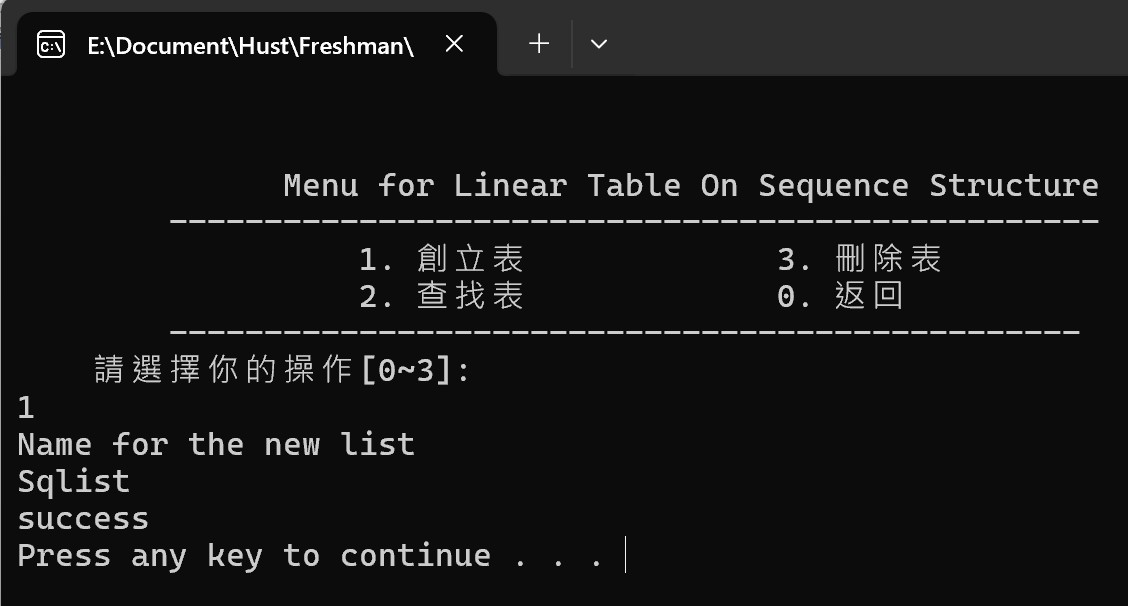
\includegraphics[scale=0.80]{images/1-1.jpg}
		\caption{建立表}
		\label{fig1-1}
	\end{center}
\end{figure}

\subsubsubsection{查找表}
如图所示我们成功地找到了刚刚建立的表"Sqlist"
\begin{figure}[H] % here top bottom
	\begin{center}
		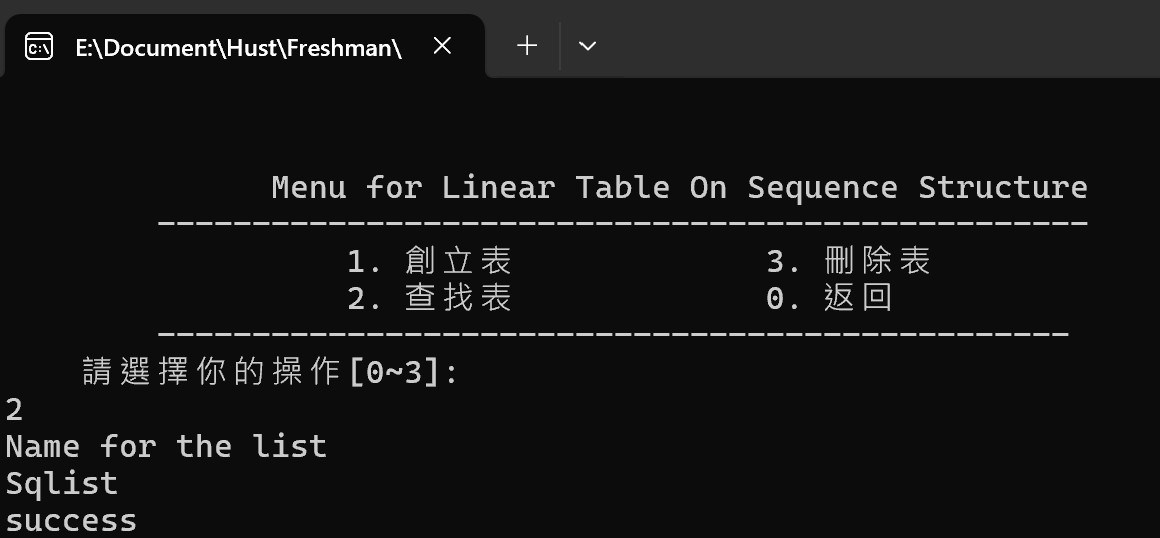
\includegraphics[scale=0.80]{images/1-2.jpg}
		\caption{查找表}
		\label{fig1-2}
	\end{center}
\end{figure}
\subsubsubsection{删除表}
如图所示这里删除失败是因为我们并没有建立名为"abc"的表因此此表不存在找不到表所以删除失败。
\begin{figure}[H] % here top bottom
	\begin{center}
		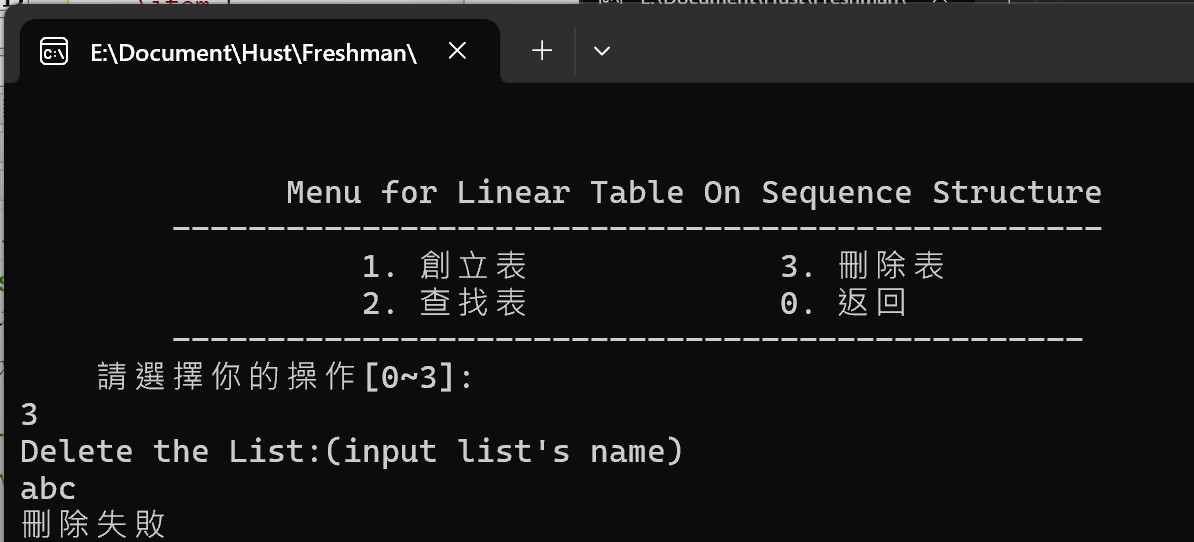
\includegraphics[scale=0.80]{images/1-3.jpg}
		\caption{删除表}
		\label{fig1-3}
	\end{center}
\end{figure}
\subsubsubsection{初始化表}
这里因为多表管理己经建立表Sqlist了，因此initlist时表己存在
\begin{figure}[H] % here top bottom
	\begin{center}
		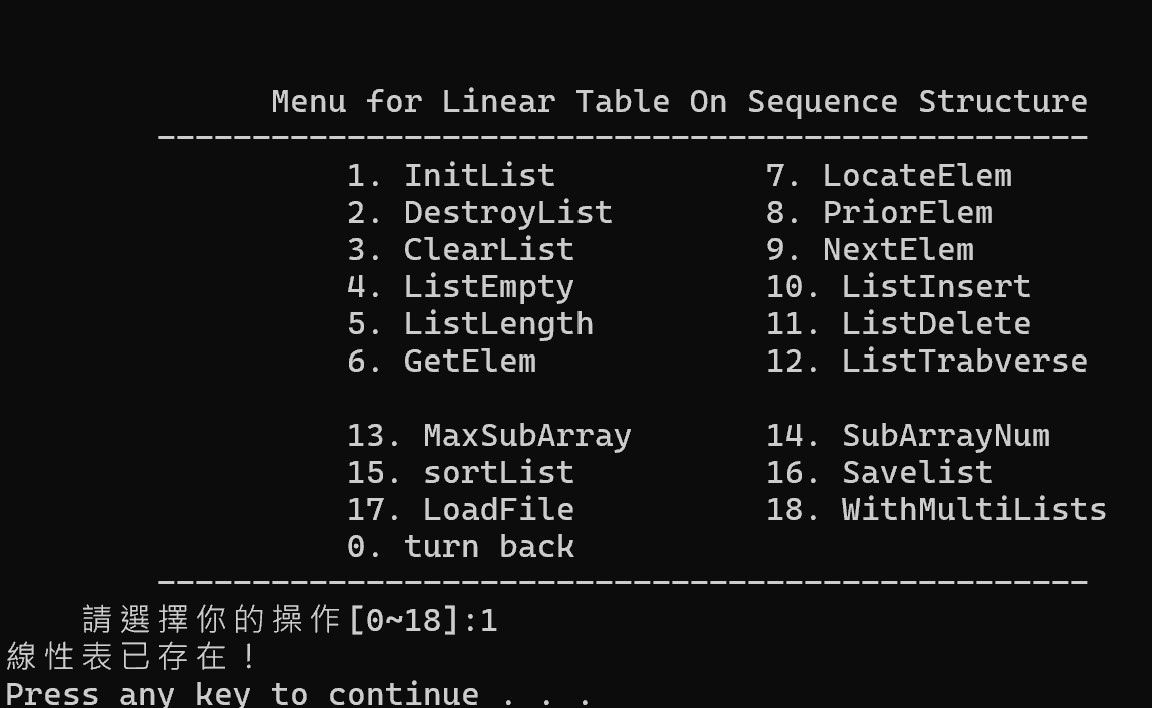
\includegraphics[scale=0.80]{images/1-4.jpg}
		\caption{初始化表}
		\label{fig1-4}
	\end{center}
\end{figure}

\subsubsubsection{判空表}
这里我们判断表是否为空，目前因为没有输入任何的数据内容因此表为空
\begin{figure}[H] % here top bottom
	\begin{center}
		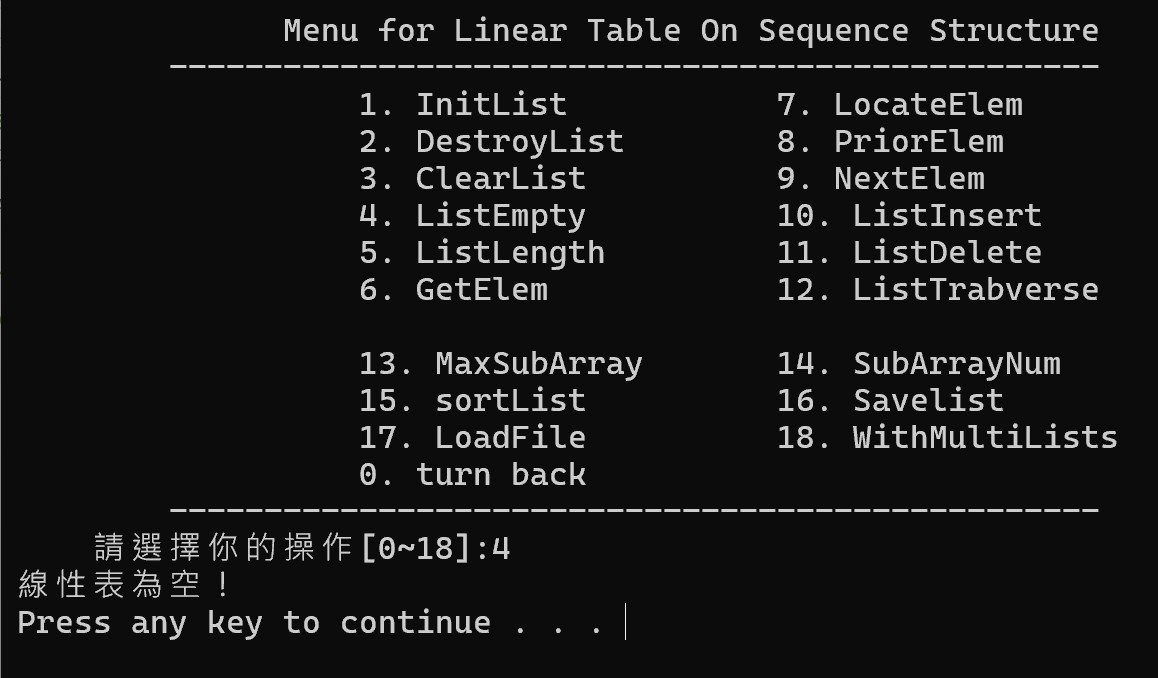
\includegraphics[scale=0.80]{images/1-5.jpg}
		\caption{判空表}
		\label{fig1-5}
	\end{center}
\end{figure}
\subsubsubsection{插入元素}
这里我们在表中插入一个元素5
\begin{figure}[H] % here top bottom
	\begin{center}
		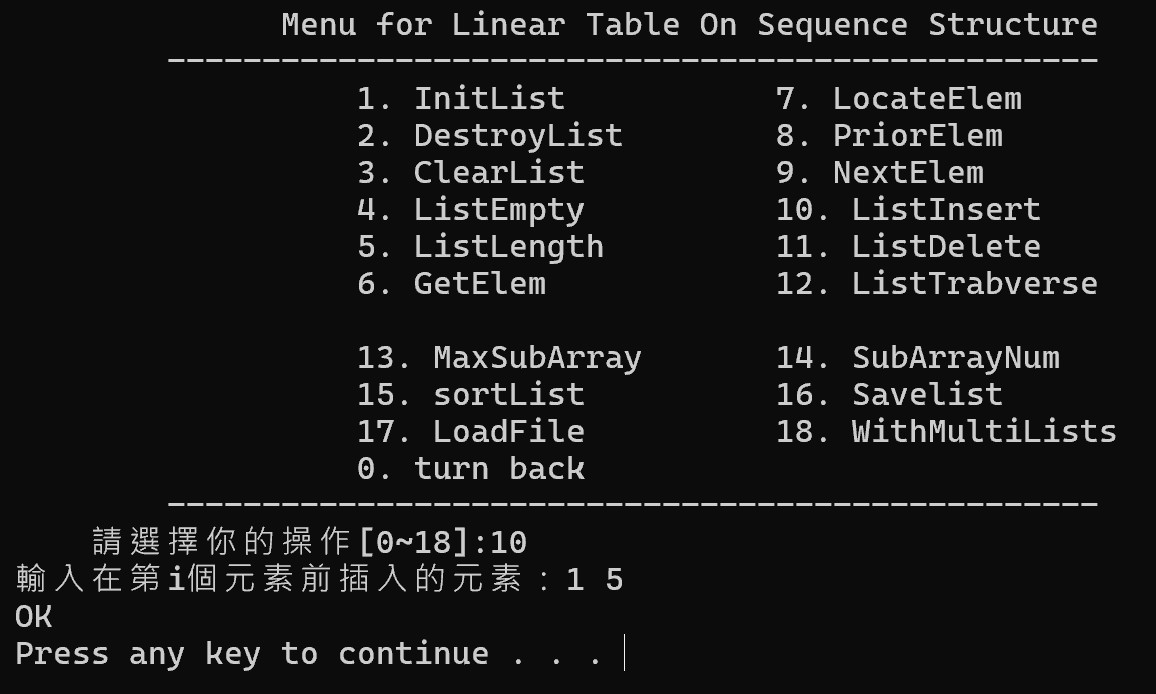
\includegraphics[scale=0.80]{images/1-6.jpg}
		\caption{插入元素}
		\label{fig1-6}
	\end{center}
\end{figure}
\subsubsubsection{查表长}
因为目前表中只有元素5，一个元素因此长度为1
\begin{figure}[H] % here top bottom
	\begin{center}
		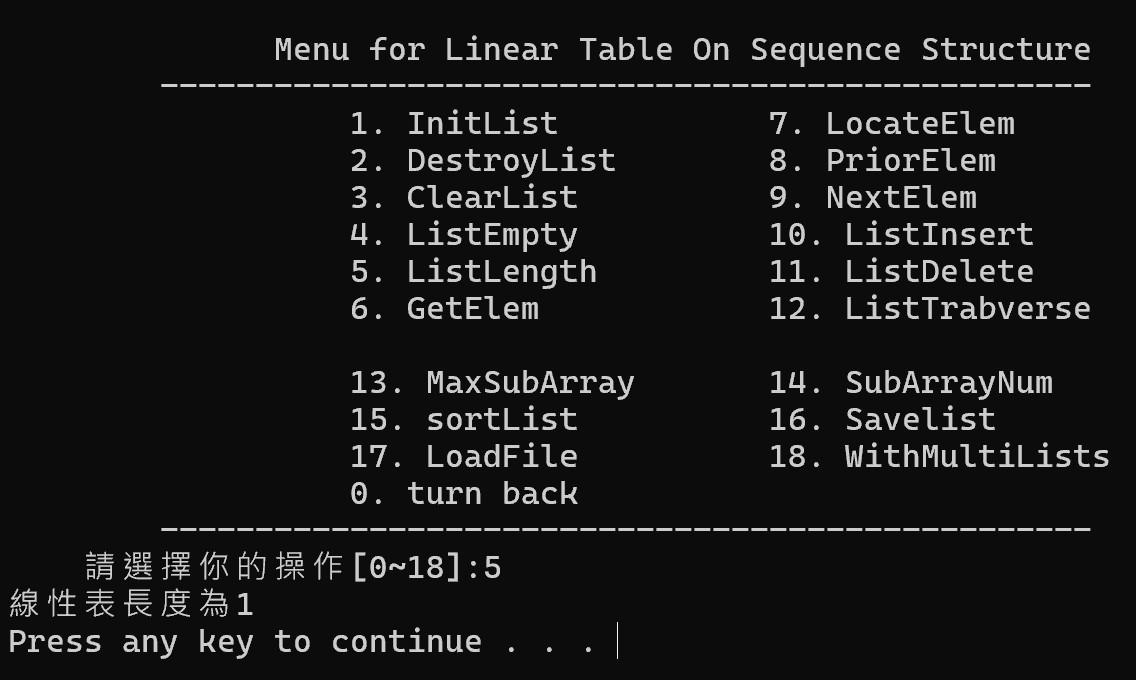
\includegraphics[scale=0.80]{images/1-7.jpg}
		\caption{查表长}
		\label{fig1-7}
	\end{center}
\end{figure}
\subsubsubsection{找特定元素}
\begin{figure}[H] % here top bottom
	\begin{center}
		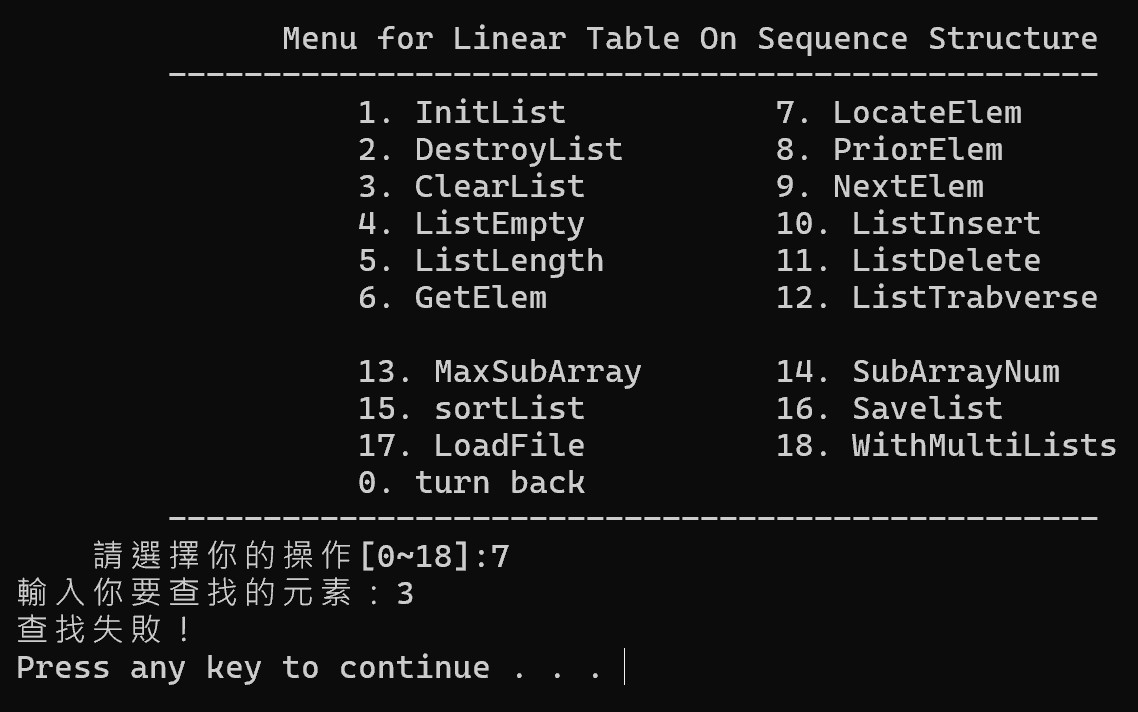
\includegraphics[scale=0.80]{images/1-8.jpg}
		\caption{找特定元素}
		\label{fig1-8}
	\end{center}
\end{figure}
\subsubsubsection{遍历表}
只里我们插入元素5 3 4 2，然后遍历一下看看能否顺利输出
\begin{figure}[H] % here top bottom
	\begin{center}
		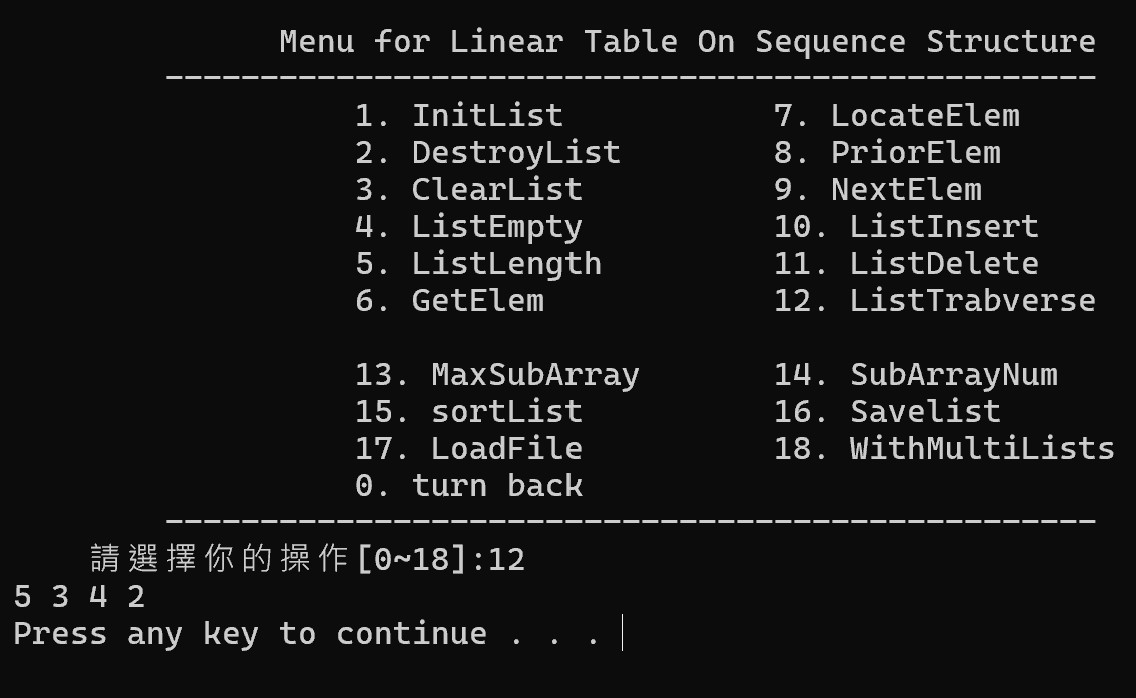
\includegraphics[scale=0.80]{images/1-9.jpg}
		\caption{遍历表}
		\label{fig1-9}
	\end{center}
\end{figure}
\subsubsubsection{查找前驱}
这里数列仍为5 3 4 2，我们找3的前驱看不是5。
\begin{figure}[H] % here top bottom
	\begin{center}
		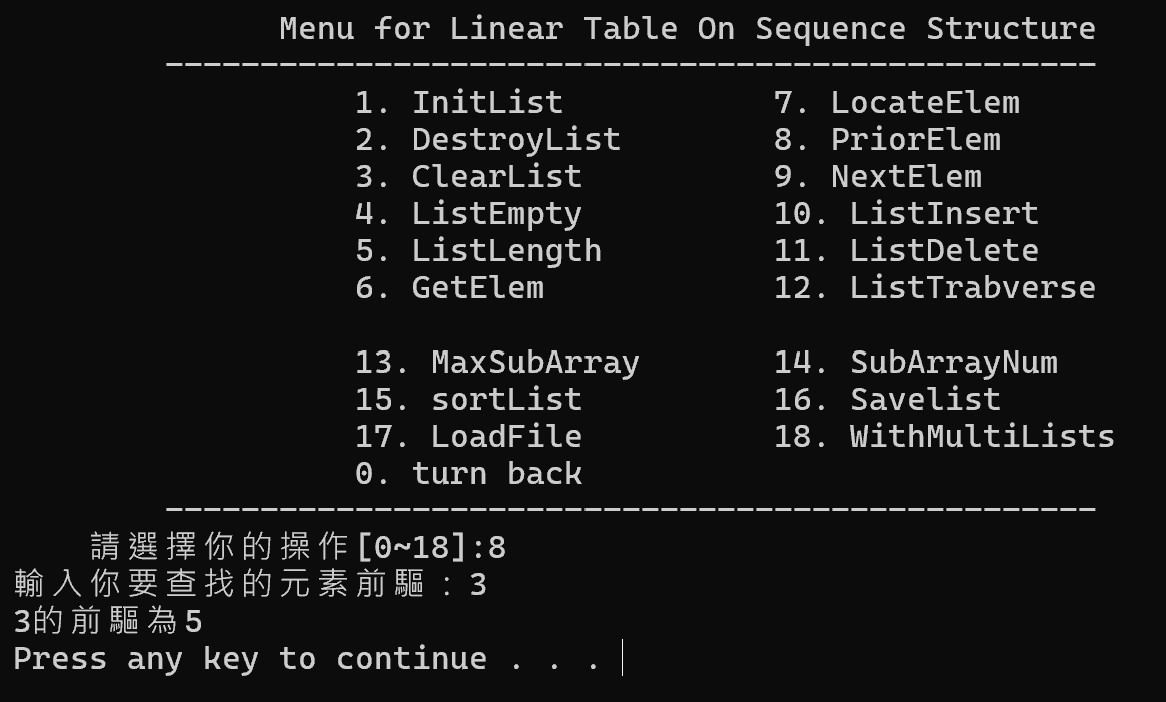
\includegraphics[scale=0.80]{images/1-10.jpg}
		\caption{查找前驱}
		\label{fig1-10}
	\end{center}
\end{figure}
\subsubsubsection{查找后驱}
这里数列仍为5 3 4 2，我们找3的后驱看不是4。
\begin{figure}[H] % here top bottom
	\begin{center}
		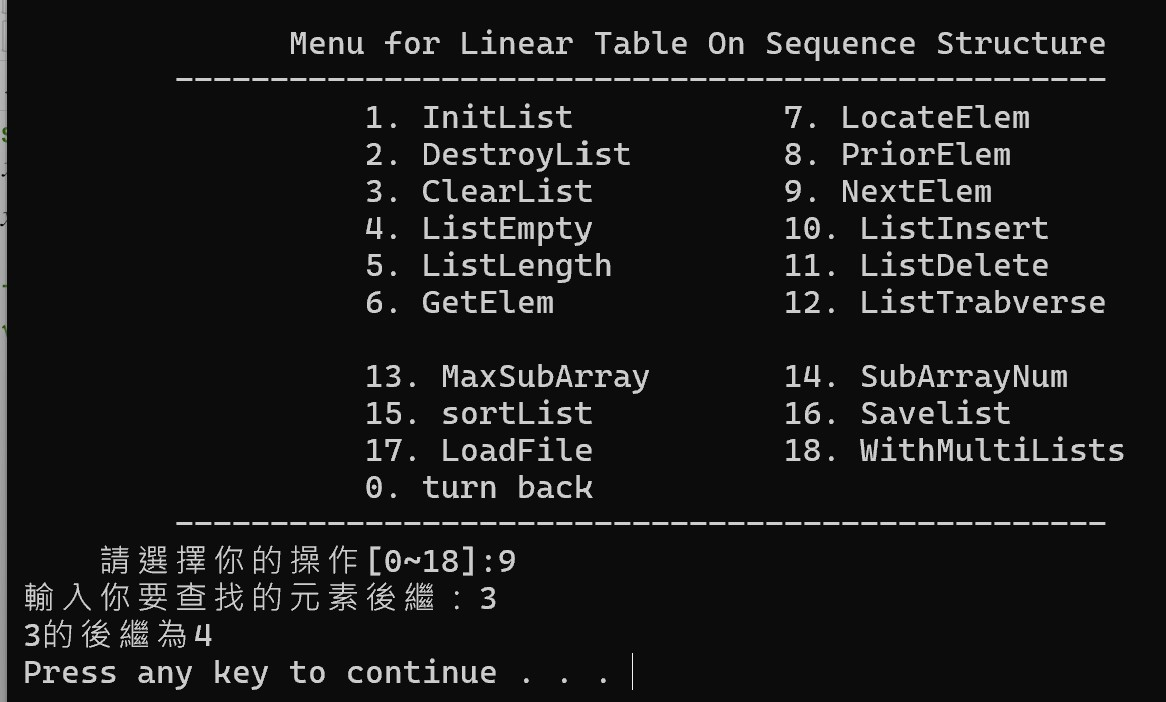
\includegraphics[scale=0.80]{images/1-11.jpg}
		\caption{查找后驱}
		\label{fig1-11}
	\end{center}
\end{figure}
\subsubsubsection{删除元素}
这里我们试一下删除5号位的元素，但我们知道5号位没有元素因为不会成功删除
\begin{figure}[H] % here top bottom
	\begin{center}
		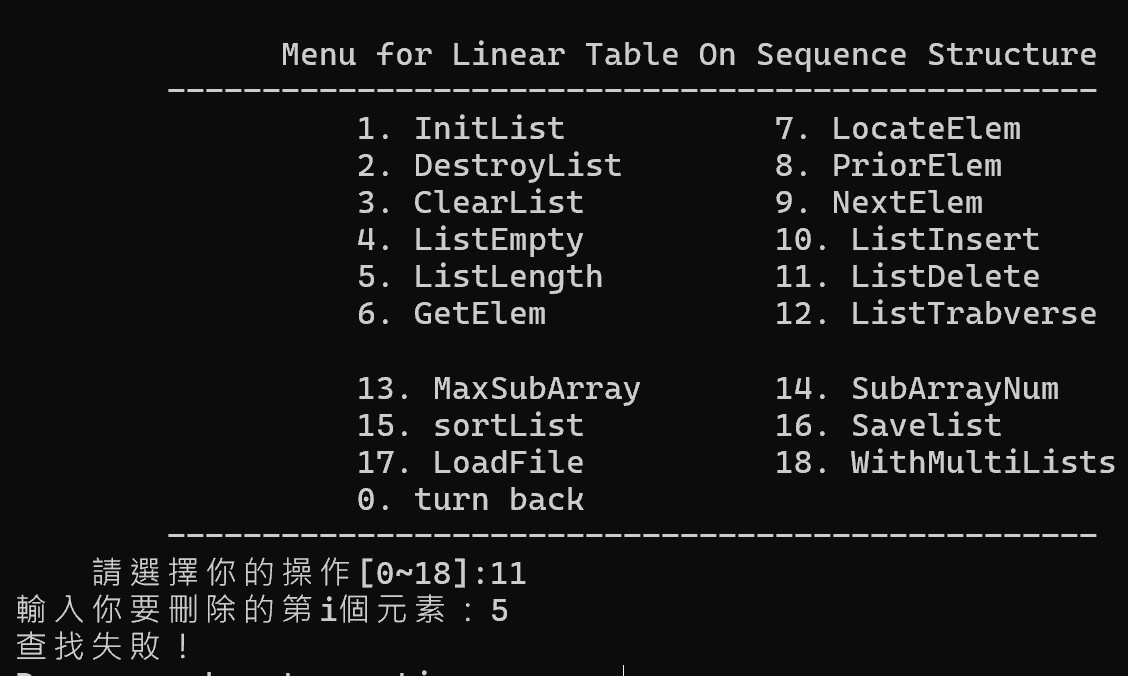
\includegraphics[scale=0.80]{images/1-12.jpg}
		\caption{初始化表}
		\label{fig1-12}
	\end{center}
\end{figure}
\subsubsubsection{排序表}
我们把数列5 3 4 2排序一下看是不是顺利排成2 3 4 5
\begin{figure}[H] % here top bottom
	\begin{center}
		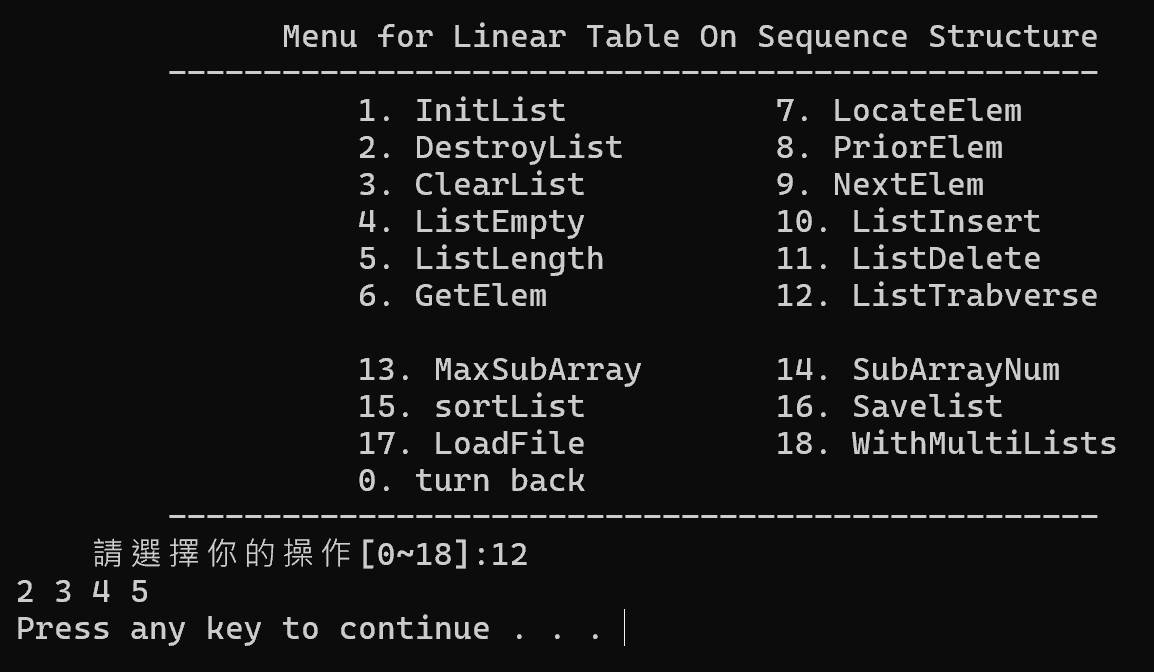
\includegraphics[scale=0.80]{images/1-13.jpg}
		\caption{排序表}
		\label{fig1-13}
	\end{center}
\end{figure}
\subsubsubsection{存取表}
这里我们先保存为sqlist1.txt然后清空表再加载一下看能不能找回来，我们发现是可以加载回来的啊，仍然是2 3 4 5
\begin{figure}[H] % here top bottom
	\begin{center}
		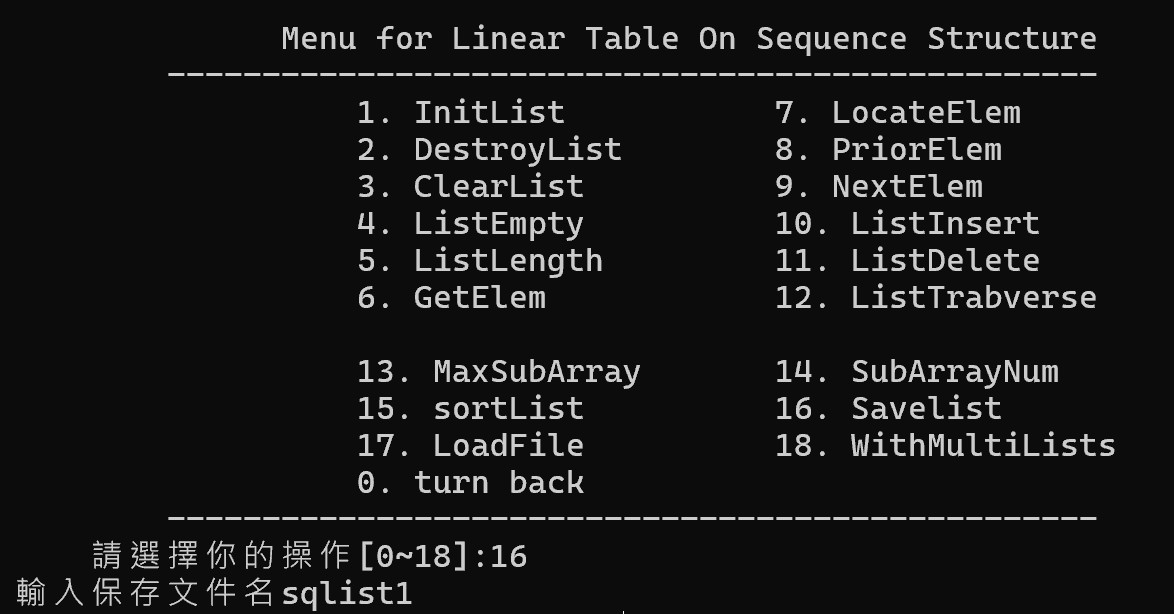
\includegraphics[scale=0.80]{images/1-14.jpg}
		\caption{保存表}
		\label{fig1-14}
	\end{center}
\end{figure}
\begin{figure}[H] % here top bottom
	\begin{center}
		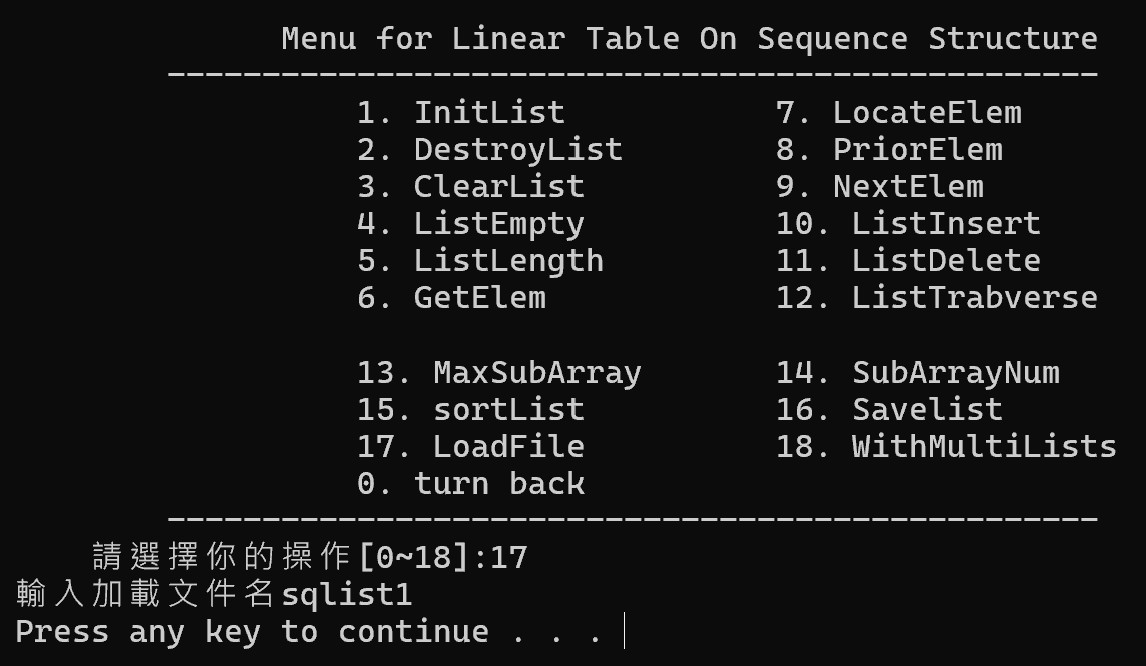
\includegraphics[scale=0.80]{images/1-15.jpg}
		\caption{加载表}
		\label{fig1-15}
	\end{center}
\end{figure}
\begin{figure}[H] % here top bottom
	\begin{center}
		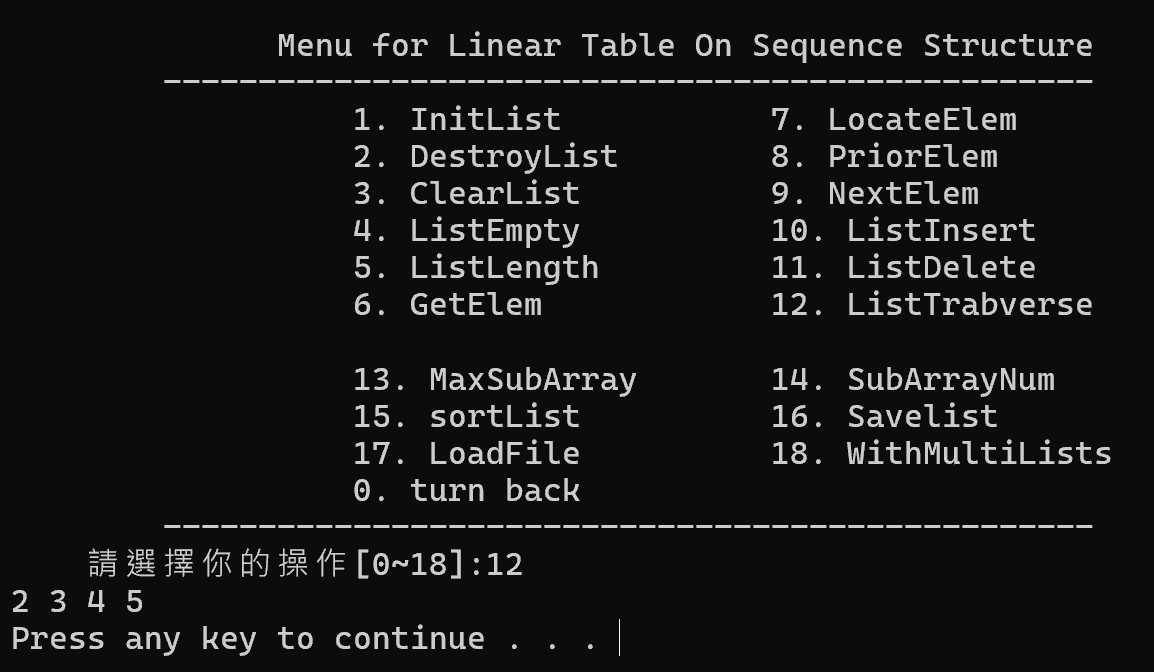
\includegraphics[scale=0.80]{images/1-16.jpg}
		\caption{遍历表}
		\label{fig1-16}
	\end{center}
\end{figure}
\subsubsubsection{最大连续子数组和}
我们看看最大连续子数组和是不是2+3+4+5=14
\begin{figure}[H] % here top bottom
	\begin{center}
		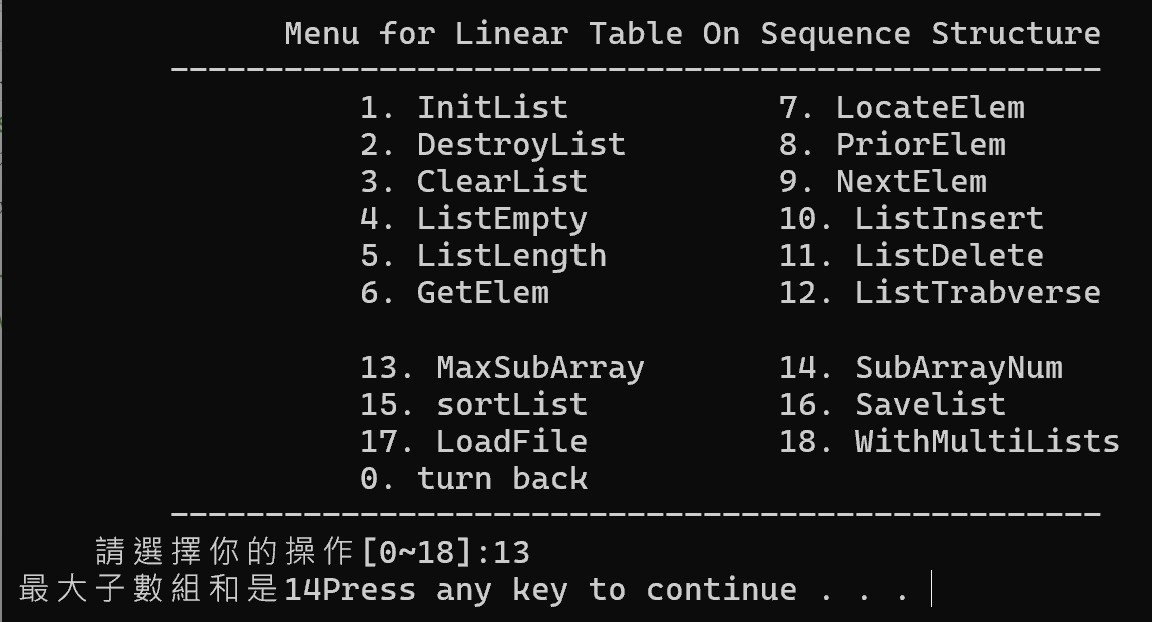
\includegraphics[scale=0.80]{images/1-17.jpg}
		\caption{最大连续子数组和}
		\label{fig1-17}
	\end{center}
\end{figure}
\subsubsubsection{和为K的子数组}
我们输入7看看是不是能够找剽3+4=7这对数组
\begin{figure}[H] % here top bottom
	\begin{center}
		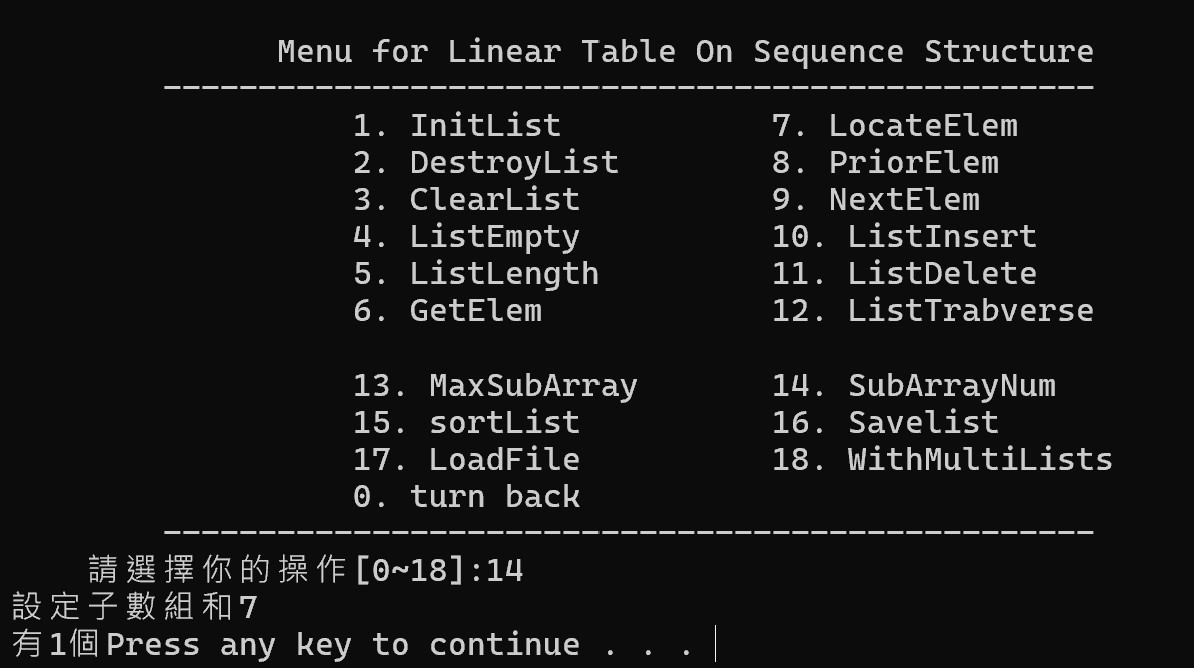
\includegraphics[scale=0.80]{images/1-18.jpg}
		\caption{和为K的子数组}
		\label{fig1-18}
	\end{center}
\end{figure}

至此，我们可以说是成功测试了程序的基本要求了，实现了顺序表的多表管理和基本运算要求。
\subsection{实验小结}

在本次 C 语言实现顺序表多表管理的实验中，我成功完成了对多个顺序表的创建、插入、删除、查找及遍历等核心操作。通过将理论知识转化为实践代码，我不仅加深了对顺序表数据结构特性的理解，也掌握了如何通过动态内存分配灵活管理多个顺序表的存储与操作。\\
在实验过程中，我采用结构体数组存储多个顺序表的表头信息，每个表头结构体包含了顺序表的容量、当前长度以及数据元素数组指针。这种设计方式有效实现了对多个顺序表的统一管理，同时也通过模块化编程，将每个功能封装为独立函数，增强了代码的可读性与可维护性。例如，在插入元素的函数实现中，我充分考虑了顺序表满时的动态扩容操作，确保了数据插入的可靠性；而在删除元素函数里，则通过合理的元素移动策略，维持了顺序表数据的连续性。

\newpage

\section{基于邻接表的图实现}

\subsection{实验目的}
通过实验达到：
\begin{enumerate}
	\item	加深对图的概念、基本运算的理解
	\item	熟练掌握图的逻辑结构与物理结构的关系
	\item	以邻接表作为物理结构，熟练掌握图基本运算的实现。
\end{enumerate}

\subsection{邻接表的图基本運算}
\begin{enumerate}
	\item	创建图：函数名称是CreateCraph(G,V,V0,9R)；初始条件是V是图的顶点集，VR是图的关系集；操作结果是按V和VR的定义构造图G；
	注：①要求图G中顶点关键字具有唯一性。后面各操作的实现，也都要满足一个图中关键字的唯一性，不再赘述；② V和VR对应的是图的逻辑定义形式，比如V为顶点序列，VR为关键字对的序列。不能将邻接矩阵等物理结构来代替V和VR。
	\item	销毁图：函数名称是DestroyGraph(G)；初始条件图G已存在；操作结果是销毁图G；
	\item	查找顶点：函数名称是LocateVex(G,u)；初始条件是图G存在，u是和G中顶点关键字类型相同的给定值；操作结果是若u在图G中存在，返回关键字为u的顶点位置序号（简称位序），否则返回其它表示“不存在”的信息；
	\item	顶点赋值：函数名称是PutVex (G,u,value)；初始条件是图G存在，u是和G中顶点关键字类型相同的给定值；操作结果是对关键字为u的顶点赋值value；
	\item	获得第一邻接点：函数名称是FirstAdjVex(G, u)；初始条件是图G存在，u是G中顶点的位序；操作结果是返回u对应顶点的第一个邻接顶点位序，如果u的顶点没有邻接顶点，否则返回其它表示“不存在”的信息；
	\item	获得下一邻接点：函数名称是NextAdjVex(G, v, w)；初始条件是图G存在，v和w是G中两个顶点的位序，v对应G的一个顶点,w对应v的邻接顶点；操作结果是返回v的（相对于w）下一个邻接顶点的位序，如果w是最后一个邻接顶点，返回其它表示“不存在”的信息；
	\item	插入顶点：函数名称是InsertVex(G,v)；初始条件是图G存在，v和G中的顶点具有相同特征；操作结果是在图G中增加新顶点v。（在这里也保持顶点关键字的唯一性）；
	\item	删除顶点：函数名称是DeleteVex(G,v)；初始条件是图G存在，v是和G中顶点关键字类型相同的给定值；操作结果是在图G中删除关键字v对应的顶点以及相关的弧；
	\item	插入弧：函数名称是InsertArc(G,v,w)；初始条件是图G存在，v、w是和G中顶点关键字类型相同的给定值；操作结果是在图G中增加弧<v,w>，如果图G是无向图，还需要增加<w,v>；
	\item	删除弧：函数名称是DeleteArc(G,v,w)；初始条件是图G存在，v、w是和G中顶点关键字类型相同的给定值；操作结果是在图G中删除弧<v,w>，如果图G是无向图，还需要删除<w,v>；
	\item	深度优先搜索遍历：函数名称是DFSTraverse(G,visit())；初始条件是图G存在；操作结果是图G进行深度优先搜索遍历，依次对图中的每一个顶点使用函数visit访问一次，且仅访问一次；
	\item	广度优先搜索遍历：函数名称是BFSTraverse(G,visit())；初始条件是图G存在；操作结果是图G进行广度优先搜索遍历，依次对图中的每一个顶点使用函数visit访问一次，且仅访问一次。
\end{enumerate}
\begin{enumerate}
	\item 	附加功能：
	\item	距离小于k的顶点集合：函数名称是VerticesSetLessThanK(G,v,k)，初始条件是图G存在；操作结果是返回与顶点v距离小于k的顶点集合；
	\item	顶点间最短路径和长度：函数名称是ShortestPathLength(G,v,w); 初始条件是图G存在；操作结果是返回顶点v与顶点w的最短路径的长度；
	\item	图的连通分量：函数名称是ConnectedComponentsNums(G)，初始条件是图G存在；操作结果是返回图G的所有连通分量的个数；
	\item	实现图的文件形式保存：其中，①需要设计文件数据记录格式，以高效保存图的数据逻辑结构(D,{R})的完整信息；②需要设计图文件保存和加载操作合理模式。附录B提供了文件存取的方法；
	\item	实现多个图管理：设计相应的数据结构管理多个图的查找、添加、移除等功能。\\
	*注：附加功能（5）实现多个图管理应能创建、添加、移除多个图，单图和多图的区别仅仅在于图管理的个数不同，多图管理应可自由切换到管理的每个图，并可单独对某图进行单图的所有操作。
\end{enumerate}

\subsection{问题描述}

图的集合G 是由集合V 和集合E 组成，即G=V,E，V 表示图中所有顶点的集合，E 表示顶点之间所有边的集合。\\
图是一种数据结构，加上一组基本操作，就成了抽象数据类型。依据最小完备性和常用性相结合的原则，以函数形式定义了创建图、销毁图、查找顶点、获得顶点值和顶点赋值等12 种基本运算。即，我们利用邻接表的形式，完成对图的数据结构的实现。而在本次实验中，我们假定设计的图皆为无向图。

\subsection{系统设计}
首先为在C语言下实现上述功能，我们大致可以分为三个部分，主程序框架、多图管理框架菜单、对当前图操作框架菜单\\主程序框架负责实现多图管理和对当前图操作的框架切换和退出终止的操作。\\
而多图管理则是负责多个图的读写操作，那么则需是编号或命名等操作去区分不同的图，因此我们需要设计一个struct结构去装下这些信息。\\
而最后一个对当前图操作则是对传入的图去进行图的基本运算等操作，负责装下这些函数和选择调用。

\subsection{系统实现}

在设计这么一个菜单框架时我们可以通过多种的方法去实现，那么我的方法是通过switch()函数和goto语法实现在多个switch-while框架中的切换，除此之外我们也可以通过函数指针去实现此菜单功能，然后利用system("PAUSE"); 实现了消除了每次操作后的「清屏」，使得菜单功能选项仍然出现在屏上不需改变位置。\\随后的则是建立多表操作如建立表，删除表，查找并选择表，返回主菜单判断是要继续对表操作还是终止操作，即对此表操作。\\
而在当前表操作时则是在加入多个基本运算之外还要加一个返回主菜单操作。\\
\subsubsection{创建图}
\subsubsubsection{函数基本说明}
函数名称是CreateCraph(G,V,V0,9R)；初始条件是V是图的顶点集，VR是图的关系集；操作结果是按V和VR的定义构造图G；\\
注：①要求图G中顶点关键字具有唯一性。后面各操作的实现，也都要满足一个图中关键字的唯一性，不再赘述；② V和VR对应的是图的逻辑定义形式，比如V为顶点序列，VR为关键字对的序列。不能将邻接矩阵等物理结构来代替V和VR。(\ref{lst:2-1})；
\begin{lstlisting}[style=commonCodeStyle, caption={目标程序}, label={lst:2-1}]
	#include<map>
	std::map<int,int> flag;
	int LocateVex(ALGraph &G, KeyType key) {
		for (int i = 0; i < G.vexnum; ++i) {
			if (G.vertices[i].data.key == key)
			return i;
		}
		return -1;
	}
	status CreateCraph(ALGraph &G,VertexType V[],KeyType VR[][2])
	{
		G.vexnum = 0;
		while (G.vexnum <= MAX_VERTEX_NUM && V[G.vexnum].key != -1) { // 假设以-1结束
			G.vexnum++;
		}
		if (G.vexnum > MAX_VERTEX_NUM or G.vexnum==0) return ERROR;
		for (int i = 0; i < G.vexnum; ++i) {
			for (int j = i + 1; j < G.vexnum; ++j) {
				if (V[i].key == V[j].key)
				return ERROR;
			}
		}
		for (int i = 0; i < G.vexnum; ++i) {
			G.vertices[i].data = V[i];
			G.vertices[i].firstarc = NULL;
		}
		G.arcnum = 0;
		while (VR[G.arcnum][0] != -1 && VR[G.arcnum][1] != -1) { // 假设以-1结束
			G.arcnum++;
		}
		for (int k = 0; k < G.arcnum; ++k) {
			KeyType u = VR[k][0];
			KeyType v = VR[k][1];
			
			int i = LocateVex(G, u);
			int j = LocateVex(G, v);
			if (i == -1 || j == -1)
			return ERROR;
			
			// 将j添加到i的邻接表中
			ArcNode *arc_i = (ArcNode *)malloc(sizeof(ArcNode));
			if (!arc_i) return OVERFLOW;
			arc_i->adjvex = j;
			arc_i->nextarc = G.vertices[i].firstarc;
			G.vertices[i].firstarc = arc_i;
			
			// 将i添加到j的邻接表中
			ArcNode *arc_j = (ArcNode *)malloc(sizeof(ArcNode));
			if (!arc_j) {
				free(arc_i);
				return OVERFLOW;
			}
			arc_j->adjvex = i;
			arc_j->nextarc = G.vertices[j].firstarc;
			G.vertices[j].firstarc = arc_j;
		}
		G.kind = UDG;
		return OK;
	}
	
\end{lstlisting}
\subsubsection{销毁图}
\subsubsubsection{函数基本说明}
函数名称是DestroyGraph(G)；初始条件图G已存在；操作结果是销毁图G；(\ref{lst:2-2})；
\begin{lstlisting}[style=commonCodeStyle, caption={目标程序}, label={lst:2-2}]
	status DestroyGraph(ALGraph &G)
	{
		for (int i = 0; i < G.vexnum; i++) 
		{ 
			ArcNode *p = G.vertices[i].firstarc; 
			while (p) 
			{ 
				ArcNode *q = p; 
				p = p->nextarc; 
				free(q); 
			} 
			G.vertices[i].firstarc = NULL; 
		} 
		G.vexnum = 0; 
		G.arcnum = 0; 
		return OK; 
	}
	
\end{lstlisting}
\subsubsection{查找顶点}
\subsubsubsection{函数基本说明}
函数名称是LocateVex(G,u)；初始条件是图G存在，u是和G中顶点关键字类型相同的给定值；操作结果是若u在图G中存在，返回关键字为u的顶点位置序号（简称位序），否则返回其它表示“不存在”的信息；(\ref{lst:2-3})；
\begin{lstlisting}[style=commonCodeStyle, caption={目标程序}, label={lst:2-3}]
	int LocateVex(ALGraph G,KeyType u)
	
	for (int i = 0; i < G.vexnum; ++i) {
		if(G.vertices[i].data.key == u) return i;
	}
	return -1;
}

\end{lstlisting}
\subsubsection{顶点赋值}
\subsubsubsection{函数基本说明}
函数名称是PutVex (G,u,value)；初始条件是图G存在，u是和G中顶点关键字类型相同的给定值；操作结果是对关键字为u的顶点赋值value；(\ref{lst:2-4})；
\begin{lstlisting}[style=commonCodeStyle, caption={目标程序}, label={lst:2-4}]
int check(ALGraph G,int x,VertexType v){
	for (int i = 0; i < G.vexnum; ++i) {
		if(i == x) continue ;
		if(v.key == G.vertices[i].data.key) return 0;
	}
	return 1;    
}
status PutVex(ALGraph &G,KeyType u,VertexType value)
{
	for (int i = 0; i < G.vexnum; ++i) {
		if(G.vertices[i].data.key == u){
			if(check(G,i,value)== 1){
				G.vertices[i].data=value;
				return OK;
			}
			else return ERROR;
		}
	}
	return ERROR;
}
\end{lstlisting}
\subsubsection{获得第一邻接点}
\subsubsubsection{函数基本说明}
函数名称是FirstAdjVex(G,u)；初始条件是图G存在，u是G中顶点的位序；操作结果是返回u对应顶点的第一个邻接顶点位序，如果u的顶点没有邻接顶点，否则返回其它表示“不存在”的信息；(\ref{lst:2-5})；
\begin{lstlisting}[style=commonCodeStyle, caption={目标程序}, label={lst:2-5}]
int LocateVex(ALGraph G,KeyType u)
{
	for (int i = 0; i < G.vexnum; ++i) {
		if(G.vertices[i].data.key == u) return i;
	}
	return -1;
}
int FirstAdjVex(ALGraph G,KeyType u)
//根据u在图G中查找顶点，查找成功返回顶点u的第一邻接顶点位序，否则返回-1；
{
	int t = LocateVex(G,u);
	if(G.vertices[t].firstarc!=NULL) return G.vertices[t].firstarc->adjvex;
	return -1;
}

\end{lstlisting}
\subsubsection{获得下一邻接点}
\subsubsubsection{函数基本说明}
函数名称是NextAdjVex(G, v, w)；初始条件是图G存在，v和w是G中两个顶点的位序，v对应G的一个顶点,w对应v的邻接顶点；操作结果是返回v的（相对于w）下一个邻接顶点的位序，如果w是最后一个邻接顶点，返回其它表示“不存在”的信息；(\ref{lst:2-6})；
\begin{lstlisting}[style=commonCodeStyle, caption={目标程序}, label={lst:2-6}]
int LocateVex(ALGraph G,KeyType u)
{
	for (int i = 0; i < G.vexnum; ++i) {
		if(G.vertices[i].data.key == u) return i;
	}
	return -1;
}
int NextAdjVex(ALGraph G,KeyType v,KeyType w)
{
	int t = LocateVex(G,v);
	int wt = LocateVex(G,w);
	if (t==-1 or wt == -1) return -1;
	ArcNode *p = G.vertices[t].firstarc;
	while(p!=NULL){
		if(p->adjvex==wt){
			if(p->nextarc!=NULL) return p->nextarc->adjvex;
			else return -1;
		}
		p=p->nextarc;
	}    
	return -1;
}

\end{lstlisting}
\subsubsection{插入顶点}
\subsubsubsection{函数基本说明}
函数名称是InsertVex(G,v)；初始条件是图G存在，v和G中的顶点具有相同特征；操作结果是在图G中增加新顶点v。（在这里也保持顶点关键字的唯一性）(\ref{lst:2-7})；
\begin{lstlisting}[style=commonCodeStyle, caption={目标程序}, label={lst:2-7}]
status InsertVex(ALGraph &G,VertexType v)
{
	if(G.vexnum == MAX_VERTEX_NUM) return ERROR;
	for(int i=0;i<G.vexnum;i++){
		if(G.vertices[i].data.key==v.key) return ERROR;
	}
	G.vertices[G.vexnum].data = v;
	G.vertices[G.vexnum].firstarc=NULL;
	G.vexnum++;
	return OK;
}

\end{lstlisting}
\subsubsection{删除顶点}
\subsubsubsection{函数基本说明}
函数名称是DeleteVex(G,v)；初始条件是图G存在，v是和G中顶点关键字类型相同的给定值；操作结果是在图G中删除关键字v对应的顶点以及相关的弧；(\ref{lst:2-8})；
\begin{lstlisting}[style=commonCodeStyle, caption={目标程序}, label={lst:2-8}]
int LocateVex(ALGraph G,KeyType u)
{
	for (int i = 0; i < G.vexnum; ++i) {
		if(G.vertices[i].data.key == u) return i;
	}
	return -1;
}
status DeleteVex(ALGraph &G,KeyType v)
{
	if(G.vexnum == 1) return ERROR;
	int pos_v = LocateVex(G, v);
	if (pos_v == -1) return ERROR;
	
	ArcNode *current = G.vertices[pos_v].firstarc;
	while (current != NULL) {
		int w_pos = current->adjvex;
		
		ArcNode *w_prev = NULL;
		ArcNode *w_p = G.vertices[w_pos].firstarc;
		while (w_p != NULL) {
			if (w_p->adjvex == pos_v) {
				if (w_prev == NULL) {
					G.vertices[w_pos].firstarc = w_p->nextarc;
				} else {
					w_prev->nextarc = w_p->nextarc;
				}
				ArcNode *temp = w_p;
				w_p = w_p->nextarc;
				free(temp);
				G.arcnum--; 
				break;
			} else {
				w_prev = w_p;
				w_p = w_p->nextarc;
			}
		}
		ArcNode *temp = current;
		current = current->nextarc;
		free(temp);
	}
	G.vertices[pos_v].firstarc = NULL;
	
	for (int i = pos_v; i < G.vexnum - 1; i++) {
		G.vertices[i] = G.vertices[i + 1];
	}
	G.vexnum--;
	for (int i = 0; i < G.vexnum; i++) {
		ArcNode *p = G.vertices[i].firstarc;
		while (p != NULL) {
			if (p->adjvex > pos_v) {
				p->adjvex--; 
			}
			p = p->nextarc;
		}
	}
	return OK;
}
\end{lstlisting}
\subsubsection{插入弧}
\subsubsubsection{函数基本说明}
函数名称是InsertArc(G,v,w)；初始条件是图G存在，v、w是和G中顶点关键字类型相同的给定值；操作结果是在图G中增加弧<v,w>，如果图G是无向图，还需要增加<w,v>；(\ref{lst:2-9})；
\begin{lstlisting}[style=commonCodeStyle, caption={目标程序}, label={lst:2-9}]
int LocateVex(ALGraph G,KeyType u)
{
	for (int i = 0; i < G.vexnum; ++i) {
		if(G.vertices[i].data.key == u) return i;
	}
	return -1;
}
status InsertArc(ALGraph &G,KeyType v,KeyType w)
{
	int vt = LocateVex(G,v),wt = LocateVex(G,w);
	if(vt == -1 or wt == -1) return ERROR;
	ArcNode *p = G.vertices[wt].firstarc;
	while(p!=NULL){
		if(p->adjvex == vt) return ERROR;
		p=p->nextarc;
	}
	ArcNode *temp1 = (ArcNode *)malloc(sizeof(ArcNode));
	temp1->nextarc = G.vertices[vt].firstarc;
	temp1->adjvex = wt;
	G.vertices[vt].firstarc = temp1;
	ArcNode *temp2 = (ArcNode *)malloc(sizeof(ArcNode));
	temp2->nextarc = G.vertices[wt].firstarc;
	temp2->adjvex = vt;
	G.vertices[wt].firstarc = temp2;    
	G.arcnum++;
	return OK;
}
\end{lstlisting}
\subsubsection{删除弧}
\subsubsubsection{函数基本说明}
函数名称是DeleteArc(G,v,w)；初始条件是图G存在，v、w是和G中顶点关键字类型相同的给定值；操作结果是在图G中删除弧<v,w>，如果图G是无向图，还需要删除<w,v>；(\ref{lst:2-10})；
\begin{lstlisting}[style=commonCodeStyle, caption={目标程序}, label={lst:2-10}]
int LocateVex(ALGraph G,KeyType u)
{
	for (int i = 0; i < G.vexnum; ++i) {
		if(G.vertices[i].data.key == u) return i;
	}
	return -1;
}
status DeleteArc(ALGraph &G,KeyType v,KeyType w)
{
	int v_pos = LocateVex(G, v);
	int w_pos = LocateVex(G, w);
	if (v_pos == -1 || w_pos == -1) return ERROR;
	ArcNode *prev = NULL;
	ArcNode *curr = G.vertices[v_pos].firstarc;
	bool found = false;
	while (curr != NULL) {
		if (curr->adjvex == w_pos) {
			if (prev == NULL) {
				G.vertices[v_pos].firstarc = curr->nextarc;
			} else {
				prev->nextarc = curr->nextarc;
			}
			free(curr);
			found = true;
			break;
		}
		prev = curr;
		curr = curr->nextarc;
	}
	if (!found) return ERROR; 
	prev = NULL;
	curr = G.vertices[w_pos].firstarc;
	while (curr != NULL) {
		if (curr->adjvex == v_pos) {
			if (prev == NULL) {
				G.vertices[w_pos].firstarc = curr->nextarc;
			} else {
				prev->nextarc = curr->nextarc;
			}
			free(curr);
			break;
		}
		prev = curr;
		curr = curr->nextarc;
	}
	G.arcnum--; 
	return OK;
}
\end{lstlisting}
\subsubsection{深度优先搜索遍历}
\subsubsubsection{函数基本说明}
函数名称是DFSTraverse(G,visit())；初始条件是图G存在；操作结果是图G进行深度优先搜索遍历，依次对图中的每一个顶点使用函数visit访问一次，且仅访问一次；(\ref{lst:2-11})；
\begin{lstlisting}[style=commonCodeStyle, caption={目标程序}, label={lst:2-11}]
#include <map>
std::map<int,int> flagdfs;
void dfs(ALGraph G,int t,void (*visit)(VertexType)){
	visit(G.vertices[t].data);
	flagdfs[t]=1;
	ArcNode *p = G.vertices[t].firstarc;
	while(p!=NULL){
		if(flagdfs[p->adjvex]==0) dfs(G,p->adjvex,visit);
		p=p->nextarc;
	}
}
status DFSTraverse(ALGraph &G,void (*visit)(VertexType))
{
	for(int i=0;i<G.vexnum;i++){
		if(flagdfs[i]==0) dfs(G,i,visit);
	}
}
\end{lstlisting}
\subsubsection{广度优先搜索遍历}
\subsubsubsection{函数基本说明}
函数名称是BFSTraverse(G,visit())；初始条件是图G存在；操作结果是图G进行广度优先搜索遍历，依次对图中的每一个顶点使用函数visit访问一次，且仅访问一次。(\ref{lst:2-12})；
\begin{lstlisting}[style=commonCodeStyle, caption={目标程序}, label={lst:2-12}]
#include <map>
#include <queue>
std::map<int,int> flagbfs;
std::queue<int> q;
status BFSTraverse(ALGraph &G,void (*visit)(VertexType))
{
	for(int i=0;i<G.vexnum;i++){
		if(flagbfs[i]==0){
			q.push(i);
			flagbfs[i]=1;
		}
		while(!q.empty()){
			int u=q.front();
			q.pop();
			visit(G.vertices[u].data);
			ArcNode *p = G.vertices[u].firstarc;
			while(p!=NULL){
				if(flagbfs[p->adjvex]==0){
					q.push(p->adjvex);
					flagbfs[p->adjvex]=1;
				}
				p=p->nextarc;
			}
		}
	}
}
\end{lstlisting}
\subsubsection{实现图的文件形式保存}
\subsubsubsection{函数基本说明}
其中，①需要设计文件数据记录格式，以高效保存图的数据逻辑结构(D,{R})的完整信息；②需要设计图文件保存和加载操作合理模式。附录B提供了文件存取的方法；
\\注：①保存到文件后，可以直接加载文件生成图。(\ref{lst:2-13})；
\begin{lstlisting}[style=commonCodeStyle, caption={目标程序}, label={lst:2-13}]
#include<map>
#include <algorithm> 
std::map<int,int> flagsave;
int LocateVex(ALGraph &G, KeyType key) {
	for (int i = 0; i < G.vexnum; ++i) {
		if (G.vertices[i].data.key == key)
		return i;
	}
	return -1;
}
status CreateCraph0(ALGraph &G,VertexType V[],KeyType VR[][2])
{
	G.vexnum = 0;
	while (G.vexnum <= MAX_VERTEX_NUM && V[G.vexnum].key != -1) {
		G.vexnum++;
	}
	if (G.vexnum > MAX_VERTEX_NUM or G.vexnum==0) return ERROR;
	for (int i = 0; i < G.vexnum; ++i) {
		for (int j = i + 1; j < G.vexnum; ++j) {
			if (V[i].key == V[j].key)
			return ERROR;
		}
	}
	for (int i = 0; i < G.vexnum; ++i) {
		G.vertices[i].data = V[i];
		G.vertices[i].firstarc = NULL;
	}
	G.arcnum = 0;
	while (VR[G.arcnum][0] != -1 && VR[G.arcnum][1] != -1) {
		G.arcnum++;
	}
	for (int k = 0; k < G.arcnum; ++k) {
		KeyType u = VR[k][0];
		KeyType v = VR[k][1];
		int i = LocateVex(G, u);
		int j = LocateVex(G, v);
		if (i == -1 || j == -1)
		return ERROR;
		ArcNode *arc_i = (ArcNode *)malloc(sizeof(ArcNode));
		if (!arc_i) return OVERFLOW;
		arc_i->adjvex = j;
		arc_i->nextarc = G.vertices[i].firstarc;
		G.vertices[i].firstarc = arc_i;
		ArcNode *arc_j = (ArcNode *)malloc(sizeof(ArcNode));
		if (!arc_j) {
			free(arc_i);
			return OVERFLOW;
		}
		arc_j->adjvex = i;
		arc_j->nextarc = G.vertices[j].firstarc;
		G.vertices[j].firstarc = arc_j;
	}
	G.kind = UDG;
	return OK;
}

status SaveGraph(ALGraph G, char FileName[])
{
	FILE *fp = fopen(FileName, "w");
	for(int i=0;i<G.vexnum;i++){
		fprintf(fp,"%d %s ", G.vertices[i].data.key , G.vertices[i].data.others); 
	}
	fprintf(fp,"%d %s ", -1 , "nil"); 
	for(int i=0;i<G.vexnum;i++){
		flagsave[i]=1;
		ArcNode *p = G.vertices[i].firstarc;
		while(p!=NULL){
			if(flagsave[p->adjvex] == 0){
				fprintf(fp,"%d %d ", G.vertices[i].data.key , G.vertices[p->adjvex].data.key);                     
			}
			p=p->nextarc; 
		}
	}    
	fprintf(fp,"%d %d ", -1 , -1);
	fclose(fp);
	return OK;
}
status LoadGraph(ALGraph &G, char FileName[])
{
	FILE *fp = fopen(FileName, "r");
	VertexType V[21];
	KeyType VR[100][2];
	int i=0;
	do {
		fscanf(fp,"%d%s",&V[i].key,V[i].others);
	} while(V[i++].key!=-1);
	i=0;
	do {
		fscanf(fp,"%d%d",&VR[i][0],&VR[i][1]);
		if(VR[i][0]>VR[i][1]) std::swap(VR[i][0],VR[i][1]);
	} while(VR[i++][0]!=-1);
	i--;
	for(int j=0;j<i-1;j++){
		for(int r=0;r<i-1-j;r++)
		if(VR[r][0] > VR[r+1][0] || (VR[r][0] == VR[r+1][0] && VR[r][1] > VR[r+1][1])){
			std::swap(VR[r],VR[r+1]);
		}
	}
	if(CreateCraph0(G,V,VR)==OK) {
		fclose(fp);
		return OK;
	}
	else{
		fclose(fp);
		return ERROR;               
	}
}

\end{lstlisting}
\subsubsection{距离小于k的顶点集合}
\subsubsubsection{函数基本说明}
函数名称是VerticesSetLessThanK(G,v,k)，初始条件是图G存在；操作结果是返回与顶点v距离小于k的顶点集合；(\ref{lst:2-14})；
\begin{lstlisting}[style=commonCodeStyle, caption={目标程序}, label={lst:2-14}]
int VerticesSetLessThanK(ALGraph &G,int v,int k){
	int u0= LocateVex(G,v),s[100]={-1};
	if(u0==-1) return ERROR;
	q.push(u0);
	s[u0]=0;
	flagbfs[u0]=1;
	printf("%d %s\n",G.vertices[u0].data.key,G.vertices[u0].data.others);   
	while(!q.empty()){
		int u=q.front();
		q.pop();
		ArcNode *p = G.vertices[u].firstarc;
		while(p!=NULL){
			if(flagbfs[p->adjvex]==0){
				s[p->adjvex]=s[u]+1;
				if(s[p->adjvex]<k){
					flagbfs[p->adjvex]=1;
					q.push(p->adjvex);
					printf("%d %s\n",G.vertices[p->adjvex].data.key,G.vertices[p->adjvex].data.others);                     
				}                               
			}
			p=p->nextarc;
		}
	}
	return OK;
}
\end{lstlisting}
\subsubsection{顶点间最短路径和长度}
\subsubsubsection{函数基本说明}
函数名称是ShortestPathLength(G,v,w); 初始条件是图G存在；操作结果是返回顶点v与顶点w的最短路径的长度；(\ref{lst:2-15})；
\begin{lstlisting}[style=commonCodeStyle, caption={目标程序}, label={lst:2-15}]
int ShortestPathLength(ALGraph &G,int v,int k){
	int u0= LocateVex(G,v),s[100]={-1},v0=LocateVex(G,k);
	if(u0==-1 or v0==-1) return -1;
	q.push(u0);
	s[u0]=0;
	flagbfs[u0]=1;
	while(!q.empty()){
		int u=q.front();
		q.pop();
		ArcNode *p = G.vertices[u].firstarc;
		while(p!=NULL){
			if(flagbfs[p->adjvex]==0){
				s[p->adjvex]=s[u]+1;
				if(p->adjvex==v0){
					return s[p->adjvex];                
				}           
				flagbfs[p->adjvex]=1;
				q.push(p->adjvex);                  
			}
			p=p->nextarc;
		}
	}
	return ERROR;
}
\end{lstlisting}
\subsubsection{图的连通分量}
\subsubsubsection{函数基本说明}
函数名称是ConnectedComponentsNums(G)，初始条件是图G存在；操作结果是返回图G的所有连通分量的个数；(\ref{lst:2-16})；
\begin{lstlisting}[style=commonCodeStyle, caption={目标程序}, label={lst:2-16}]
int ConnectedComponentsNums(ALGraph &G){
	if(G.vexnum==0) return -1;
	int s=0; 
	for(int i=0;i<G.vexnum;i++){
		if(flagbfs[i]==0){
			q.push(i);
			flagbfs[i]=1;
		}
		else continue;
		while(!q.empty()){
			int u=q.front();
			q.pop();
			ArcNode *p = G.vertices[u].firstarc;
			while(p!=NULL){
				if(flagbfs[p->adjvex]==0){
					q.push(p->adjvex);
					flagbfs[p->adjvex]=1;
				}
				p=p->nextarc;
			}
		}
		s++;
	}
	return s;
}
\end{lstlisting}
\subsubsection{实现多个图管理}
\subsubsubsection{函数基本说明}
设计相应的数据结构管理多个图的查找、添加、移除等功能。(\ref{lst:2-17})；
\begin{lstlisting}[style=commonCodeStyle, caption={目标程序}, label={lst:2-17}]
status AddList(LISTS &Lists,char ListName[])
{
	Lists.elem[Lists.length].G = ALGraph(); // C++ 方式初始化
	ALGraph &graph = Lists.elem[Lists.length].G;
	graph.vexnum = 0;
	graph.arcnum = 0;
	graph.kind = UDG;
	for (int i = 0; i < MAX_VERTEX_NUM; i++) {
		graph.vertices[i].firstarc = NULL;
	}
	strcpy(Lists.elem[Lists.length].name,ListName);
	Lists.length++;
	return OK;
}
status RemoveList(LISTS &Lists,char ListName[])
{
	for(int i=0;i<Lists.length;i++){
		if(strcmp(ListName,Lists.elem[i].name)==0){
			for(int j=i;j<Lists.length-1;j++){
				Lists.elem[j]=Lists.elem[j+1];
			}
			Lists.length--;
			return OK;
		}
	}
	return ERROR;
}
int LocateList(LISTS Lists,char ListName[])
{
	for(int i=0;i<Lists.length;i++){
		if(strcmp(Lists.elem[i].name,ListName)==0) return i+1;
	}
	return ERROR;
}
\end{lstlisting}
\subsubsection{初始化表}
\subsubsubsection{函数基本说明}
函数名称是InitList(L)；初始条件是线性表L不存在；操作结果是构造一个空的线性表(\ref{lst:1-1})；
\begin{lstlisting}[style=commonCodeStyle, caption={目标程序}, label={lst:1-1}]
status InitList(SqList& L)
{
	if(L.elem == NULL)
	{
		L.elem=(ElemType *) malloc(sizeof(ElemType)*LIST_INIT_SIZE);
		L.length=0;
		L.listsize=LIST_INIT_SIZE;
		return OK;
	}
	else
	{
		return INFEASIBLE;
	}
}
\end{lstlisting}

\subsection{系统测试}
\subsubsection{测试说明}
为测试各函数功能是否完整，现计划一组数据去进行测试，计划数据如下\\
5 线性表 8 集合 7 二叉树 6 无向图 -1 nil  5 6  5 7 6 7 7 8 -1 -1

然后我会先测试好多表操作再进行后面的测试
\subsubsection{实际测试}
\subsubsubsection{建立表}
如图所示我们成功地建立了一个名为"Graph"的顺序表
\begin{figure}[H] % here top bottom
\begin{center}
	
\includegraphics[scale=0.80]{images/2-1.jpg}
	\caption{建立图}
	\label{fig2-1}
\end{center}
\end{figure}

\subsubsubsection{查找图}
如图所示我们成功地找到了刚刚建立的图"Graph"
\begin{figure}[H] % here top bottom
\begin{center}
	
\includegraphics[scale=0.80]{images/2-2.jpg}
	\caption{查找图}
	\label{fig2-2}
\end{center}
\end{figure}
\subsubsubsection{删除表}
如图所示这里删除失败是因为我们并没有建立名为"abc"的表因此此表不存在找不到表所以删除失败。
\begin{figure}[H] % here top bottom
\begin{center}
	
\includegraphics[scale=0.80]{images/2-3.jpg}
	\caption{删除图}
	\label{fig2-3}
\end{center}
\end{figure}
\subsubsubsection{创建无向图}
这里我们输入我们计划好的图，也就是[5 线性表 8 集合 7 二叉树 6 无向图 -1 nil  5 6  5 7 6 7 7 8 -1 -1]
\begin{figure}[H] % here top bottom
\begin{center}
	
\includegraphics[scale=0.80]{images/2-4.jpg}
	\caption{初始化表}
	\label{fig2-4}
\end{center}
\end{figure}
\subsubsubsection{查找顶点}
这里我们查找一下顶点，输入了关键词5找找看，而才成功找到线性表
\begin{figure}[H] % here top bottom
\begin{center}
	
\includegraphics[scale=0.80]{images/2-5.jpg}
	\caption{查找顶点}
	\label{fig2-5}
\end{center}
\end{figure}
\subsubsubsection{顶点赋值}
这里我们输入6 9 有向图看看能否成功，乱码只是输出字型问题不影响结果
\begin{figure}[H] % here top bottom
\begin{center}
	
\includegraphics[scale=0.80]{images/2-6.jpg}
	\caption{顶点赋值}
	\label{fig2-6}
\end{center}
\end{figure}
\subsubsubsection{获得第一邻接点}
这里我们输入关键词7看能否找到8 集合
\begin{figure}[H] % here top bottom
\begin{center}
	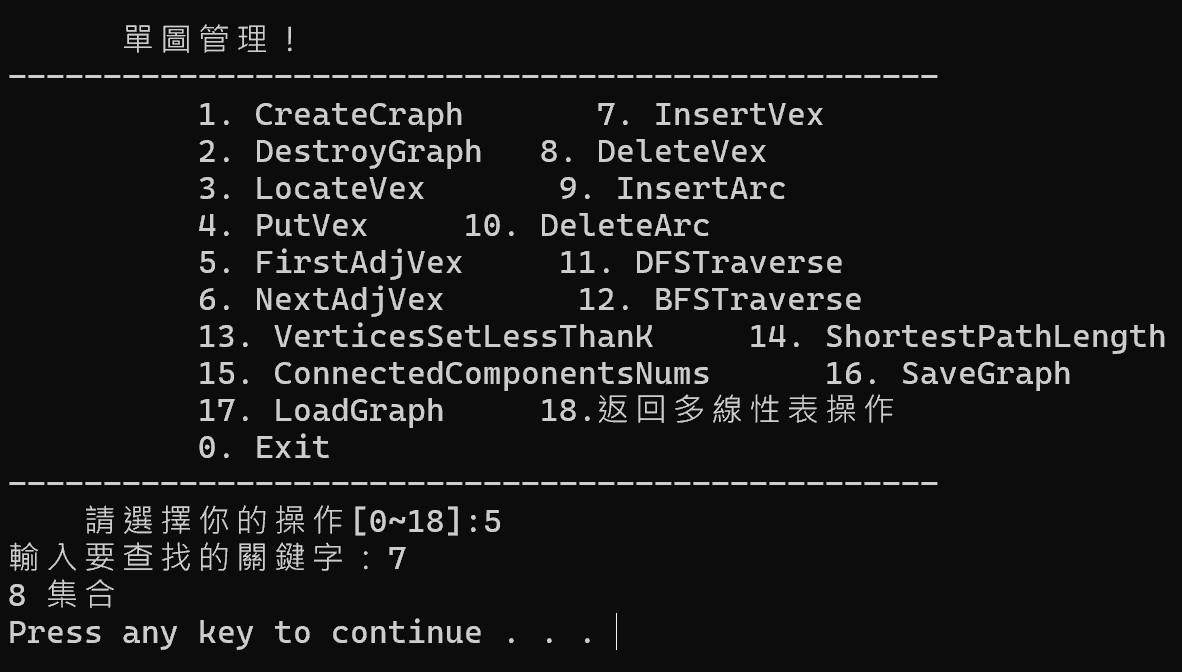
\includegraphics[scale=0.80]{images/2-7.jpg}
	\caption{获得第一邻接点}
	\label{fig2-7}
\end{center}
\end{figure}
\subsubsubsection{获得下一邻接点}
这里我们输入7 8看能否找到刚才顶点赋值9 有向图
\begin{figure}[H] % here top bottom
\begin{center}
	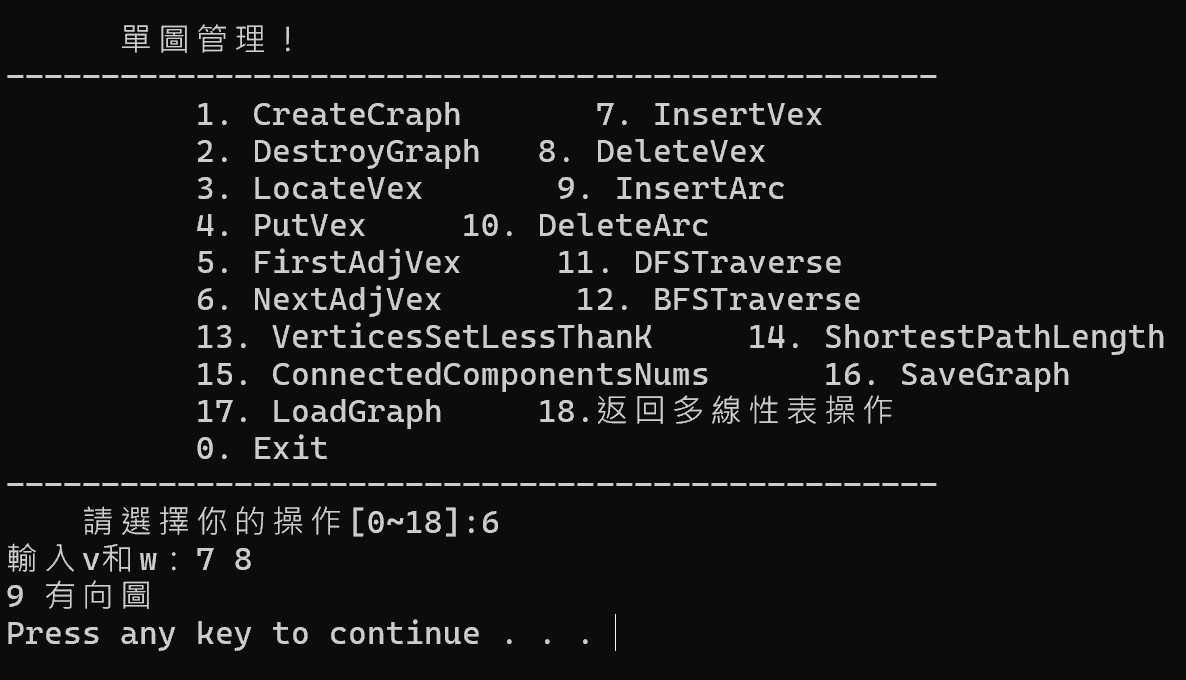
\includegraphics[scale=0.80]{images/2-8.jpg}
	\caption{获得下一邻接点}
	\label{fig2-8}
\end{center}
\end{figure}
\subsubsubsection{插入顶点}
这里输入6 无向图 插入顶点
\begin{figure}[H] % here top bottom
\begin{center}
	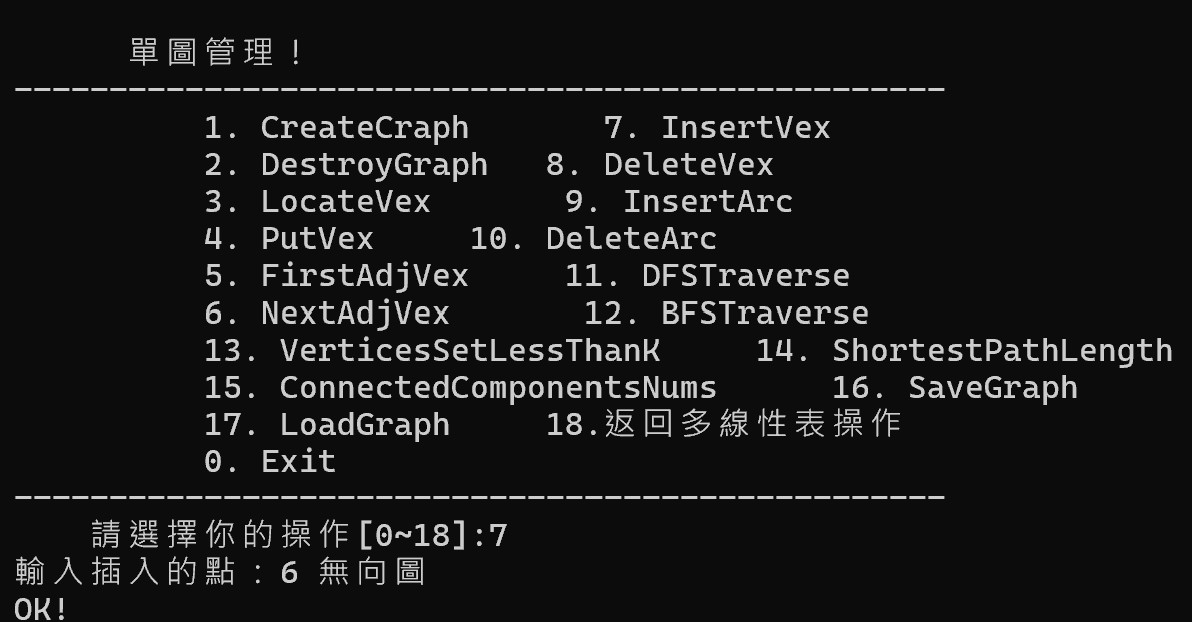
\includegraphics[scale=0.80]{images/2-9.jpg}
	\caption{插入顶点}
	\label{fig2-9}
\end{center}
\end{figure}
\subsubsubsection{删除顶点}
这里我们删除顶点9看能否成功删除
\begin{figure}[H] % here top bottom
\begin{center}
	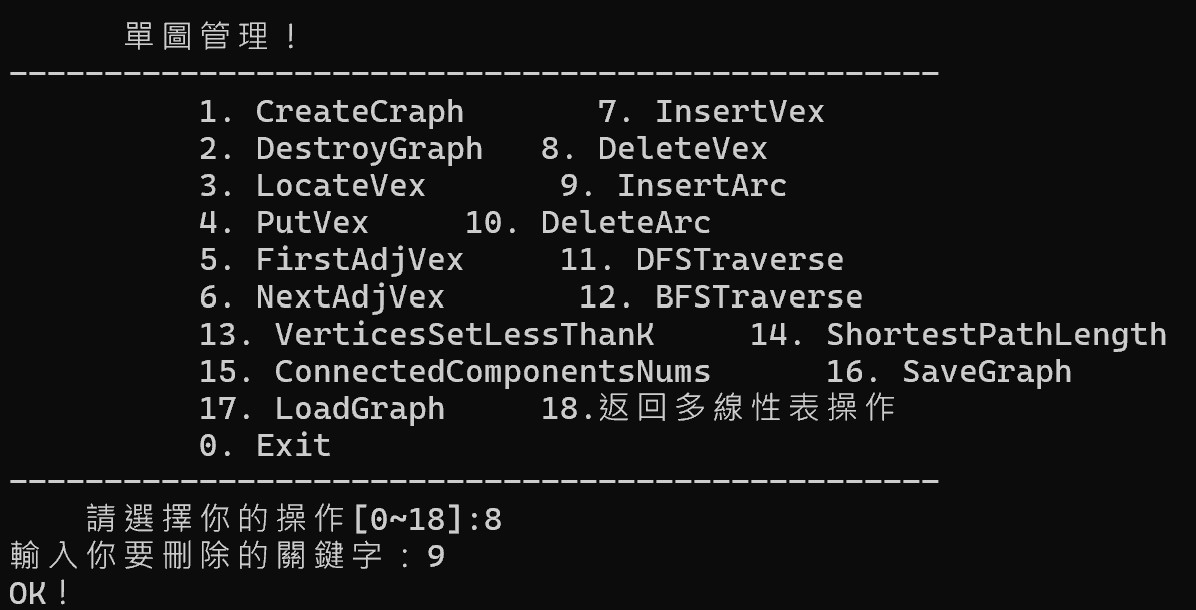
\includegraphics[scale=0.80]{images/2-10.jpg}
	\caption{删除顶点}
	\label{fig2-10}
\end{center}
\end{figure}
\subsubsubsection{深度优先搜索遍历}
我们遍历一下DFS看看结果，乱码只是输出字型问题不影响结果
\begin{figure}[H] % here top bottom
\begin{center}
	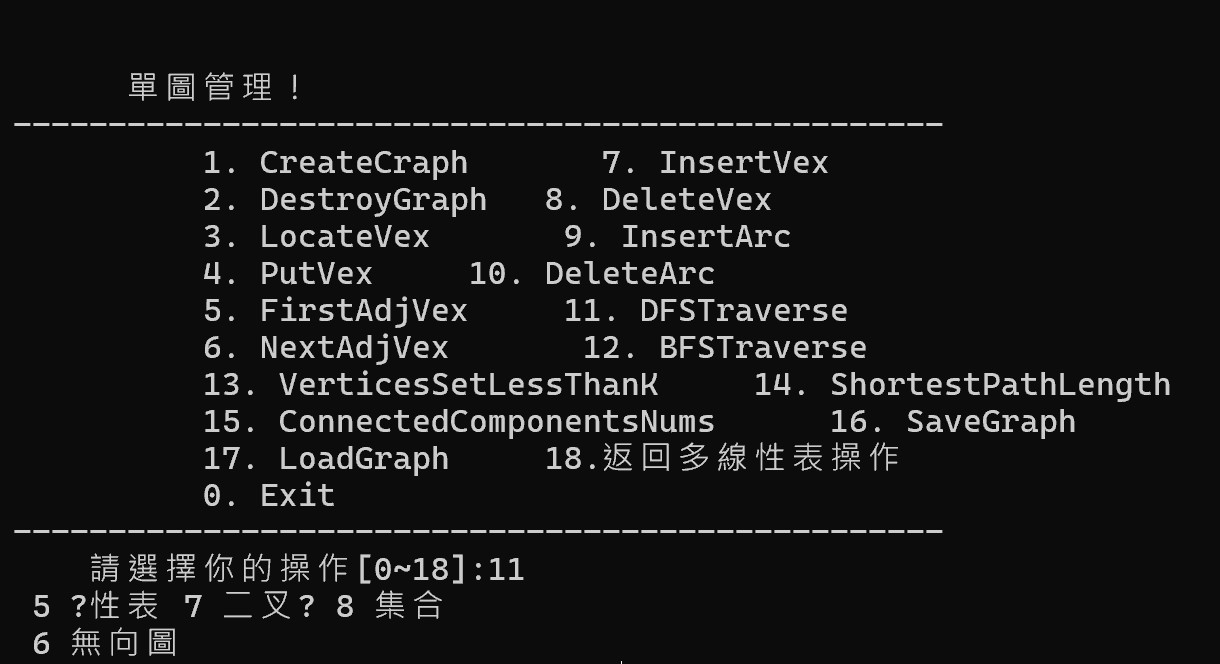
\includegraphics[scale=0.80]{images/2-11.jpg}
	\caption{深度优先搜索遍历}
	\label{fig2-11}
\end{center}
\end{figure}
\subsubsubsection{广度优先搜索遍历}
我们遍历一下BFS看看结果，乱码只是输出字型问题不影响结果
\begin{figure}[H] % here top bottom
\begin{center}
	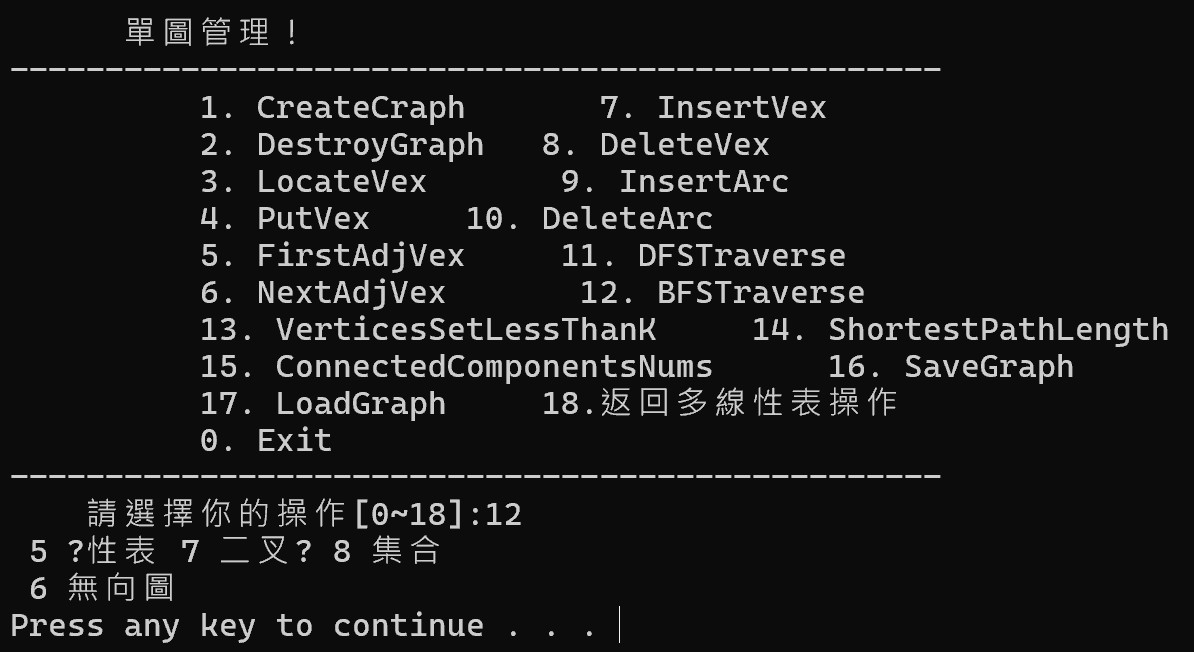
\includegraphics[scale=0.80]{images/2-12.jpg}
	\caption{广度优先搜索遍历}
	\label{fig2-12}
\end{center}
\end{figure}
\subsubsubsection{文件保存与读入}
这里我们存为graph，然后再读入一次graph。之后看下后面的操作是否能正常操作
\begin{figure}[H] % here top bottom
\begin{center}
	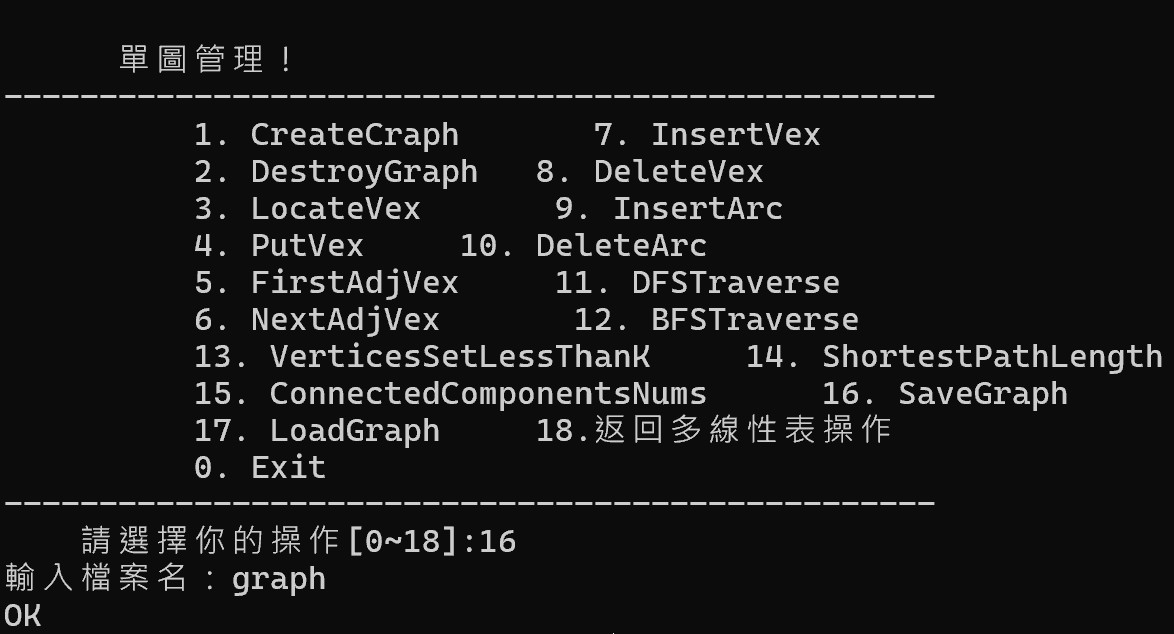
\includegraphics[scale=0.80]{images/2-13.jpg}
	\caption{文件保存}
	\label{fig2-13}
\end{center}
\end{figure}
\begin{figure}[H] % here top bottom
\begin{center}
	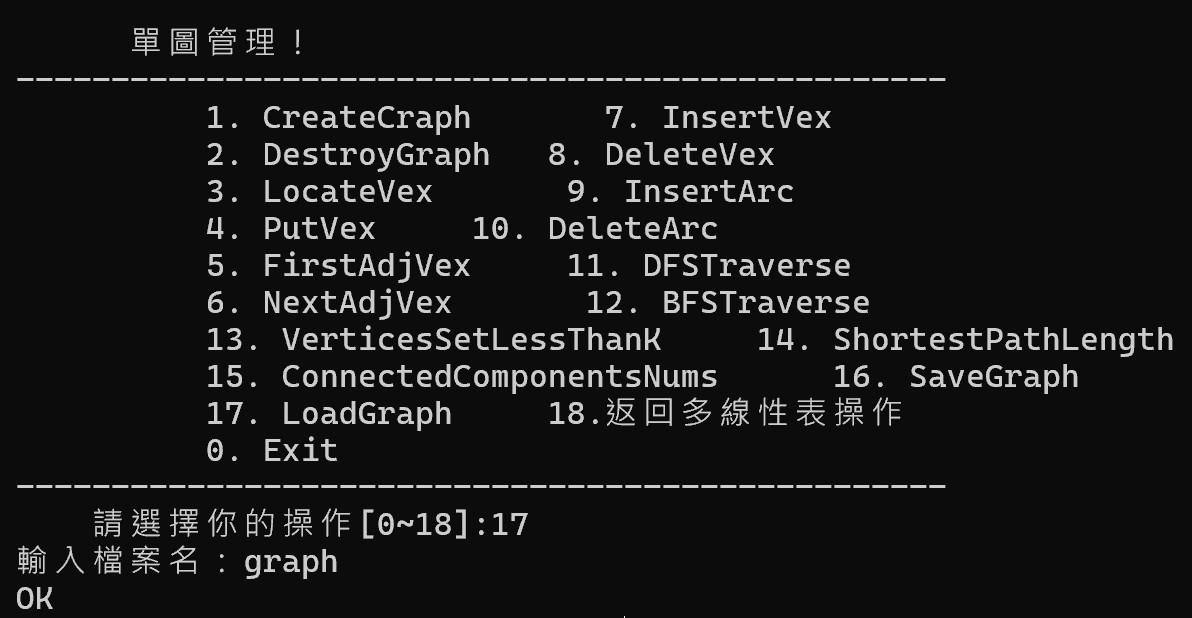
\includegraphics[scale=0.80]{images/2-14.jpg}
	\caption{文件读入}
	\label{fig2-14}
\end{center}
\end{figure}
\subsubsubsection{插入弧}
这里我们插入一下6 9看下是否能看看插入失败
\begin{figure}[H] % here top bottom
\begin{center}
	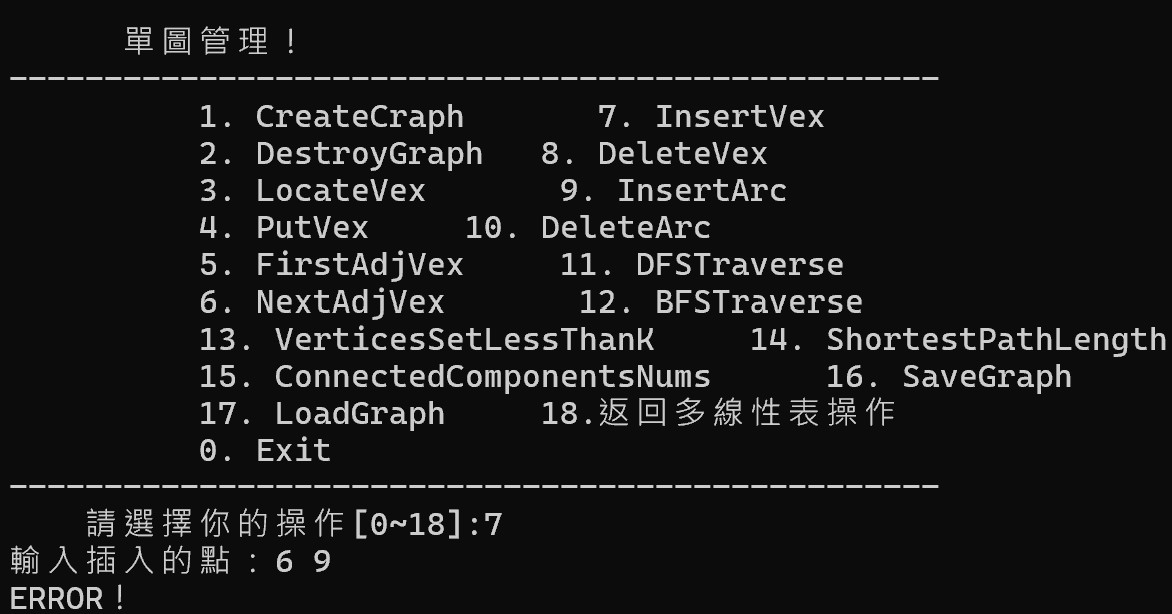
\includegraphics[scale=0.80]{images/2-15.jpg}
	\caption{插入弧}
	\label{fig2-15}
\end{center}
\end{figure}
\subsubsubsection{删除弧}
这里我们输入一下6 9看下是否能判断弧不存在
\begin{figure}[H] % here top bottom
\begin{center}
	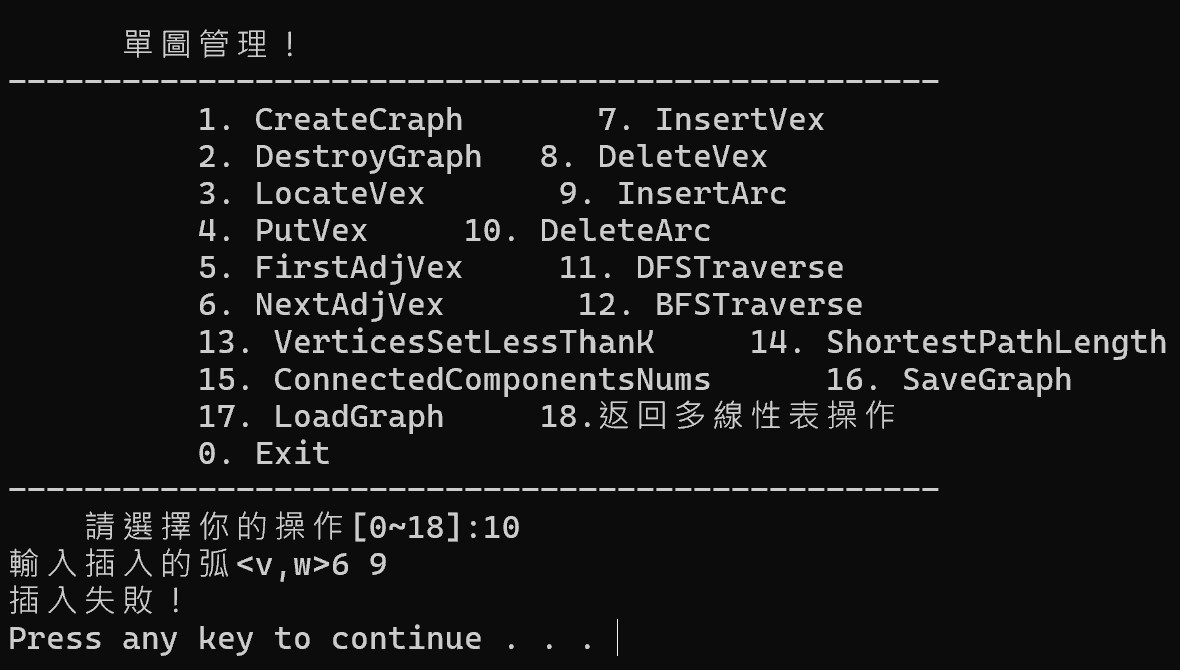
\includegraphics[scale=0.80]{images/2-16.jpg}
	\caption{删除弧}
	\label{fig2-16}
\end{center}
\end{figure}
\subsubsubsection{距离小于k的顶点集合}
我们输入5 8看看能否找到这些顶点集
\begin{figure}[H] % here top bottom
\begin{center}
	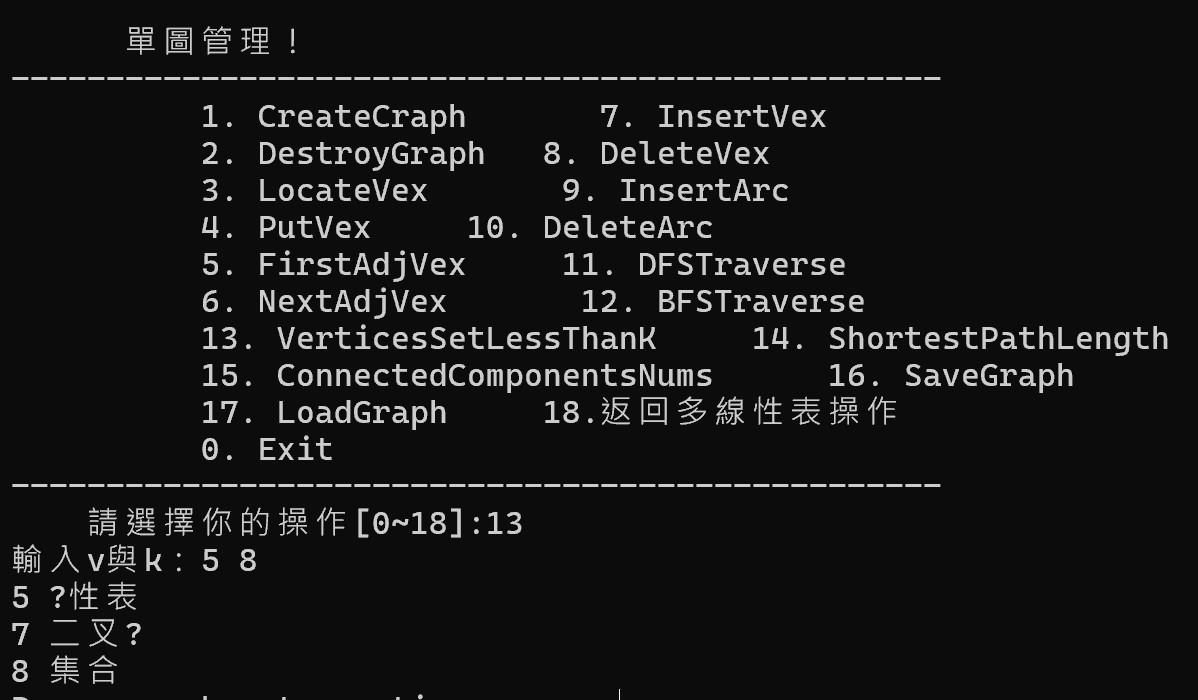
\includegraphics[scale=0.80]{images/2-17.jpg}
	\caption{距离小于k的顶点集合}
	\label{fig2-17}
\end{center}
\end{figure}
\subsubsubsection{顶点间最短路径和长度}
我们看看5 8的最短路径是不是2
\begin{figure}[H] % here top bottom
\begin{center}
	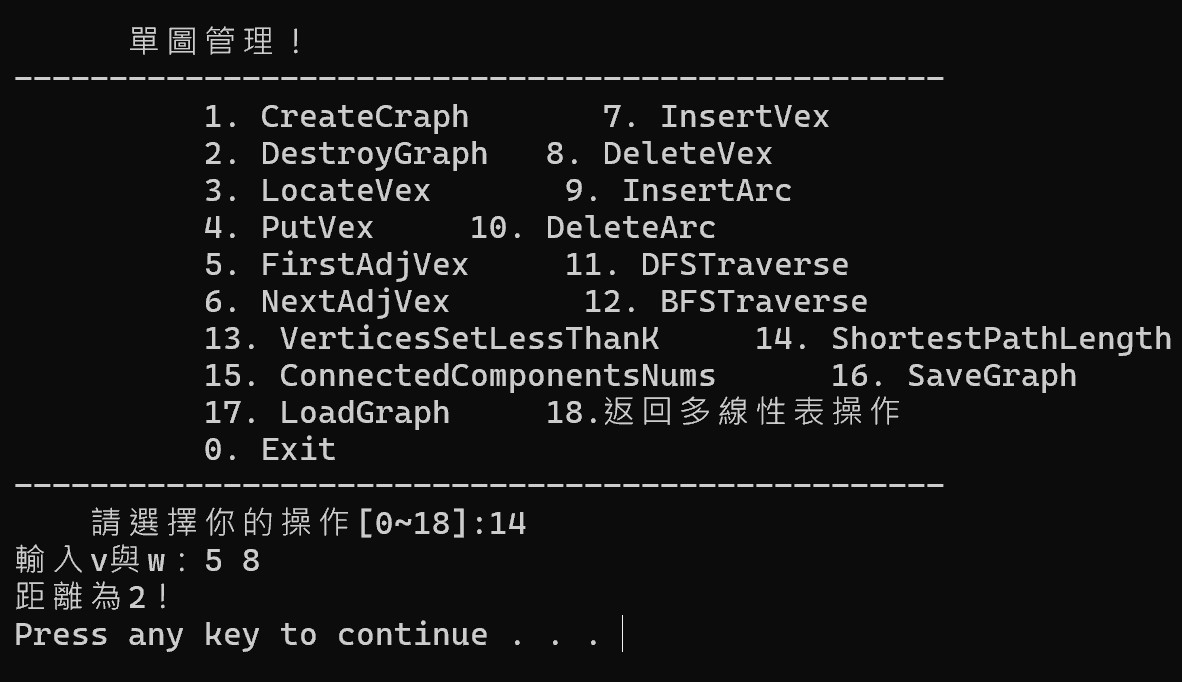
\includegraphics[scale=0.80]{images/2-18.jpg}
	\caption{顶点间最短路径和长度}
	\label{fig2-18}
\end{center}
\end{figure}
\subsubsubsection{图的连通分量}
我们查看下能否成功输出2
\begin{figure}[H] % here top bottom
\begin{center}
	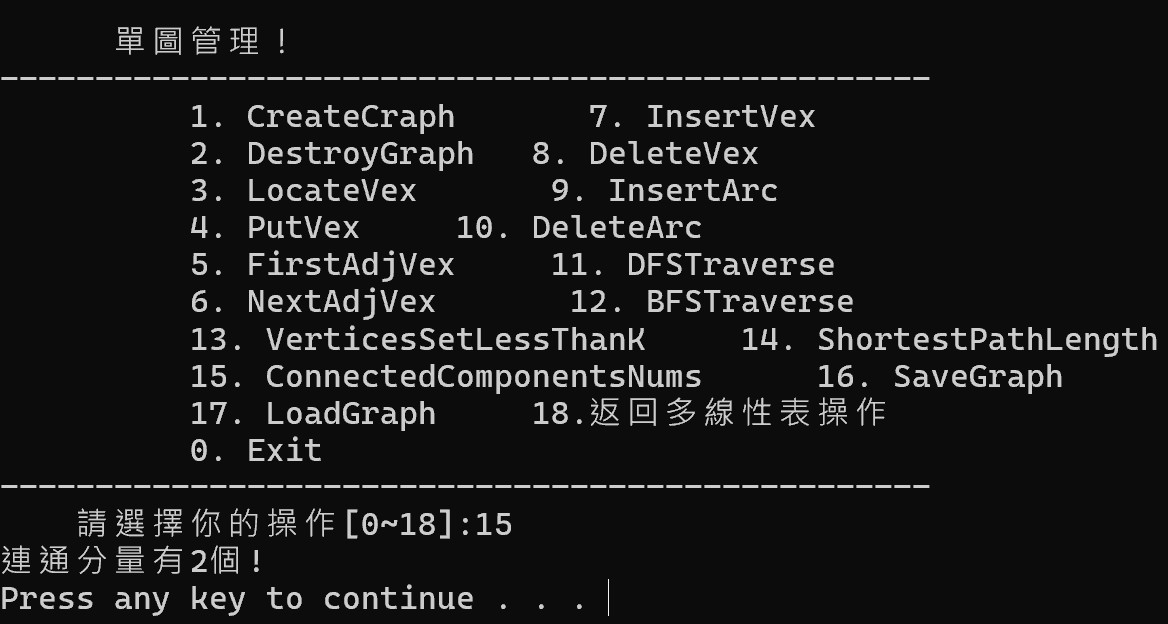
\includegraphics[scale=0.80]{images/2-19.jpg}
	\caption{图的连通分量}
	\label{fig2-19}
\end{center}
\end{figure}

\subsection{实验小结}
本次实验基于 C 语言实现了基于邻接表的图数据结构及其多图管理系统，核心目标是通过编程实践深入理解图的基本概念和操作。在基本实现方面，采用邻接表作为图的存储结构，通过AdjList数组存储顶点信息，每个顶点的邻接关系通过链表表示。通过这种结构，实现了图的基本操作，包括顶点的插入与删除、边的添加与删除、图的遍历（深度优先和广度优先）等。在多图管理上，设计了GRAPHS结构体，通过数组管理多个图实例，并实现了图的添加、切换和删除功能。
在实现过程中，我深刻体会到数据结构选择对程序性能的影响。邻接表在存储稀疏图时的优势明显，相较于邻接矩阵可以节省大量存储空间。同时，通过实践掌握了链表操作在图结构中的应用，包括节点的动态分配与释放、链表的遍历与修改等。在处理图的遍历操作时，理解了递归与队列在深度优先和广度优先算法中的不同应用场景。

\newpage

\nocite{*} %% 作用是不对文献进行引用，但可以生成文献列表

\bibliographystyle{Experimental_Report}
\bibliography{Experimental_Report}
\setcounter{secnumdepth}{0}
\appendix

\section{附录A 基于顺序存储结构线性表实现的源程序}

\begin{lstlisting}[style=commonCodeStyle, caption={目标程序}, label={lst:2-17}]
/* Linear Table On Sequence Structure */
#include <stdio.h>
#include <malloc.h>
#include <stdlib.h>
#include <string.h>
#include <algorithm>

/*---------page 10 on textbook ---------*/
#define TRUE 1
#define FALSE 0
#define OK 1
#define ERROR 0
#define INFEASIBLE -1
#define OVERFLOW -2

typedef int status; 
typedef int ElemType;

/*-------page 22 on textbook -------*/
#define LIST_INIT_SIZE 100
#define LISTINCREMENT  10

typedef struct{
	ElemType * elem;
	int length;
	int listsize;
}SqList;

typedef struct{
	struct { 
		char name[30];
		SqList L;    
	} elem[10];
	int length;
}LISTS;

LISTS Lists; 
ElemType count = 0;
SqList L;

/*-----page 19 on textbook ---------*/
status InitList(SqList& L);
status DestroyList(SqList& L);
status ClearList(SqList& L);
status ListEmpty(SqList L);
int ListLength(SqList L);
status GetElem(SqList L, int i, ElemType& e);
status LocateElem(SqList L, ElemType e); 
status PriorElem(SqList L, ElemType cur, ElemType &pre_e);
status NextElem(SqList L, ElemType cur, ElemType& next_e);
status ListInsert(SqList &L, int i, ElemType e);
status ListDelete(SqList &L, int i, ElemType& e);
status ListTraverse(SqList L);  

int maxSubArraySum(SqList L) {
	int max = L.elem[0];
	for (int i = 0; i < L.length; i++) {
		int sum = 0; 
		for (int j = i; j < L.length; j++) {
			sum += L.elem[j]; 
			if (sum > max) {
				max = sum; 
			}
		}
	}
	return max;
}

int SubArrayNum(SqList L, int k) {
	int count = 0;
	for (int i = 0; i < L.length; i++) {
		int sum = 0;
		for (int j = i; j < L.length; j++) {
			sum += L.elem[j]; 
			if (sum == k) {
				count++; 
			}
		}
	}
	return count;
}

void sortList(SqList& L) {
	std::sort(L.elem, L.elem + L.length);
}

status  SaveList(SqList L, char FileName[])
{
	if(L.elem == NULL) return INFEASIBLE;
	FILE *w = fopen(FileName, "w");
	if (w == NULL) return INFEASIBLE;
	for(int i = 0; i < L.length; i++){
		fprintf(w, "%d ", L.elem[i]);
	}
	fclose(w);
	return OK;
}

status LoadList(SqList &L, char FileName[])
{
	int t;
	if (L.elem != NULL) {
		DestroyList(L);
	}
	InitList(L);
	FILE *r = fopen(FileName, "r");
	if (r == NULL) return INFEASIBLE;
	while(fscanf(r, "%d", &t) != EOF){
	ListInsert(L, L.length + 1, t);
}
fclose(r);
return OK;
}

status AddList(LISTS &Lists, char ListName[])
{
InitList(Lists.elem[Lists.length].L);
strcpy(Lists.elem[Lists.length].name, ListName);
Lists.length++;
return OK;
}

status RemoveList(LISTS &Lists, char ListName[])
{
for(int i = 0; i < Lists.length; i++)
{
	if(strcmp(ListName, Lists.elem[i].name) == 0)
	{
		DestroyList(Lists.elem[i].L);
		for(int j = i; j < Lists.length - 1; j++)
		{
			Lists.elem[j] = Lists.elem[j + 1];
		}
		Lists.length--;
		return OK;
	}
}
return ERROR;
}

int LocateList(LISTS Lists, char ListName[])
{
for(int i = 0; i < Lists.length; i++)
{
	if(strcmp(ListName, Lists.elem[i].name) == 0)
	{
		count = i + 1;
		// 复制 elem[i].L 到 L
		if (L.elem != NULL) {
			DestroyList(L);
		}
		InitList(L);
		for (int j = 0; j < Lists.elem[i].L.length; j++) {
			ElemType e;
			GetElem(Lists.elem[i].L, j + 1, e);
			ListInsert(L, j + 1, e);
		}
		return i + 1;
	}
}
return 0;
}

// 复制 L 到 elem[i]
void copyListToElem(LISTS &Lists, int index, SqList L) {
if (Lists.elem[index].L.elem != NULL) {
	DestroyList(Lists.elem[index].L);
}
InitList(Lists.elem[index].L);
for (int i = 0; i < L.length; i++) {
	ElemType e;
	GetElem(L, i + 1, e);
	ListInsert(Lists.elem[index].L, i + 1, e);
}
}

int k = 0;
char s1[100];

/*--------------------------------------------*/
int main(){
int op = 1, op1 = 1, op0 = 4, result, tp, e;
char name[100];

op0:
while(op0)
{
	system("cls");
	printf("\n\n");
	printf("\t      Menu for Linear Table On Sequence Structure \n");
	printf("\t-------------------------------------------------\n");
	printf("\t    	  1. 多表管理       \t2. 對當前表操作\n");
	printf("\t    	  0.結束\n       ");
	printf("\t-------------------------------------------------\n");
	
	printf("    請選擇你的操作[0~2]:");
	scanf("%d", &op0);
	switch(op0)
	{
		case 1:
		{
			op1 = 100;
			goto op1;
			break;
		}
		case 2:
		{
			op = 100;
			goto op;
			break;
		}
		case 0:
		{
			printf("GG");
			return 0;
			break;
		}
		default:
		{
			printf("無效輸入請重新輸入\n");
		}
	}
	system("PAUSE");
}
op1:
while(op1)
{
	system("cls");
	printf("\n\n");
	printf("\t      Menu for Linear Table On Sequence Structure \n");
	printf("\t-------------------------------------------------\n");
	printf("\t    	  1. 創立表      \t3. 刪除表\n");
	printf("\t    	  2. 查找表      \t0. 返回\n");
	printf("\t------------------------------------------------\n");
	
	printf("    請選擇你的操作[0~3]:\n");
	scanf("%d", &op1);
	switch(op1)
	{
		case 1:
		{
			printf("Name for the new list\n");
			scanf("%s", name);
			AddList(Lists, name);
			printf("success\n"); 
			break;
		}
		case 2:
		{
			printf("Name for the list\n");
			scanf("%s", name);
			result = LocateList(Lists, name);
			if (result != 0) printf("success\n");
			if (result == 0) printf("查無此表\n");
			break;
		}
		case 3:
		{
			printf("Delete the List:(input list's name)\n");
			scanf("%s", name);
			result = RemoveList(Lists, name);
			if (result == OK)
			{
				printf("OK\n");
				
			}
			else
			{
				printf("刪除失敗\n");
			}//if (result == (INFEASIBLE || ERROR)) printf("刪除失敗\n");
			
			break;
		}
		case 0:
		{
			op0 = 4;
			goto op0;
			break;
		}
		default:
		{
			printf("輸入有誤，請重新輸入\n");
			break;
		}
	}
	system("PAUSE");
}
op:
while(op){
	system("cls");
	printf("\n\n");
	printf("\t      Menu for Linear Table On Sequence Structure \n");
	printf("\t-------------------------------------------------\n");
	printf("\t    	  1. InitList       \t7. LocateElem\n");
	printf("\t    	  2. DestroyList    \t8. PriorElem\n");
	printf("\t    	  3. ClearList       \t9. NextElem \n");
	printf("\t    	  4. ListEmpty     \t10. ListInsert\n");
	printf("\t    	  5. ListLength     \t11. ListDelete\n");
	printf("\t    	  6. GetElem       \t12. ListTrabverse\n\n");
	printf("\t    	  13. MaxSubArray  \t14. SubArrayNum\n");
	printf("\t    	  15. sortList      \t16. Savelist\n");
	printf("\t    	  17. LoadFile  \t18. WithMultiLists\n");
	printf("\t          0. turn back\n");
	printf("\t-------------------------------------------------\n");
	printf("    請選擇你的操作[0~18]:");
	scanf("%d", &op);
	switch(op){
		case 1:
		result = InitList(L);
		if (result == OK) printf("OK\n");
		if (result == INFEASIBLE) printf("線性表已存在！\n");               
		break;
		case 2:
		result = DestroyList(L);
		if (result == OK) printf("OK\n");
		if (result == INFEASIBLE) printf("線性表不存在！\n");
		break;
		case 3:
		result = ClearList(L);
		if (result == OK) printf("OK\n");
		if (result == INFEASIBLE) printf("線性表不存在！\n");               
		break;
		case 4:
		result = ListEmpty(L);
		if (result == TRUE) printf("線性表為空！\n");
		if(result == FALSE) printf("線性表不為空！\n");
		if (result == INFEASIBLE) printf("線性表不存在！\n");               
		break;
		case 5:
		result = ListLength(L);
		if (result == INFEASIBLE) printf("線性表不存在！\n");   
		else printf("線性表長度為%d\n", result);
		break;
		case 6:
		printf("獲取線性表的第i個元素：");
		scanf("%d", &tp);
		result = GetElem(L, tp, e);
		if (result == ERROR) printf("查找失敗！\n");
		if (result == INFEASIBLE) printf("線性表不存在！\n");
		if(result == OK) printf("第%d個元素為%d\n", tp, e);   
		break;
		case 7:
		printf("輸入你要查找的元素：");
		scanf("%d", &tp);
		result = LocateElem(L, tp);       
		if (result == ERROR) printf("查找失敗！\n");
		else if (result == INFEASIBLE) printf("線性表不存在！\n");
		else printf("第%d個元素為%d\n", result, tp);                   
		break;
		case 8:
		printf("輸入你要查找的元素前驅：");
		scanf("%d", &tp);
		result = PriorElem(L, tp, e);       
		if (result == ERROR) printf("查找失敗！\n");
		else if (result == INFEASIBLE) printf("線性表不存在！\n");
		else printf("%d的前驅為%d\n", tp, e);
		break;
		case 9:
		printf("輸入你要查找的元素後繼：");
		scanf("%d", &tp);
		result = NextElem(L, tp, e);       
		if (result == ERROR) printf("查找失敗！\n");
		else if (result == INFEASIBLE) printf("線性表不存在！\n");
		else printf("%d的後繼為%d\n", tp, e);
		break;
		case 10:
		printf("輸入在第i個元素前插入的元素：");
		scanf("%d%d", &tp, &e);
		result = ListInsert(L, tp, e);
		if (result == ERROR) printf("插入失敗！\n");
		else if (result == INFEASIBLE) printf("線性表不存在！\n");
		else printf("OK\n");                
		break;
		case 11:
		printf("輸入你要刪除的第i個元素：");
		scanf("%d", &tp);
		result = ListDelete(L, tp, e);       
		if (result == ERROR) printf("查找失敗！\n");
		else if (result == INFEASIBLE) printf("線性表不存在！\n");
		else printf("已刪除第%d個元素%d\n", tp, e);
		break;
		case 12:
		result = ListTraverse(L);
		if (result == INFEASIBLE) printf("線性表不存在！\n");
		break;
		case 13:
		result = maxSubArraySum(L);
		printf("最大子數組和是%d", result);
		if (result == INFEASIBLE) printf("線性表不存在！\n");
		break;
		case 14:
		printf("設定子數組和");
		scanf("%d", &k);
		result = SubArrayNum(L, k);
		printf("有%d個", result);
		if (result == INFEASIBLE) printf("線性表不存在！\n");
		break;
		case 15:
		sortList(L);
		printf("己sort,let try");
		if (result == INFEASIBLE) printf("線性表不存在！\n");
		break;
		case 16:
		printf("輸入保存文件名");
		scanf("%s", s1);
		result = SaveList(L, s1);
		if (result == INFEASIBLE) printf("線性表不存在！\n");
		break;
		case 17:
		printf("輸入加載文件名");
		scanf("%s", s1);   
		result = LoadList(L, s1);
		if (result == INFEASIBLE) printf("線性表不存在！\n");
		break;
		case 18:
		result = ListTraverse(L);
		if (result == INFEASIBLE) printf("線性表不存在！\n");
		break;
		case 0:
		// 操作完把 L 复制回 elem[i]
		if (count > 0) {
			copyListToElem(Lists, count - 1, L);
		}
		// 重置 L
		if (L.elem != NULL) {
			DestroyList(L);
		}
		InitList(L);
		op0 = 4;
		goto op0;
		break;
	}//end of switch
	system("PAUSE");
}//end of while
return 0;
}//end of main()

status InitList(SqList& L)
{
if(L.elem == NULL)
{
	L.elem = (ElemType *) malloc(sizeof(ElemType) * LIST_INIT_SIZE);
	L.length = 0;
	L.listsize = LIST_INIT_SIZE;
	return OK;
}
else
{
	return INFEASIBLE;
}
}

status DestroyList(SqList& L)
{
if(L.elem != NULL)
{
	free(L.elem);
	L.elem = NULL;
	L.length = 0;
	L.listsize = 0;
	return OK;
}
else
{
	return INFEASIBLE;
}
}

status ClearList(SqList& L)
{
if(L.elem != NULL)
{
	L.length = 0;
	return OK;
}
else
{
	return INFEASIBLE;
}
}

status ListEmpty(SqList L)
{
if(L.elem == NULL)
{
	return INFEASIBLE;
}
if(L.length == 0)
{
	return TRUE;
}
else
{
	return FALSE;
}
}

status ListLength(SqList L)
{
if(L.elem != NULL)
{
	return L.length;
}
else
{
	return INFEASIBLE;
}
}

status GetElem(SqList L, int i, ElemType &e)
{
if(i < 1 || i > L.length)
{
	return ERROR;
}
if(L.elem != NULL)
{
	e = L.elem[i - 1];
	return OK;
}
else
{
	return INFEASIBLE;
}
}

int LocateElem(SqList L, ElemType e)
{
if(L.elem != NULL)
{
	for(int i = 0; i < L.length; i++)
	{
		if(e == L.elem[i])
		{
			return i + 1;
		}
	}
	return 0;
}
else
{
	return INFEASIBLE;
}
}

status PriorElem(SqList L, ElemType e, ElemType &pre)
{
if(L.elem != NULL)
{
	for(int i = 1; i < L.length; i++)
	{
		if(e == L.elem[i])
		{
			pre = L.elem[i - 1];
			return OK;
		}
	}
	return ERROR;
}
else
{
	return INFEASIBLE;
}
}

status NextElem(SqList L, ElemType e, ElemType &next)
{
if(L.elem != NULL)
{
	for(int i = 1; i < L.length - 1; i++)
	{
		if(e == L.elem[i])
		{
			next = L.elem[i + 1];
			return OK;
		}
	}
	return ERROR;
}
else
{
	return INFEASIBLE;
}
}

status ListInsert(SqList &L, int i, ElemType e)
{
if(L.elem == NULL) return INFEASIBLE;
if(i < 1 || i > L.length + 1) return ERROR;  
if(L.length >= L.listsize){
	int *newbase = (int *)realloc(L.elem, (L.listsize + LISTINCREMENT) * sizeof(int));
	if(newbase == NULL) return 0;
	L.listsize += LISTINCREMENT;
	L.elem = newbase;
}
for(int j = L.length; j > i - 1; j--){
	L.elem[j] = L.elem[j - 1];
}
L.elem[i - 1] = e;
L.length++;
return OK;
}

status ListDelete(SqList &L, int i, ElemType &e)
{
if(L.elem == NULL)
{
	return INFEASIBLE;
}
if(i <= 0 || i > L.length)
{
	return ERROR;
}
e = L.elem[i - 1];
for(int j = i - 1; j < L.length - 1; j++)
{
	L.elem[j] = L.elem[j + 1];
}
L.length--;
return OK;
}

status ListTraverse(SqList L)
{
if(L.elem == NULL)
{
	return INFEASIBLE;
}
for(int i = 0; i < L.length; i++)
{
	printf("%d", L.elem[i]);
	if(i < L.length - 1)
	{
		printf(" ");
	}
}
printf("\n");
return OK;
}    	
\end{lstlisting}
\newpage
\section{附录B 基于链式存储结构线性表实现的源程序}
\begin{lstlisting}[style=commonCodeStyle, caption={目标程序}, label={lst:2-17}]
/* Linear Table On Sequence Structure */
#include <stdio.h>
#include <iostream>
#include <algorithm>
#include <malloc.h>
#include <stdlib.h>
#include <string.h>
/*---------page 10 on textbook ---------*/
#define TRUE 1
#define FALSE 0
#define OK 1
#define ERROR 0
#define INFEASIBLE -1 
#define OVERFLOW -2

typedef int status; 
typedef int ElemType; //資料元素類型定義

/*-------page 22 on textbook -------*/
#define LIST_INIT_SIZE 100
#define LISTINCREMENT  10
typedef struct LNode{  //單鏈表（鏈式結構）結點的定義
	ElemType data;
	struct LNode *next;
}LNode,*LinkList;
LinkList L,Ltemp;
typedef struct{  //線性表的集合類型定義
	struct { char name[30];
		LinkList L;    
	} elem[10];
	int length;
}LISTS;
LISTS Lists;      //線性表集合的定義Lists
/*-----page 19 on textbook ---------*/
status InitList(LinkList &L);
status DestroyList(LinkList &L);
status ClearList(LinkList &L);
status ListEmpty(LinkList L);
int ListLength(LinkList L);
status GetElem(LinkList L,int i,ElemType &e);
status LocateElem(LinkList L,ElemType e);
status PriorElem(LinkList L,ElemType e,ElemType &pre);
status NextElem(LinkList L,ElemType e,ElemType &next);
status ListInsert(LinkList &L,int i,ElemType e);
status ListDelete(LinkList &L,int i,ElemType &e);
status ListTraverse(LinkList L);
status SaveList(LinkList L,char FileName[]);
status LoadList(LinkList &L,char FileName[]);
status AddList(LISTS &Lists,char ListName[]);
status RemoveList(LISTS &Lists,char ListName[]);
int LocateList(LISTS Lists,char ListName[]);
status reverseList(LinkList L);
int RemoveNthFromEnd(LinkList L,int k);
int sortList(LinkList L);
//簡化過
/*--------------------------------------------*/
int main(){
	int op=1,result,tp,e,k,op1=1,t;
	char ch[1000];
	char name[30];
	while(op1){
	system("cls");  printf("\n\n");
	printf("-------------------------------------------------\n");
	printf("1.進入多線性表管理        2.進入單線性表管理\n");
	printf("0. Exit\n");
	printf("-------------------------------------------------\n");
	scanf("%d",&op1);   
	switch(op1){
	case 1:
	op=1;
	while(op!=0 and op!=4){
	t=0;
	system("cls");  printf("\n\n");
	printf("      多線性表管理！     \n");         
	printf("-------------------------------------------------\n");
	printf("          1. AddList       3. LocateList\n");
	printf("          2. DestroyList   4. 返回選擇頁面\n");       
	printf("          0.Exit\n");   
	printf("-------------------------------------------------\n");
	printf("    請選擇你的操作[0~4]:");        
	scanf("%d",&op);
	switch(op){
	case 1:
		printf("添加一個線性表，請輸入線性表名稱：");	
		scanf("%s",name);
		result=AddList(Lists,name);                 
		if(result==OK) printf("OK!\n");
		break;
	case 2:
	printf("刪除一個線性表，請輸入線性表名稱：");
	scanf("%s",name);
	result=RemoveList(Lists,name);                  
	if(result==OK) printf("OK!\n");
	else printf("線性表不存在！\n");               
	break;
	case 3:
	printf("查找一個線性表，請輸入線性表名稱：");
	scanf("%s",name);
	result=LocateList(Lists,name);                  
	if(result==ERROR) printf("線性表不存在！\n");
	else{
		int t;
		printf("OK!  按1對其進行單線性表操作,按其他按鈕返回");
		scanf("%d",&t);
		if(t==1){
			L=Lists.elem[result-1].L;
			while(op!=0 and op!=18){
				int t=0;
				system("cls");  printf("\n\n");
				printf("      單線性表管理！     \n");
				printf("-------------------------------------------------\n");
				printf("          1. InitList       7. LocateElem\n");
				printf("          2. DestroyList   8. PriorElem\n");
				printf("          3. ClearList       9. NextElem \n");
				printf("          4. ListEmpty     10. ListInsert\n");
				printf("          5. ListLength     11. ListDelete\n");
				printf("          6. GetElem       12. ListTrabverse\n");
				printf("          13. reverseList     14. RemoveNthFromEnd\n");
				printf("          15. sortList       16. SaveList\n");
				printf("          17. LoadList      18.返回多線性表操作\n");    
				printf("          0. Exit\n");
				printf("-------------------------------------------------\n");
				printf("    請選擇你的操作[0~18]:");
				scanf("%d",&op);
				switch(op){
					case 1:
					result=InitList(L);
					if (result==OK) printf("OK\n");
					if (result==INFEASIBLE) printf("線性表已存在！\n");               
					break;
					case 2:
					result=DestroyList(L);
					if (result==OK) printf("OK\n");
					if (result==INFEASIBLE) printf("線性表不存在！\n");
					break;
					case 3:
					result=ClearList(L);
					if (result==OK) printf("OK\n");
					if (result==INFEASIBLE) printf("線性表不存在！\n");                
					break;
					case 4:
					result=ListEmpty(L);
					if (result==TRUE) printf("線性表為空！\n");
					if(result==FALSE) printf("線性表不為空！\n");
					if (result==INFEASIBLE) printf("線性表不存在！\n");                    
					break;
					case 5:
					result= ListLength(L);
					if (result==INFEASIBLE) printf("線性表不存在！\n");    
					else printf("線性表長度為%d\n",result);
					break;
					case 6:
					printf("獲取線性表的第i個元素：");
					scanf("%d",&tp);
					result=GetElem(L,tp,e);
					if (result==ERROR) printf("查找失敗！\n");
					if (result==INFEASIBLE) printf("線性表不存在！\n");
					if(result==OK) printf("第%d個元素為%d\n",tp,e);  
					break;
					case 7:
					printf("輸入你要查找的元素：");
					scanf("%d",&tp);
					result=LocateElem(L,tp);         
					if (result==ERROR) printf("查找失敗！\n");
					else if (result==INFEASIBLE) printf("線性表不存在！\n");
					else printf("第%d個元素為%d\n",result,tp);                   
					break;
					case 8:
					printf("輸入你要查找的元素前驅：");
					scanf("%d",&tp);
					result=PriorElem(L,tp,e);        
					if (result==ERROR) printf("查找失敗！\n");
					else if (result==INFEASIBLE) printf("線性表不存在！\n");
					else printf("%d的前驅為%d\n",tp,e);
					break;
					case 9:
					printf("輸入你要查找的元素後繼：");
					scanf("%d",&tp);
					result=NextElem(L,tp,e);         
					if (result==ERROR) printf("查找失敗！\n");
					else if (result==INFEASIBLE) printf("線性表不存在！\n");
					else printf("%d的後繼為%d\n",tp,e);
					break;
					case 10:
					printf("輸入在第i個元素前插入的元素：");
					scanf("%d%d",&tp,&e);
					result=ListInsert(L,tp,e);
					if (result==ERROR) printf("插入失敗！\n");
					else if (result==INFEASIBLE) printf("線性表不存在！\n");
					else printf("OK\n");                
					break;
					case 11:
					printf("輸入你要刪除的第i個元素：");
					scanf("%d",&tp);
					result=ListDelete(L,tp,e);       
					if (result==ERROR) printf("查找失敗！\n");
					else if (result==INFEASIBLE) printf("線性表不存在！\n");
					else printf("已刪除第%d個元素%d\n",tp,e);
					break;
					case 12:
					result= ListTraverse(L);
					if (result==INFEASIBLE) printf("線性表不存在！\n");
					break;
					case 13:
					result=reverseList(L);
					if (result==INFEASIBLE) printf("線性表不存在！\n");
					else printf("OK!\n");   
					break;       
					case 14:
					printf("刪除倒數第n個數:");
					scanf("%d",&k);
					result=RemoveNthFromEnd(L,k);
					if (result==INFEASIBLE) printf("線性表不存在或為空！\n");
					else if(result == ERROR) printf("刪除失敗！\n");
					else printf("已刪除倒數第%d個數%d！\n",k,result);    
					break;      
					case 15:
					result=sortList(L);
					if (result==INFEASIBLE) printf("線性表不存在！\n");
					else printf("OK!\n");               
					break;  
					case 16:
					printf("輸入檔案名：");
					scanf("%s",ch);
					result=SaveList(L,ch);
					if (result==INFEASIBLE) printf("線性表不存在！\n");
					else printf("OK\n");                 
					break;
					case 17:
					printf("輸入檔案名：");
					scanf("%s",ch);
					result=LoadList(L,ch);
					if (result==INFEASIBLE) printf("線性表已存在！\n");
					else printf("OK\n");                        
					break;
					case 18:
					break;
					case 0:
					t=1;
					break;
					Lists.elem[result-1].L=L;   
				}//end of switch
				system("PAUSE");                
			}                               
		}
	}                                   
					break;
					case 4:
					break;
					case 0:
					t=1;
					break;                                                                      
				}       
				system("PAUSE");                        
				}
				break;
				
				case 2:
				op=1;
				L=Ltemp;
				while(op!=0 and op!=18){                
				t=0;
				system("cls");  printf("\n\n");
				printf("      單線性表管理！     \n");
				printf("-------------------------------------------------\n");
				printf("          1. InitList       7. LocateElem\n");
				printf("          2. DestroyList   8. PriorElem\n");
				printf("          3. ClearList       9. NextElem \n");
				printf("          4. ListEmpty     10. ListInsert\n");
				printf("          5. ListLength     11. ListDelete\n");
				printf("          6. GetElem       12. ListTrabverse\n");
				printf("          13. reverseList     14. RemoveNthFromEnd\n");
				printf("          15. sortList       16. SaveList\n");
				printf("          17. LoadList      18.返回選擇頁面\n");  
				printf("          0. Exit\n");
				printf("-------------------------------------------------\n");
				printf("    請選擇你的操作[0~18]:");
				scanf("%d",&op);
				switch(op){
				case 1:
				result=InitList(L);
				if (result==OK) printf("OK\n");
				if (result==INFEASIBLE) printf("線性表已存在！\n");               
				break;
				case 2:
				result=DestroyList(L);
				if (result==OK) printf("OK\n");
				if (result==INFEASIBLE) printf("線性表不存在！\n");
				break;
				case 3:
				result=ClearList(L);
				if (result==OK) printf("OK\n");
				if (result==INFEASIBLE) printf("線性表不存在！\n");                
				break;
				case 4:
				result=ListEmpty(L);
				if (result==TRUE) printf("線性表為空！\n");
				if(result==FALSE) printf("線性表不為空！\n");
				if (result==INFEASIBLE) printf("線性表不存在！\n");                    
				break;
				case 5:
				result= ListLength(L);
				if (result==INFEASIBLE) printf("線性表不存在！\n");    
				else printf("線性表長度為%d\n",result);
				break;
				case 6:
				printf("獲取線性表的第i個元素：");
				scanf("%d",&tp);
				result=GetElem(L,tp,e);
				if (result==ERROR) printf("查找失敗！\n");
				if (result==INFEASIBLE) printf("線性表不存在！\n");
				if(result==OK) printf("第%d個元素為%d\n",tp,e);  
				break;
				case 7:
				printf("輸入你要查找的元素：");
				scanf("%d",&tp);
				result=LocateElem(L,tp);         
				if (result==ERROR) printf("查找失敗！\n");
				else if (result==INFEASIBLE) printf("線性表不存在！\n");
				else printf("第%d個元素為%d\n",result,tp);                   
				break;
				case 8:
				printf("輸入你要查找的元素前驅：");
				scanf("%d",&tp);
				result=PriorElem(L,tp,e);        
				if (result==ERROR) printf("查找失敗！\n");
				else if (result==INFEASIBLE) printf("線性表不存在！\n");
				else printf("%d的前驅為%d\n",tp,e);
				break;
				case 9:
				printf("輸入你要查找的元素後繼：");
				scanf("%d",&tp);
				result=NextElem(L,tp,e);         
				if (result==ERROR) printf("查找失敗！\n");
				else if (result==INFEASIBLE) printf("線性表不存在！\n");
				else printf("%d的後繼為%d\n",tp,e);
				break;
				case 10:
				printf("輸入在第i個元素前插入的元素：");
				scanf("%d%d",&tp,&e);
				result=ListInsert(L,tp,e);
				if (result==ERROR) printf("插入失敗！\n");
				else if (result==INFEASIBLE) printf("線性表不存在！\n");
				else printf("OK\n");                
				break;
				case 11:
				printf("輸入你要刪除的第i個元素：");
				scanf("%d",&tp);
				result=ListDelete(L,tp,e);       
				if (result==ERROR) printf("查找失敗！\n");
				else if (result==INFEASIBLE) printf("線性表不存在！\n");
				else printf("已刪除第%d個元素%d\n",tp,e);
				break;
				case 12:
				result= ListTraverse(L);
				if (result==INFEASIBLE) printf("線性表不存在！\n");
				break;
				case 13:
				result=reverseList(L);
				if (result==INFEASIBLE) printf("線性表不存在！\n");
				else printf("OK!\n");   
				break;       
				case 14:
				printf("刪除倒數第n個數:");
				scanf("%d",&k);
				result=RemoveNthFromEnd(L,k);
				if (result==INFEASIBLE) printf("線性表不存在或為空！\n");
				else if(result == ERROR) printf("刪除失敗！\n");
				else printf("已刪除倒數第%d個數%d！\n",k,result);        
				break;      
				case 15:
				result=sortList(L);
				if (result==INFEASIBLE) printf("線性表不存在！\n");
				else printf("OK!\n");               
				break;  
				case 16:
				printf("輸入檔案名：");
				scanf("%s",ch);
				result=SaveList(L,ch);
				if (result==INFEASIBLE) printf("線性表不存在！\n");
				else printf("OK\n");                 
				break;
				case 17:
				printf("輸入檔案名：");
				scanf("%s",ch);
				result=LoadList(L,ch);
				if (result==INFEASIBLE) printf("線性表已存在！\n");
				else printf("OK\n");                        
				break;
				case 18:
				Ltemp=L;
				break;
				case 0:
				t=1;
				break;
				}//end of switch
				system("PAUSE");                
				}
				
				break;//case2 break
				case 0:
				break;
				
				}
				if(t==1) break;
				
				}//end of while
				printf("歡迎下次再使用本系統！\n");
				return 0;
}//end of main()
/*--------page 23 on textbook --------------------*/
status InitList(LinkList &L)
// 線性表L不存在，構造一個空的線性表，返回OK，否則返回INFEASIBLE。
{
	// 請在這裡補充代碼，完成本關任務
	/********** Begin *********/
	if(L != NULL) return INFEASIBLE;
	L=(LinkList)malloc(sizeof(LNode));
	L->next=NULL;
	return OK;
	
	/********** End **********/
}
status DestroyList(LinkList &L)
// 如果線性表L存在，銷毀線性表L，釋放資料元素的空間，返回OK，否則返回INFEASIBLE。
{
	// 請在這裡補充代碼，完成本關任務
	/********** Begin *********/
	if(L==NULL){
		return INFEASIBLE;
	}
	LinkList p=L;
	while (p != NULL) {
		LinkList temp = p->next; 
		free(p);             
		p = temp;         
	}
	L = NULL; 
	return OK;
	
	/********** End **********/
}

status ClearList(LinkList &L)
// 如果線性表L存在，刪除線性表L中的所有元素，返回OK，否則返回INFEASIBLE。
{
	// 請在這裡補充代碼，完成本關任務
	/********** Begin *********/
	if(L==NULL){
		return INFEASIBLE;
	}
	LinkList p=L->next;
	while (p != NULL) {
		LinkList temp = p->next; 
		free(p);             
		p = temp;         
	}
	L->next = NULL; 
	return OK;
	
	/********** End **********/
}

status ListEmpty(LinkList L)
// 如果線性表L存在，判斷線性表L是否為空，空就返回TRUE，否則返回FALSE；如果線性表L不存在，返回INFEASIBLE。
{
	// 請在這裡補充代碼，完成本關任務
	/********** Begin *********/
	if(L==NULL) return INFEASIBLE;
	if(L->next==NULL) return TRUE;
	else return FALSE; 
	
	/********** End **********/
}

int ListLength(LinkList L)
// 如果線性表L存在，返回線性表L的長度，否則返回INFEASIBLE。
{
	// 請在這裡補充代碼，完成本關任務
	/********** Begin *********/
	if(L==NULL) return INFEASIBLE;
	int s=0;
	LinkList p=L;
	while(p->next!=NULL){
		p=p->next;
		s++;
	}
	return s;
	/********** End **********/
}
status GetElem(LinkList L,int i,ElemType &e)
// 如果線性表L存在，獲取線性表L的第i個元素，保存在e中，返回OK；如果i不合法，返回ERROR；如果線性表L不存在，返回INFEASIBLE。
{
	// 請在這裡補充代碼，完成本關任務
	/********** Begin *********/
	if(L==NULL) return INFEASIBLE;
	int s=0;
	if(i<1) return ERROR;
	LinkList p=L;
	while(p->next!=NULL){
		s++;
		p=p->next;
		if(s==i){
			e=p->data;
			return OK;
		}
	}
	return ERROR;
	
	/********** End **********/
}

status LocateElem(LinkList L,ElemType e)
// 如果線性表L存在，查找元素e在線性表L中的位置序號；如果e不存在，返回ERROR；當線性表L不存在時，返回INFEASIBLE。
{
	// 請在這裡補充代碼，完成本關任務
	/********** Begin *********/
	if(L==NULL) return INFEASIBLE;
	int s=0;
	LinkList p=L;
	while(p->next!=NULL){
		s++;
		p=p->next;
		if(e==p->data){
			return s;
		}
	}
	return ERROR;
	
	/********** End **********/
}
status PriorElem(LinkList L,ElemType e,ElemType &pre)
// 如果線性表L存在，獲取線性表L中元素e的前驅，保存在pre中，返回OK；如果沒有前驅，返回ERROR；如果線性表L不存在，返回INFEASIBLE。
{
	// 請在這裡補充代碼，完成本關任務
	/********** Begin *********/
	if(L==NULL) return INFEASIBLE;
	int s=0;
	LinkList p=L,q;
	while(p->next!=NULL){
		s++;
		q=p;
		p=p->next;     
		if(e==p->data){
			if(s==1) return ERROR;
			pre=q->data;
			return OK;
		}
	}
	return ERROR;
	
	/********** End **********/
}
status NextElem(LinkList L,ElemType e,ElemType &next)
// 如果線性表L存在，獲取線性表L元素e的後繼，保存在next中，返回OK；如果沒有後繼，返回ERROR；如果線性表L不存在，返回INFEASIBLE。
{
	// 請在這裡補充代碼，完成本關任務
	/********** Begin *********/
	if(L==NULL) return INFEASIBLE;
	LinkList p=L;
	while(p->next!=NULL){
		p=p->next;     
		if(e==p->data){
			if(p->next==NULL) return ERROR;
			next=p->next->data;
			return OK;
		}
	}
	return ERROR;
	
	/********** End **********/
}
status ListInsert(LinkList &L,int i,ElemType e)
// 如果線性表L存在，將元素e插入到線性表L的第i個元素之前，返回OK；當插入位置不正確時，返回ERROR；如果線性表L不存在，返回INFEASIBLE。
{
	// 請在這裡補充代碼，完成本關任務
	/********** Begin *********/
	if(L==NULL) return INFEASIBLE;
	if(i<1) return ERROR;
	int s=0;
	LinkList p=L,q, L1 = (LinkList)malloc(sizeof(LNode));
	L1->data=e;
	while(p!=NULL){
		s++;
		q=p;
		p=p->next;     
		if(s==i){
			L1->next=p;
			q->next=L1;
			return OK;
		}
	}
	return ERROR;
	
	/********** End **********/
}

status ListDelete(LinkList &L,int i,ElemType &e)
// 如果線性表L存在，刪除線性表L的第i個元素，並保存在e中，返回OK；當刪除位置不正確時，返回ERROR；如果線性表L不存在，返回INFEASIBLE。
{
	// 請在這裡補充代碼，完成本關任務
	/********** Begin *********/
	if(L==NULL) return INFEASIBLE;
	if(i<1) return ERROR;
	int s=0;
	LinkList p=L,q;
	while(p->next!=NULL){
		s++;
		q=p;
		p=p->next;     
		if(s==i){
			e=p->data;           
			q->next=p->next;
			free(p);
			return OK;
		}
	}
	return ERROR;
	
	/********** End **********/
}

status ListTraverse(LinkList L)
// 如果線性表L存在，依次顯示線性表中的元素，每個元素間空一格，返回OK；如果線性表L不存在，返回INFEASIBLE。
{
	// 請在這裡補充代碼，完成本關任務
	/********** Begin *********/
	if(L==NULL) return INFEASIBLE;
	LinkList p=L;
	while(p->next!=NULL){
		p=p->next;     
		printf("%d ",p->data);
	}
	return OK;
	
	/********** End **********/
}
status SaveList(LinkList L,char FileName[])
// 如果線性表L存在，將線性表L的的元素寫到FileName檔中，返回OK，否則返回INFEASIBLE。
{
	// 請在這裡補充代碼，完成本關任務
	/********** Begin 1 *********/
	if (L==NULL) {
		return INFEASIBLE;
	}
	FILE *fp = fopen(FileName, "w");
	LinkList p = L->next;
	while (p != NULL) {
		fprintf(fp, "%d\n", p->data); 
		p = p->next;
	}
	
	fclose(fp);
	return OK;
	
	/********** End 1 **********/
}

status LoadList(LinkList &L,char FileName[])
// 如果線性表L不存在，將FileName檔中的資料讀入到線性表L中，返回OK，否則返回INFEASIBLE。
{
	// 請在這裡補充代碼，完成本關任務
	/********** Begin 2 *********/
	if (L != NULL) {
		return INFEASIBLE;
	}
	L = (LinkList)malloc(sizeof(LNode));
	L->next=NULL;
	FILE *fp = fopen(FileName, "r");
	LinkList tail = L; 
	ElemType elem;
	while (fscanf(fp, "%d", &elem) == 1) { // 逐行讀取數據
	LinkList newNode = (LinkList)malloc(sizeof(LNode));
	newNode->data = elem;
	newNode->next = NULL;
	tail->next = newNode;
	tail = newNode;
}

fclose(fp);
return OK;

/********** End 2 **********/
}

status AddList(LISTS &Lists,char ListName[])
// 只需要在Lists中增加一個名稱為ListName的空線性表，線性表資料又後臺測試程式插入。
{
// 請在這裡補充代碼，完成本關任務
/********** Begin *********/  
Lists.elem[Lists.length].L=NULL;
InitList(Lists.elem[Lists.length].L);
strcpy(Lists.elem[Lists.length].name,ListName);
Lists.length++;
return OK;
/********** End **********/
}
status RemoveList(LISTS &Lists,char ListName[])
// Lists中刪除一個名稱為ListName的線性表
{
// 請在這裡補充代碼，完成本關任務
/********** Begin *********/
for(int i=0;i<Lists.length;i++){
	if(strcmp(ListName,Lists.elem[i].name)==0){
		for(int j=i;j<Lists.length-1;j++){
			Lists.elem[j]=Lists.elem[j+1];
		}
		Lists.length--;
		return OK;
	}
}
return ERROR;
/********** End **********/
}
int LocateList(LISTS Lists,char ListName[])
// 在Lists中查找一個名稱為ListName的線性表，成功返回邏輯序號，否則返回0
{
// 請在這裡補充代碼，完成本關任務
/********** Begin *********/
for(int i=0;i<Lists.length;i++){
	if(strcmp(Lists.elem[i].name,ListName)==0) return i+1;
}
return ERROR;
/********** End **********/
}
status reverseList(LinkList L){
if(L == NULL) return INFEASIBLE;
if (L->next == NULL) return OK;
LinkList p=L->next->next,lp=L->next,temp;
lp->next = NULL;
while( p!=NULL){
	temp=p->next;
	p->next=lp;
	lp=p;
	p=temp;
}
L->next=lp;
return OK;
}
int RemoveNthFromEnd(LinkList L,int k){
if(L==NULL or L->next == NULL) return INFEASIBLE;
if(k<1) return ERROR;
LinkList fast=L,slow=L;
for(int i=1;i<=k;i++){
	fast=fast->next;
	if(fast == NULL) return ERROR;
}
while(fast->next!=NULL){
	fast=fast->next;
	slow=slow->next;
}
int ans = slow->next->data;
slow->next=slow->next->next;
return ans;
}
int sortList(LinkList L){
if(L==NULL) return INFEASIBLE;
int a[100],len=0;
LinkList p=L;
while(p->next!=NULL){
	p=p->next;
	a[++len]=p->data;
}
std::sort(a+1,a+len+1);
p=L,len=0;
while(p->next!=NULL){
	p=p->next;
	p->data=a[++len];
}
return OK;
}
\end{lstlisting}
\newpage
\section{附录C 基于二叉链表二叉树实现的源程序}
\begin{lstlisting}[style=commonCodeStyle, caption={目标程序}, label={lst:2-17}]
/* Linear Table On Sequence Structure */
#include<bits/stdc++.h>
/*---------page 10 on textbook ---------*/
#define TRUE 1
#define FALSE 0
#define OK 1
#define ERROR 0
#define INFEASIBLE -1 

typedef int status; 
typedef int ElemType; //資料元素類型定義

/*-------page 22 on textbook -------*/
#define LIST_INIT_SIZE 100
#define LISTINCREMENT  10
typedef int KeyType; 
typedef struct {  //二叉樹結點資料類型定義
	KeyType  key;
	char others[20];
} TElemType; 
typedef struct BiTNode{  //二叉鏈表結點的定義
	TElemType  data;
	struct BiTNode *lchild,*rchild;
} BiTNode, *BiTree;
BiTree T,Ttemp;
typedef struct{  //線性表的集合類型定義
	struct { char name[30];
		BiTree T; 
	} elem[10];
	int length;
}LISTS;
LISTS Lists;      //線性表集合的定義Lists

/*-----page 19 on textbook ---------*/
status CreateBiTree(BiTree &T,TElemType definition[]);
status ClearBiTree(BiTree &T);
status DestroyBiTree(BiTree &T);
status BiTreeEmpty(BiTree &T);
int BiTreeDepth(BiTree T);
BiTNode* LocateNode(BiTree T,KeyType e);
status Assign(BiTree &T,KeyType e,TElemType value);
BiTNode* GetSibling(BiTree T,KeyType e);
status InsertNode(BiTree &T,KeyType e,int LR,TElemType c);
status DeleteNode(BiTree &T,KeyType e);
status PreOrderTraverse(BiTree T,void (*visit)(BiTree));
status InOrderTraverse(BiTree T,void (*visit)(BiTree));
status PostOrderTraverse(BiTree T,void (*visit)(BiTree));
status LevelOrderTraverse(BiTree T,void (*visit)(BiTree));
status SaveBiTree(BiTree T, const char FileName[]);
status LoadBiTree(BiTree &T,  const char FileName[]);
int MaxPathSum(BiTree &T);
BiTNode* LowestCommonAncestor(BiTree &T,int e1,int e2);
BiTree InvertTree(BiTree &T);
status AddList(LISTS &Lists,char ListName[]);
status RemoveList(LISTS &Lists,char ListName[]);
int LocateList(LISTS Lists,char ListName[]);
void visit(BiTree T)
{
	printf(" %d,%s",T->data.key,T->data.others);
}
int op=1,result,tp,e,k,op1=1,t,lflag,len,ldeep=1,ldeepmax,i_1,LR;
BiTNode *p_7,*p_8,*p_16;
std::map<int,int> flag;
TElemType definition[100],c;
char ch[1000];
char name[30];
//簡化過
/*--------------------------------------------*/
int main() {
	while (op1) {
		system("cls");  
		printf("\n\n");
		printf("-------------------------------------------------\n");
		printf("1.進入多二叉樹管理        2.進入單二叉樹管理\n");
		printf("0. Exit\n");
		printf("-------------------------------------------------\n");
		scanf("%d", &op1);   
		switch (op1) {
			case 1:
			op = 1;
			while (op != 0 && op != 4) {
				t = 0;
				system("cls");  
				printf("\n\n");
				printf("      多二叉樹管理！     \n");         
				printf("-------------------------------------------------\n");
				printf("          1. AddTree       3. LocateTree\n");
				printf("          2. DestroyTree   4. 返回選擇頁面\n");       
				printf("          0.Exit\n");   
				printf("-------------------------------------------------\n");
				printf("    請選擇你的操作[0~4]:");        
				scanf("%d", &op);
				switch (op) {
					case 1:
					printf("添加一個二叉樹，請輸入二叉樹名稱：");
					scanf("%s", name);
					result = AddList(Lists, name);                 
					if (result == OK) printf("OK!\n");
					break;
					case 2:
					printf("刪除一個二叉樹，請輸入二叉樹名稱：");
					scanf("%s", name);
					result = RemoveList(Lists, name);                  
					if (result == OK) printf("OK!\n");
					else printf("二叉樹不存在！\n");               
					break;
					case 3:
					printf("查找一個二叉樹，請輸入二叉樹名稱：");
					scanf("%s", name);
					result = LocateList(Lists, name);                  
					if (result == ERROR) printf("二叉樹不存在！\n");
					else {
						int t;
						printf("OK!  按1對其進行單二叉樹操作,按其他按鈕返回");
						scanf("%d", &t);
						if (t == 1) {
							T = Lists.elem[result - 1].T;
							while (op != 0 && op != 20) {
								int t = 0;
								system("cls");  
								printf("\n\n");
								printf("      單二叉樹管理！     \n");
								printf("-------------------------------------------------\n");
								printf("          1. CreateBiTree       7. Assign\n");
								printf("          2. DestroyBiTree   8. GetSibling\n");
								printf("          3. ClearBiTree       9. InsertNode \n");
								printf("          4. BiTreeEmpty     10. DeleteNode\n");
								printf("          5. BiTreeDepth     11. PreOrderTraverse\n");
								printf("          6. LocateNode       12. InOrderTraverse\n");
								printf("          13. PostOrderTraverse     14. LevelOrderTraverse\n");
								printf("          15. MaxPathSum      16. LowestCommonAncestor\n");
								printf("          17. InvertTree      18. SaveBiTree\n");
								printf("          19. LoadBiTree     20.返回多線性表操作\n");   
								printf("          0. Exit\n");
								printf("-------------------------------------------------\n");
								printf("    請選擇你的操作[0~18]:");
								scanf("%d", &op);
								switch (op) {
									case 1:
									if (T != NULL) {
										printf("二叉樹已存在！");
										break;    
									}
									printf("請輸入定義序列:\n");                                               
									i_1 = 0;
									do {
										scanf("%d%s", &definition[i_1].key, definition[i_1].others);
									} while (definition[i_1++].key != -1);
									lflag = len = 0;
									flag.clear();
									result = CreateBiTree(T, definition);
									if (result == OK) printf("OK\n");
									if (result == ERROR) printf("關鍵字重複！\n");               
									break;
									case 2:
									result = DestroyBiTree(T);
									if (result == OK) printf("OK\n");     
									else printf("二叉樹不存在！\n");   
									break;
									case 3:
									result = ClearBiTree(T);
									if (result == OK) printf("OK\n");         
									else printf("二叉樹不存在！\n");                                           
									break;
									case 4:
									result = BiTreeEmpty(T);
									if (result == TRUE) printf("二叉樹為空！\n");
									if (result == FALSE) printf("二叉樹不為空！\n");
									if (result == INFEASIBLE) printf("二叉樹不存在！\n");                    
									break;
									case 5:
									result = BiTreeDepth(T);
									ldeep = 1;
									ldeepmax = 0; 
									if (result == INFEASIBLE) printf("二叉樹不存在！\n");    
									else printf("二叉樹深度為%d\n", result);
									break;
									case 6:
									printf("輸入你要查找的元素關鍵字：");
									scanf("%d", &tp);
									p_7 = LocateNode(T, tp);    
									if (p_7 == NULL) printf("查找失敗！\n");
									else printf("%d,%s", p_7->data.key, p_7->data.others);                
									break;
									case 7:
									printf("輸入關鍵字與修改為的值：");
									scanf("%d%d%s", &tp, &c.key, c.others);
									result = Assign(T, tp, c);   
									if (result == OK) printf("OK");
									else printf("修改失敗！\n");     
									break;                                      
									case 8:
									printf("輸入你要查找的關鍵字的兄弟：");
									scanf("%d", &e);
									p_8 = GetSibling(T, e);         
									if (p_8 == NULL) printf("沒有兄弟！\n");
									else printf("%d,%s", p_8->data.key, p_8->data.others);
									break;
									case 9:                          
									printf("輸入4個元素，分別表示插入位置，左右（0或1，-1表示作為根節點），插入關鍵字和資料：");
									scanf("%d%d%d%s", &e, &LR, &c.key, c.others);
									result = InsertNode(T, e, LR, c);     
									if (result == OK) printf("OK！\n");
									else printf("插入失敗！\n");
									break;
									case 10:
									printf("輸入你要刪除的元素關鍵字：");
									scanf("%d", &tp);
									result = DeleteNode(T, tp);         
									if (result == OK) printf("OK!");
									else printf("刪除失敗！"); 
									break;
									case 11:
									PreOrderTraverse(T, visit);
									break;
									case 12:
									InOrderTraverse(T, visit);
									break;
									case 13:
									PostOrderTraverse(T, visit);
									break;                                                                                  
									case 14:
									LevelOrderTraverse(T, visit);    
									break;      
									case 15:
									result = MaxPathSum(T);
									if (result == -1) printf("二叉樹不存在！\n");
									else printf("最大路徑為%d!\n", result);               
									break;  
									case 16:
									int e1, e2;
									printf("請輸入兩個關鍵字！：\n");
									scanf("%d%d", &e1, &e2);
									p_16 = LowestCommonAncestor(T, e1, e2);
									if (p_16 == NULL) printf("查找失敗！\n");
									else printf("%d %s\n", p_16->data.key, p_16->data.others);                
									break;      
									case 17:
									T = InvertTree(T);
									if (T != NULL) printf("OK!");                
									else printf("翻轉失敗！");
									break; 
									case 18:
									printf("輸入檔案名：");
									scanf("%s", ch);
									result = SaveBiTree(T, ch);
									if (result == OK) printf("OK\n");
									else printf("二叉樹不存在！\n");                
									break;
									case 19:
									printf("輸入檔案名：");
									scanf("%s", ch);
									result = LoadBiTree(T, ch);
									if (result == OK) printf("OK\n");
									else printf("二叉樹不存在！\n");                       
									break;
									case 20:
									break;
									case 0:
									t = 1;
									break;
									Lists.elem[result - 1].T = T;   
								}
								system("PAUSE");                
							}                               
						}
					}                                   
					break;
					case 4:
					break;
					case 0:
					t = 1;
					break;                                                                      
				}       
				system("PAUSE");                        
			}
			break;
			
			case 2:
			op = 1;
			T = Ttemp;
			while (op != 0 && op != 20) {
				int t = 0;
				system("cls");  
				printf("\n\n");
				printf("      單二叉樹管理！     \n");
				printf("-------------------------------------------------\n");
				printf("          1. CreateBiTree       7. Assign\n");
				printf("          2. DestroyBiTree   8. GetSibling\n");
				printf("          3. ClearBiTree       9. InsertNode \n");
				printf("          4. BiTreeEmpty     10. DeleteNode\n");
				printf("          5. BiTreeDepth     11. PreOrderTraverse\n");
				printf("          6. LocateNode       12. InOrderTraverse\n");
				printf("          13. PostOrderTraverse     14. LevelOrderTraverse\n");
				printf("          15. MaxPathSum      16. LowestCommonAncestor\n");
				printf("          17. InvertTree      18. SaveBiTree\n");
				printf("          19. LoadBiTree     20.返回選擇頁面\n"); 
				printf("          0. Exit\n");
				printf("-------------------------------------------------\n");
				printf("    請選擇你的操作[0~18]:");
				scanf("%d", &op);
				switch (op) {
					case 1:
					if (T != NULL) {
						printf("二叉樹已存在！");
						break;    
					}
					printf("請輸入定義序列:\n");
					i_1 = 0;
					do {
						scanf("%d%s", &definition[i_1].key, definition[i_1].others);
					} while (definition[i_1++].key != -1);
					lflag = len = 0;
					flag.clear();
					result = CreateBiTree(T, definition);
					if (result == OK) printf("OK\n");
					if (result == ERROR) printf("關鍵字重複！\n");               
					break;
					case 2:
					result = DestroyBiTree(T);
					if (result == OK) printf("OK\n");     
					else printf("二叉樹不存在！\n");   
					break;
					case 3:
					result = ClearBiTree(T);
					if (result == OK) printf("OK\n");         
					else printf("二叉樹不存在！\n");                                           
					break;
					case 4:
					result = BiTreeEmpty(T);
					if (result == TRUE) printf("二叉樹為空！\n");
					if (result == FALSE) printf("二叉樹不為空！\n");
					if (result == INFEASIBLE) printf("二叉樹不存在！\n");                    
					break;
					case 5:
					result = BiTreeDepth(T);
					ldeep = 1;
					ldeepmax = 0; 
					if (result == INFEASIBLE) printf("二叉樹不存在！\n");    
					else printf("二叉樹深度為%d\n", result);
					break;
					case 6:
					printf("輸入你要查找的元素關鍵字：");
					scanf("%d", &tp);
					p_7 = LocateNode(T, tp);        
					if (p_7 == NULL) printf("查找失敗！\n");
					else printf("%d,%s", p_7->data.key, p_7->data.others);                
					break;
					case 7:
					printf("輸入關鍵字與修改為的值：");
					scanf("%d%d%s", &tp, &c.key, c.others);
					result = Assign(T, tp, c);   
					if (result == OK) printf("OK");
					else printf("修改失敗！\n");     
					break;                                      
					case 8:
					printf("輸入你要查找的關鍵字的兄弟：");
					scanf("%d", &e);
					p_8 = GetSibling(T, e);         
					if (p_8 == NULL) printf("沒有兄弟！\n");
					else printf("%d,%s", p_8->data.key, p_8->data.others);
					break;
					case 9:
					printf("輸入4個元素，分別表示插入位置，左右（0或1，-1表示作為根節點），插入關鍵字和資料：");
					scanf("%d%d%d%s", &e, &LR, &c.key, c.others);
					result = InsertNode(T, e, LR, c);     
					if (result == OK) printf("OK！\n");
					else printf("插入失敗！\n");
					break;
					case 10:
					printf("輸入你要刪除的元素關鍵字：");
					scanf("%d", &tp);
					result = DeleteNode(T, tp);         
					if (result == OK) printf("OK!");
					else printf("刪除失敗！"); 
					break;
					case 11:
					PreOrderTraverse(T, visit);
					break;
					case 12:
					InOrderTraverse(T, visit);
					break;
					case 13:
					PostOrderTraverse(T, visit);
					break;                                                                                  
					case 14:
					LevelOrderTraverse(T, visit);    
					break;      
					case 15:
					result = MaxPathSum(T);
					if (result == -1) printf("二叉樹不存在！\n");
					else printf("最大路徑為%d!\n", result);               
					break;  
					case 16:
					int e1, e2;
					printf("請輸入兩個關鍵字！：\n");
					scanf("%d%d", &e1, &e2);
					p_16 = LowestCommonAncestor(T, e1, e2);
					if (p_16 == NULL) printf("查找失敗！\n");
					else printf("%d %s\n", p_16->data.key, p_16->data.others);                
					break;      
					case 17:
					T = InvertTree(T);
					if (T != NULL) printf("OK!");                
					else printf("翻轉失敗！");
					break;
					case 18:
					printf("輸入檔案名：");
					scanf("%s", ch);
					result = SaveBiTree(T, ch);
					if (result == OK) printf("OK\n");
					else printf("二叉樹不存在！\n");                
					break;
					case 19:
					printf("輸入檔案名：");
					scanf("%s", ch);
					result = LoadBiTree(T, ch);
					if (result == OK) printf("OK\n");
					else printf("二叉樹不存在！\n");                       
					break;
					case 20:
					Ttemp = T;
					break;
					case 0:
					t = 1;
					break;
				}
				system("PAUSE");                
			}   
			break;
			case 0:
			break;
			
		}
		if (t == 1) break;
		
	}
	printf("歡迎下次再使用本系統！\n");
	return 0;
}//end of main()
/*--------page 23 on textbook --------------------*/
status CreateBiTree(BiTree &T,TElemType definition[])
/*根據帶空枝的二叉樹先根遍歷序列definition構造一棵二叉樹，將根節點指針賦值給T並返回OK，
如果有相同的關鍵字，返回ERROR。此題允許通過增加其它函數輔助實現本關任務*/
{
	// 請在這裡補充代碼，完成本關任務
	/********** Begin *********/
	if(definition[len].key == -1){
		T=NULL;
		return OK;
	}
	if(definition[len].key == 0){
		T=NULL;
		len++;
		return OK;
	}    
	T=(BiTree)malloc(sizeof(BiTNode));
	if(flag[definition[len].key] == 1){
		lflag=1;
	}
	flag[definition[len].key] = 1;
	T->data.key = definition[len].key;
	strcpy(T->data.others , definition[len].others);
	T->lchild=T->rchild = NULL;
	len++;
	CreateBiTree(T->lchild,definition);
	CreateBiTree(T->rchild,definition);
	if(lflag == 1 ) return ERROR;
	return OK;
	/********** End **********/
}

status DestroyBiTree(BiTree &T)
//將二叉樹設置成空，並刪除所有結點，釋放結點空間
{
	// 請在這裡補充代碼，完成本關任務
	/********** Begin *********/
	if(T==NULL) return INFEASIBLE;
	if(T->lchild!=NULL) ClearBiTree(T->lchild);
	if(T->rchild!=NULL) ClearBiTree(T->rchild);
	free(T); 
	T = NULL ;
	return OK;
	/********** End **********/
}

status ClearBiTree(BiTree &T)
//將二叉樹設置成空，並刪除所有結點，釋放結點空間
{
	// 請在這裡補充代碼，完成本關任務
	/********** Begin *********/
	if(T==NULL) return INFEASIBLE;
	T->lchild = NULL;
	T->rchild = NULL;
	T->data.key = 0;
	strcpy(T->data.others , "");
	return OK;
	/********** End **********/
}

status BiTreeEmpty(BiTree &T)
// 如果線性表L存在，判斷線性表L是否為空，空就返回TRUE，否則返回FALSE；如果線性表L不存在，返回INFEASIBLE。
{
	// 請在這裡補充代碼，完成本關任務
	/********** Begin *********/
	if(T==NULL) return INFEASIBLE;
	if(T->data.key==0) return TRUE;
	else return FALSE; 
	
	/********** End **********/
}

int BiTreeDepth(BiTree T)
//求二叉樹T的深度
{
	// 請在這裡補充代碼，完成本關任務
	/********** Begin *********/
	if(T==NULL) return 0;
	if(T->lchild!=NULL){
		ldeep++;
		BiTreeDepth(T->lchild);
		ldeep--;
	}
	if(T->rchild!=NULL){
		ldeep++;
		BiTreeDepth(T->rchild);
		ldeep--;
	}
	ldeepmax=std::max(ldeepmax,ldeep);
	return ldeepmax;
	/********** End **********/
}

BiTNode* LocateNode(BiTree T,KeyType e)
//查找結點
{
	// 請在這裡補充代碼，完成本關任務
	/********** Begin *********/
	if(T==NULL) return NULL;
	if(T->data.key == e) return T;
	BiTNode* k=LocateNode(T->lchild,e);
	if(k == NULL) return LocateNode(T->rchild,e);
	else return k;
	
	/********** End **********/
}

bool check_Assign(BiTree T,int k,BiTNode* now){
	if(T==NULL) return true;
	if(T!=now && T->data.key==k) return false;
	return check_Assign(T->lchild,k,now)&&check_Assign(T->rchild,k,now);
}
status Assign(BiTree &T,KeyType e,TElemType value)
//實現結點賦值。此題允許通過增加其它函數輔助實現本關任務
{
	// 請在這裡補充代碼，完成本關任務
	/********** Begin *********/
	BiTNode* p= LocateNode(T,e);
	if(p==NULL) return ERROR;
	if(value.key == e ){
		p->data = value;
		return OK;
	}
	else {
		if(check_Assign(T,value.key,p)){
			p->data = value;
			return OK;            
		}
		else return ERROR;
	}
	
	/********** End **********/
}

BiTNode* GetSibling(BiTree T,KeyType e)
//實現獲得兄弟結點
{
	// 請在這裡補充代碼，完成本關任務
	/********** Begin *********/
	if (T == NULL) {
		return NULL;
	}
	
	// 檢查左孩子是否是目標節點
	if (T->lchild != NULL && T->lchild->data.key == e) {
		return T->rchild;
	}
	
	// 檢查右孩子是否是目標節點
	if (T->rchild != NULL && T->rchild->data.key == e) {
		return T->lchild;
	}
	
	// 遞迴在左子樹中查找
	BiTNode* leftResult = GetSibling(T->lchild, e);
	if (leftResult != NULL) {
		return leftResult;
	}
	
	// 遞迴在右子樹中查找
	return GetSibling(T->rchild, e);
	
	/********** End **********/
}

bool check_Insert(BiTree T,int k){
	if(T==NULL) return true;
	if(T->data.key==k) return false;
	return check_Insert(T->lchild,k)&&check_Insert(T->rchild,k);
}
status InsertNode(BiTree &T,KeyType e,int LR,TElemType c)
//插入結點。此題允許通過增加其它函數輔助實現本關任務
{
	// 請在這裡補充代碼，完成本關任務
	/********** Begin *********/
	BiTNode* temp=(BiTree)malloc(sizeof(BiTNode));
	temp->data = c;
	temp->lchild=temp->rchild=NULL;
	if(LR == -1){
		temp->rchild = T;
		T = temp;
		return OK;
	}
	BiTNode* p=LocateNode(T,e);
	if(p==NULL) return ERROR; 
	if(!check_Insert(T,c.key)) return ERROR;
	if(LR==0){
		temp->rchild=p->lchild;
		p->lchild=temp;
	}
	if(LR==1){
		temp->rchild=p->rchild;
		p->rchild=temp;
	}    
	return OK;
	/********** End **********/
}

status DeleteNode(BiTree &T,KeyType e)
//刪除結點。此題允許通過增加其它函數輔助實現本關任務
{
	// 請在這裡補充代碼，完成本關任務
	/********** Begin *********/
	if(T==NULL) return ERROR;
	if(T->data.key == e ){
		if(T->lchild==NULL && T->rchild == NULL){ 
			free(T);
			T=NULL;
		}
		else if(T->lchild != NULL && T->rchild!=NULL)  {
			BiTree p = T->lchild;
			while(p->rchild!=NULL) p = p->rchild;
			p->rchild =T->rchild;
			BiTree temp = T;
			T= T->lchild;
			free(temp);
		}     
		else if( T->lchild != NULL){
			BiTree temp = T;
			T= T->lchild;
			free(temp);
		}    
		else if( T->rchild != NULL){
			BiTree temp = T;
			T= T->rchild;
			free(temp);
		}
		return OK;
	}
	if (DeleteNode(T->lchild,e) == OK) return OK;
	if (DeleteNode(T->rchild,e) == OK) return OK;
	return ERROR;
	
	/********** End **********/
}

status PreOrderTraverse(BiTree T,void (*visit)(BiTree))
//先序遍歷二叉樹T
{
	// 請在這裡補充代碼，完成本關任務
	/********** Begin *********/
	printf(" %d,%s",T->data.key,T->data.others);
	if(T->lchild!=NULL) PreOrderTraverse(T->lchild,visit);
	if(T->rchild!=NULL) PreOrderTraverse(T->rchild,visit);
	/********** End **********/
}

status InOrderTraverse(BiTree T,void (*visit)(BiTree))
//中序遍歷二叉樹T
{
	// 請在這裡補充代碼，完成本關任務
	/********** Begin *********/
	if(T->lchild!=NULL) InOrderTraverse(T->lchild,visit);
	printf(" %d,%s",T->data.key,T->data.others);
	if(T->rchild!=NULL) InOrderTraverse(T->rchild,visit);
	
	/********** End **********/
}

status PostOrderTraverse(BiTree T,void (*visit)(BiTree))
//後序遍歷二叉樹T
{
	// 請在這裡補充代碼，完成本關任務
	/********** Begin *********/
	if(T->lchild!=NULL) PostOrderTraverse(T->lchild,visit); 
	if(T->rchild!=NULL) PostOrderTraverse(T->rchild,visit);
	printf(" %d,%s",T->data.key,T->data.others);
	/********** End **********/
}
status LevelOrderTraverse(BiTree T,void (*visit)(BiTree))
//按層遍歷二叉樹T
{
	// 請在這裡補充代碼，完成本關任務
	/********** Begin *********/
	std::queue<BiTree> q;
	BiTree p;
	q.push(T);
	while(!q.empty()){
		p = q.front();
		q.pop();
		printf(" %d,%s",p->data.key,p->data.others);
		if(p->lchild!=NULL) q.push(p->lchild);
		if(p->rchild!=NULL) q.push(p->rchild);
	} 
	
	/********** End **********/
}

int MaxPathSum(BiTree &T){
	if (T == NULL) {
		return -1;
	}
	int leftMax = MaxPathSum(T->lchild);
	int rightMax = MaxPathSum(T->rchild);
	int maxPath = (leftMax > rightMax ? leftMax : rightMax) + 1;
	return maxPath;
}

BiTNode* LowestCommonAncestor(BiTree &T,int e1,int e2){
	if (T == NULL) return NULL; 
	if (T->data.key == e1 || T->data.key == e2)
	return T;
	BiTree left = LowestCommonAncestor(T->lchild, e1, e2);
	BiTree right = LowestCommonAncestor(T->rchild, e1, e2);
	if (left && right)
	return T;
	return left ? left : right; 
}

BiTree InvertTree(BiTree &T) {
	if (T == NULL) {
		return NULL; // 空樹直接返回
	}
	
	// 交換當前節點的左右子樹
	BiTree temp = T->lchild;
	T->lchild = T->rchild;
	T->rchild = temp;
	
	// 遞迴翻轉新的左右子樹（原右、左子樹）
	InvertTree(T->lchild);
	InvertTree(T->rchild);
	
	return T; // 返回翻轉後的根節
}

status SaveBiTree(BiTree T, const char FileName[])
//將二叉樹的結點數據寫入到文件FileName中
{
	// 請在這裡補充代碼，完成本關任務
	/********** Begin 1 *********/
	int s = 1,flag=1,lq;
	std::queue<BiTree> q;
	BiTree p;
	FILE *fp = fopen(FileName, "w");
	q.push(T);
	while(flag==1){
		flag=0;
		lq=q.size();
		for(int i=1;i<=lq;i++){
			p = q.front();
			q.pop();
			if(p==NULL){
				q.push(NULL);
				q.push(NULL);
				s++;
				continue;
			}    
			fprintf(fp, "%d %d %s\n", s ,p->data.key,p->data.others); 
			if(p->lchild!=NULL or p->rchild!=NULL) flag = 1;
			q.push(p->lchild);
			q.push(p->rchild);
			s++;        
		}
	}
	fprintf(fp, "%d %d %s\n", 0 ,0,NULL); 
	fclose(fp);
	return OK;
	
	/********** End 1 **********/
}
status LoadBiTree(BiTree &T,  const char FileName[])
//讀入文件FileName的結點數據，創建二叉樹
{
	// 請在這裡補充代碼，完成本關任務
	/********** Begin 2 *********/
	FILE *fp = fopen(FileName, "r");
	TElemType d[100];
	int ans,i=0,kt=1;
	BiTNode *p[100]={NULL};
	while (1){
		fscanf(fp, "%d%d%s",&kt,&d[i].key,d[i].others);   
		if(kt==0) break;
		p[kt]=(BiTNode *)malloc(sizeof(BiTNode));
		p[kt]->data=d[i];
		p[kt]->lchild=NULL;
		p[kt]->rchild=NULL;
		if (kt!=1){
			if (kt%2==0) p[kt/2]->lchild=p[kt];  
			else p[kt/2]->rchild=p[kt];            
		}
		i++;      
	} 
	T=p[1];
	fclose(fp);
	return OK;
	/********** End 2 **********/
}

status AddList(LISTS &Lists,char ListName[])
// 只需要在Lists中增加一個名稱為ListName的空線性表，線性表資料又後臺測試程式插入。
{
	// 請在這裡補充代碼，完成本關任務
	/********** Begin *********/  
	Lists.elem[Lists.length].T=(BiTree)malloc(sizeof(BiTNode));
	Lists.elem[Lists.length].T=NULL;
	strcpy(Lists.elem[Lists.length].name,ListName);
	Lists.length++;
	return OK;
	/********** End **********/
}
status RemoveList(LISTS &Lists,char ListName[])
// Lists中刪除一個名稱為ListName的線性表
{
	// 請在這裡補充代碼，完成本關任務
	/********** Begin *********/
	for(int i=0;i<Lists.length;i++){
		if(strcmp(ListName,Lists.elem[i].name)==0){
			for(int j=i;j<Lists.length-1;j++){
				Lists.elem[j]=Lists.elem[j+1];
			}
			Lists.length--;
			return OK;
		}
	}
	return ERROR;
	/********** End **********/
}
int LocateList(LISTS Lists,char ListName[])
// 在Lists中查找一個名稱為ListName的線性表，成功返回邏輯序號，否則返回0
{
	// 請在這裡補充代碼，完成本關任務
	/********** Begin *********/
	for(int i=0;i<Lists.length;i++){
		if(strcmp(Lists.elem[i].name,ListName)==0) return i+1;
	}
	return ERROR;
	/********** End **********/
}
\end{lstlisting}
\newpage
\section{附录D 基于邻接表图实现的源程序}
\begin{lstlisting}[style=commonCodeStyle, caption={目标程序}, label={lst:2-17}]
/* Linear Table On Sequence Structure */
#include<bits/stdc++.h>
/*---------page 10 on textbook ---------*/
#define TRUE 1
#define FALSE 0
#define OK 1
#define ERROR 0
#define INFEASIBLE -1 
#define MAX_VERTEX_NUM 20

typedef int status; 
typedef int ElemType; //資料元素類型定義

/*-------page 22 on textbook -------*/
#define LIST_INIT_SIZE 100
#define LISTINCREMENT  10
typedef int KeyType; 
typedef enum {DG,DN,UDG,UDN} GraphKind;
typedef struct {
	KeyType  key;
	char others[20];
} VertexType; //頂點類型定義

typedef struct ArcNode {         //表結點類型定義
	int adjvex;              //頂點位置編號 
	struct ArcNode  *nextarc;     //下一個表結點指標
} ArcNode;
typedef struct VNode{               //頭結點及其陣列類型定義
	VertexType data;           //頂點信息
	ArcNode *firstarc;          //指向第一條弧
} VNode,AdjList[MAX_VERTEX_NUM];
typedef  struct {  //鄰接表的類型定義
	AdjList vertices;        //頭結點陣列
	int vexnum,arcnum;        //頂點數、弧數
	GraphKind  kind;        //圖的類型
} ALGraph;
typedef struct{  //線性表的集合類型定義
	struct { char name[30];
		ALGraph G;
	} elem[10];
	int length;
}LISTS;
LISTS Lists;      //線性表集合的定義Lists

/*-----page 19 on textbook ---------*/
status CreateCraph(ALGraph &G,VertexType V[],KeyType VR[][2]);
status DestroyGraph(ALGraph &G);
status LocateVex(ALGraph G,KeyType u);
status PutVex(ALGraph &G,KeyType u,VertexType value);
int FirstAdjVex(ALGraph G,KeyType u);
int NextAdjVex(ALGraph G,KeyType v,KeyType w);
status InsertVex(ALGraph &G,VertexType v);
status DeleteVex(ALGraph &G,KeyType v);
status InsertArc(ALGraph &G,KeyType v,KeyType w);
status DeleteArc(ALGraph &G,KeyType v,KeyType w);
status DFSTraverse(ALGraph &G,void (*visit)(VertexType)); 
status BFSTraverse(ALGraph &G,void (*visit)(VertexType));
int VerticesSetLessThanK(ALGraph &G,int v,int k);
int ShortestPathLength(ALGraph &G,int v,int k);
int ConnectedComponentsNums(ALGraph &G);
status SaveGraph(ALGraph G, char FileName[]);
status LoadGraph(ALGraph &G, char FileName[]);

status AddList(LISTS &Lists,char ListName[]);
status RemoveList(LISTS &Lists,char ListName[]);
int LocateList(LISTS Lists,char ListName[]);
void visit(VertexType v)
{
	printf(" %d %s",v.key,v.others);
}
int op=1,result,tp,e,k,op1=1,t,len,i_1;
std::map<int,int> flagdfs,flagbfs,flagsave;
std::queue<int> q;
VertexType V[30],c;
KeyType VR[100][2];
char ch[1000];
char name[30];
ALGraph G,Gtemp;
//簡化過
/*--------------------------------------------*/
int main(){
	
	while(op1){
		system("cls");  printf("\n\n");
		printf("-------------------------------------------------\n");
		printf("1.進入多圖管理        2.進入單圖管理\n");
		printf("0. Exit\n");
		printf("-------------------------------------------------\n");
		scanf("%d",&op1);   
		switch(op1){
			case 1:
			op=1;
			while(op!=0 and op!=4){
				t=0;
				system("cls");  printf("\n\n");
				printf("      多圖管理！     \n");           
				printf("-------------------------------------------------\n");
				printf("          1. AddGraph       3. LocateGraph\n");
				printf("          2. DestroyGraph   4. 返回選擇頁面\n");      
				printf("          0.Exit\n");   
				printf("-------------------------------------------------\n");
				printf("    請選擇你的操作[0~4]:");        
				scanf("%d",&op);
				switch(op){
					case 1:
					printf("添加一個圖，請輸入圖名稱：");
					
					scanf("%s",name);
					result=AddList(Lists,name);                 
					if(result==OK) printf("OK!\n");
					break;
					case 2:
					printf("刪除一個圖，請輸入圖名稱：");
					scanf("%s",name);
					result=RemoveList(Lists,name);                  
					if(result==OK) printf("OK!\n");
					else printf("圖不存在！\n");             
					break;
					case 3:
					printf("查找一個圖，請輸入圖名稱：");
					scanf("%s",name);
					result=LocateList(Lists,name);                  
					if(result==ERROR) printf("圖不存在！\n");
					else{
					int t;
					printf("OK!  按1對其進行單圖操作,按其他按鍵返回");
					scanf("%d",&t);
					if(t==1){
					G=Lists.elem[result-1].G;
					while(op!=0 and op!=18){
					int t=0;
					system("cls");  printf("\n\n");
					printf("      單圖管理！     \n");
					printf("-------------------------------------------------\n");
					printf("          1. CreateCraph       7. InsertVex\n");
					printf("          2. DestroyGraph   8. DeleteVex \n");
					printf("          3. LocateVex       9. InsertArc \n");
					printf("          4. PutVex     10. DeleteArc\n");
					printf("          5. FirstAdjVex     11. DFSTraverse\n");
					printf("          6. NextAdjVex       12. BFSTraverse\n");
					printf("          13. VerticesSetLessThanK     14. ShortestPathLength\n");
					printf("          15. ConnectedComponentsNums      16. SaveGraph\n");
					printf("          17. LoadGraph     18.返回多線性表操作\n");    
					printf("          0. Exit\n");
					printf("-------------------------------------------------\n");
					printf("    請選擇你的操作[0~18]:");
					scanf("%d",&op);
					switch(op){
					case 1:
					if(G.vexnum!=0){
					printf("圖已存在！");
					break;    
					}
					printf("請輸入定義序列:\n");                                               
					i_1=0;
					do {
					scanf("%d%s",&V[i_1].key,V[i_1].others);
					} while(V[i_1++].key!=-1);
					i_1=0;
					do {
					scanf("%d%d",&VR[i_1][0],&VR[i_1][1]);
					} while(VR[i_1++][0]!=-1);
					result=CreateCraph(G,V,VR);
					if (result==OK) printf("OK\n");
					if (result==ERROR) printf("輸入錯誤！\n");               
					break;
					case 2:
					result=DestroyGraph(G);
					if (result==OK) printf("OK\n");     
					else printf("圖不存在！\n"); 
					break;
					case 3:
					printf("輸入查找的關鍵字：");
					scanf("%d",&tp); 
					result=LocateVex(G,tp);
					if (result!=-1) printf("%d %s\n",G.vertices[result].data.key,G.vertices[result].data.others);           
					else printf("ERROR！\n");                                            
					break;
					case 4:
					printf("輸入關鍵字與修改為的值：");
					scanf("%d%d%s",&tp,&c.key,c.others);                                                
					result=PutVex(G,tp,c);
					if (result==OK) printf("OK！\n");
					else printf("ERROR！\n");            
					break;
					case 5:
					printf("輸入要查找的關鍵字：");
					scanf("%d",&tp);
					result= FirstAdjVex(G,tp);
					if (result==-1) printf("ERROR！\n"); 
					else printf("%d %s\n",G.vertices[result].data.key,G.vertices[result].data.others);
					break;
					case 6:
					printf("輸入v和w：");
					scanf("%d%d",&tp,&e);
					result= NextAdjVex(G,tp,e);
					if (result==-1) printf("ERROR！\n"); 
					else printf("%d %s\n",G.vertices[result].data.key,G.vertices[result].data.others);          
					break;
					case 7:
					printf("輸入插入的點：");
					scanf("%d%s",&c.key,c.others);  
					result=InsertVex(G,c);   
					if(result == OK) printf("OK!\n");
					else printf("ERROR！\n");        
					break;                                      
					case 8:
					printf("輸入你要刪除的關鍵字：");
					scanf("%d",&e);
					result=DeleteVex(G,e);       
					if (result==OK) printf("OK！\n");
					else printf("ERROR!\n");
					break;
					case 9:                          
					printf("輸入插入的弧<v,w>");
					scanf("%d%d",&e,&tp);
					result=InsertArc(G,e,tp);    
					if (result==OK) printf("OK！\n");
					else printf("插入失敗！\n");
					break;
					case 10:                                             
					printf("輸入插入的弧<v,w>");
					scanf("%d%d",&e,&tp);
					result=DeleteArc(G,e,tp);    
					if (result==OK) printf("OK！\n");
					else printf("插入失敗！\n");
					break;
					case 11:
					flagdfs.clear();
					DFSTraverse(G,visit);		
					break;
					case 12:
					flagbfs.clear();
					while (!q.empty()) {
					q.pop(); 
					}
					BFSTraverse(G,visit);
					break;
					case 13:
					flagbfs.clear();
					while (!q.empty()) {
					q.pop(); 
					}
					printf("輸入v與k：");
					scanf("%d%d",&tp,&e);
					result=VerticesSetLessThanK(G,tp,e);
					if (result==ERROR) printf("頂點不存在！\n");                                          
					break;                                                                                  
					case 14:
									
					flagbfs.clear();
					while (!q.empty()) {
					q.pop(); 
					}
					printf("輸入v與w：");
					scanf("%d%d",&tp,&e);
					result=ShortestPathLength(G,tp,e);
			if (result==-1) printf("不存在！\n");
					else printf("距離為%d！\n",result); 
					break;      
					case 15:
					flagbfs.clear();
					while (!q.empty()) {
				q.pop(); 
					}                                       
					result=ConnectedComponentsNums(G);
					if (result==-1) printf("圖不存在！\n");
					else printf("連通分量有%d個!\n",result);              
					break;  
				case 16:
					flagsave.clear();
					printf("輸入檔案名：");
					scanf("%s",ch);
					result=SaveGraph(G,ch);
					if (result==OK) printf("OK\n");
					else printf("ERROR！\n");                 
					break;
					case 17:
					printf("輸入檔案名：");
					scanf("%s",ch);
					result=LoadGraph(G,ch);
					if (result==OK) printf("OK\n");
					else printf("ERROR！\n");                        
					break;
					case 18:
					break;
					case 0:
					t=1;
					break;
					Lists.elem[result-1].G=G;   	
					}//end of switch
					system("PAUSE");                
					}                               
						}
					}                                   
					break;
					case 4:
					break;
					case 0:
					t=1;
					break;                                                                      
				}       
				system("PAUSE");                        
			}
			break;
			
			case 2:
			op=1;
			G=Gtemp;
			while(op!=0 and op!=18){
				int t=0;
				system("cls");  printf("\n\n");
				printf("      單圖管理！     \n");
				printf("-------------------------------------------------\n");
				printf("          1. CreateCraph       7. InsertVex\n");
				printf("          2. DestroyGraph   8. DeleteVex \n");
				printf("          3. LocateVex       9. InsertArc \n");
				printf("          4. PutVex     10. DeleteArc\n");
				printf("          5. FirstAdjVex     11. DFSTraverse\n");
				printf("          6. NextAdjVex       12. BFSTraverse\n");
				printf("          13. VerticesSetLessThanK     14. ShortestPathLength\n");
				printf("          15. ConnectedComponentsNums      16. SaveGraph\n");
				printf("          17. LoadGraph     18.返回多線性表操作\n");    
				printf("          0. Exit\n");
				printf("-------------------------------------------------\n");
				printf("    請選擇你的操作[0~18]:");
				scanf("%d",&op);
				switch(op){
					case 1:
					if(G.vexnum!=0){
						printf("圖已存在！");
						break;    
					}
					printf("請輸入定義序列:\n");                                               
					i_1=0;
					do {
						scanf("%d%s",&V[i_1].key,V[i_1].others);
					} while(V[i_1++].key!=-1);
					i_1=0;
					do {
						scanf("%d%d",&VR[i_1][0],&VR[i_1][1]);
					} while(VR[i_1++][0]!=-1);
					result=CreateCraph(G,V,VR);
					if (result==OK) printf("OK\n");
					if (result==ERROR) printf("輸入錯誤！\n");               
					break;
					case 2:
					result=DestroyGraph(G);
					if (result==OK) printf("OK\n");     
					else printf("圖不存在！\n"); 
					break;
					case 3:
					printf("輸入查找的關鍵字：");
					scanf("%d",&tp); 
					result=LocateVex(G,tp);
					if (result!=-1) printf("%d %s\n",G.vertices[result].data.key,G.vertices[result].data.others);           
					else printf("ERROR！\n");        
					break;
					case 4:
					printf("輸入關鍵字與修改為的值：");
					scanf("%d%d%s",&tp,&c.key,c.others);                                                
					result=PutVex(G,tp,c);
					if (result==OK) printf("OK！\n");
					else printf("ERROR！\n");            
					break;
					case 5:
					printf("輸入要查找的關鍵字：");
					scanf("%d",&tp);
					result= FirstAdjVex(G,tp);
					if (result==-1) printf("ERROR！\n"); 
					else printf("%d %s\n",G.vertices[result].data.key,G.vertices[result].data.others);
					break;
					case 6:
					printf("輸入v和w：");
					scanf("%d%d",&tp,&e);
					result= NextAdjVex(G,tp,e);
					if (result==-1) printf("ERROR！\n"); 
					else printf("%d %s\n",G.vertices[result].data.key,G.vertices[result].data.others);          
					break;
					case 7:
					printf("輸入插入的點：");
					scanf("%d%s",&c.key,c.others);  
					result=InsertVex(G,c);   
					if(result == OK) printf("OK!\n");
					else printf("ERROR！\n");        
					break;                                      
					case 8:
					printf("輸入你要刪除的關鍵字：");
					scanf("%d",&e);
					result=DeleteVex(G,e);       
					if (result==OK) printf("OK！\n");
					else printf("ERROR!\n");
					break;
					case 9:                          
					printf("輸入插入的弧<v,w>");
					scanf("%d%d",&e,&tp);
					result=InsertArc(G,e,tp);    
					if (result==OK) printf("OK！\n");
					else printf("插入失敗！\n");
					break;
					case 10:                                             
					printf("輸入插入的弧<v,w>");
					scanf("%d%d",&e,&tp);
					result=DeleteArc(G,e,tp);    
					if (result==OK) printf("OK！\n");
					else printf("插入失敗！\n");
					break;
					case 11:
					flagdfs.clear();
					DFSTraverse(G,visit);
					break;
					case 12:
					flagbfs.clear();
					while (!q.empty()) {
						q.pop(); 
					}
					BFSTraverse(G,visit);
					break;
					case 13:
					flagbfs.clear();
					while (!q.empty()) {
						q.pop(); 
					}
					printf("輸入v與k：");
					scanf("%d%d",&tp,&e);
					result=VerticesSetLessThanK(G,tp,e);
					if (result==ERROR) printf("頂點不存在！\n");                                          
					break;                                                                                  
					case 14:
					
					flagbfs.clear();
					while (!q.empty()) {
						q.pop(); 
					}
					printf("輸入v與w：");
					scanf("%d%d",&tp,&e);
					result=ShortestPathLength(G,tp,e);
					if (result==-1) printf("不存在！\n");
					else printf("距離為%d！\n",result); 
					break;      
					case 15:
					flagbfs.clear();
					while (!q.empty()) {
						q.pop(); 
					}                                           
					result=ConnectedComponentsNums(G);
					if (result==-1) printf("圖不存在！\n");
					else printf("連通分量有%d個!\n",result);              
					break;  
					case 16:
					flagsave.clear();
					printf("輸入檔案名：");
					scanf("%s",ch);
					result=SaveGraph(G,ch);
					if (result==OK) printf("OK\n");
					else printf("ERROR！\n");                 
					break;
					case 17:
					printf("輸入檔案名：");
					scanf("%s",ch);
					result=LoadGraph(G,ch);
					if (result==OK) printf("OK\n");
					else printf("ERROR！\n");                        
					break;
					case 18:
					Gtemp = G;
					break;
					case 0:
					t=1;
					break;              
				}//end of switch
				system("PAUSE");                
			}
			
			break;//case2 break
			case 0:
			break;
			
		}
		if(t==1) break;
		
	}//end of while
	printf("歡迎下次再使用本系統！\n");
	return 0;
}//end of main()
/*--------page 23 on textbook --------------------*/
status CreateCraph(ALGraph &G,VertexType V[],KeyType VR[][2])
/*根據V和VR構造圖T並返回OK，如果V和VR不正確，返回ERROR
如果有相同的關鍵字，返回ERROR。此題允許通過增加其它函數輔助實現本關任務*/
{
	// 請在這裡補充代碼，完成本關任務
	/********** Begin *********/
	G.vexnum = 0;
	while (G.vexnum <= MAX_VERTEX_NUM && V[G.vexnum].key != -1) { // 假設以-1結束
		G.vexnum++;
	}
	if (G.vexnum > MAX_VERTEX_NUM or G.vexnum==0) return ERROR;
	
	// 檢查頂點關鍵字唯一性
	for (int i = 0; i < G.vexnum; ++i) {
		for (int j = i + 1; j < G.vexnum; ++j) {
			if (V[i].key == V[j].key)
			return ERROR;
		}
	}
	
	// 初始化圖的頂點
	for (int i = 0; i < G.vexnum; ++i) {
		G.vertices[i].data = V[i];
		G.vertices[i].firstarc = NULL;
	}
	
	// 計算邊數
	G.arcnum = 0;
	while (VR[G.arcnum][0] != -1 && VR[G.arcnum][1] != -1) { // 假設以-1結束
		G.arcnum++;
	}
	
	// 處理每條邊
	for (int k = 0; k < G.arcnum; ++k) {
		KeyType u = VR[k][0];
		KeyType v = VR[k][1];
		
		int i = LocateVex(G, u);
		int j = LocateVex(G, v);
		if (i == -1 || j == -1)
		return ERROR;
		
		// 將j添加到i的鄰接表中
		ArcNode *arc_i = (ArcNode *)malloc(sizeof(ArcNode));
		if (!arc_i) return OVERFLOW;
		arc_i->adjvex = j;
		arc_i->nextarc = G.vertices[i].firstarc;
		G.vertices[i].firstarc = arc_i;
		
		// 將i添加到j的鄰接表中
		ArcNode *arc_j = (ArcNode *)malloc(sizeof(ArcNode));
		if (!arc_j) {
			free(arc_i);
			return OVERFLOW;
		}
		arc_j->adjvex = i;
		arc_j->nextarc = G.vertices[j].firstarc;
		G.vertices[j].firstarc = arc_j;
	}
	
	G.kind = UDG;
	return OK;
	/********** End **********/
}

status DestroyGraph(ALGraph &G)
/*銷毀無向圖G,刪除G的全部頂點和邊*/
{
	// 請在這裡補充代碼，完成本關任務
	/********** Begin *********/
	if(G.vexnum==0) return ERROR;
	for (int i = 0; i < G.vexnum; ++i) {
		ArcNode *p = G.vertices[i].firstarc;
		while (p != NULL) {
			ArcNode *temp = p;      
			p = p->nextarc;        
			free(temp);            
		}
		G.vertices[i].firstarc = NULL; 
	}
	G.vexnum = 0;
	G.arcnum = 0;
	
	
	return OK; 
	
	/********** End **********/
}

int LocateVex(ALGraph G,KeyType u)
//根據u在圖G中查找頂點，查找成功返回位序，否則返回-1；
{
	// 請在這裡補充代碼，完成本關任務
	/********** Begin *********/
	for (int i = 0; i < G.vexnum; ++i) {
		if(G.vertices[i].data.key == u) return i;
	}
	return -1;
	
	/********** End **********/
}

int checkput(ALGraph G,int x,VertexType v){
	for (int i = 0; i < G.vexnum; ++i) {
		if(i == x) continue ;
		if(v.key == G.vertices[i].data.key) return 0;
	}
	return 1;    
}
status PutVex(ALGraph &G,KeyType u,VertexType value)
//根據u在圖G中查找頂點，查找成功將該頂點值修改成value，返回OK；
//如果查找失敗或關鍵字不唯一，返回ERROR
{
	// 請在這裡補充代碼，完成本關任務
	/********** Begin *********/
	for (int i = 0; i < G.vexnum; ++i) {
		if(G.vertices[i].data.key == u){
			if(checkput(G,i,value)== 1){
				G.vertices[i].data=value;
				return OK;
			}
			else return ERROR;
		}
	}
	return ERROR;
	
	/********** End **********/
}

int FirstAdjVex(ALGraph G,KeyType u)
//根據u在圖G中查找頂點，查找成功返回頂點u的第一鄰接頂點位序，否則返回-1；
{
	// 請在這裡補充代碼，完成本關任務
	/********** Begin *********/
	int t = LocateVex(G,u);
	if(G.vertices[t].firstarc!=NULL) return G.vertices[t].firstarc->adjvex;
	return -1;
	/********** End **********/
}

int NextAdjVex(ALGraph G,KeyType v,KeyType w)
//v對應G的一個頂點,w對應v的鄰接頂點；操作結果是返回v的（相對於w）下一個鄰接頂點的位序；如果w是最後一個鄰接頂點，或v、w對應頂點不存在，則返回-1。
{
	// 請在這裡補充代碼，完成本關任務
	/********** Begin *********/
	int t = LocateVex(G,v);
	int wt = LocateVex(G,w);
	if (t==-1 or wt == -1) return -1;
	ArcNode *p = G.vertices[t].firstarc;
	while(p!=NULL){
		if(p->adjvex==wt){
			if(p->nextarc!=NULL) return p->nextarc->adjvex;
			else return -1;
		}
		p=p->nextarc;
	}    
	return -1;
	
	/********** End **********/
}

status InsertVex(ALGraph &G,VertexType v)
//在圖G中插入頂點v，成功返回OK,否則返回ERROR
{
	// 請在這裡補充代碼，完成本關任務
	/********** Begin *********/
	if(G.vexnum == MAX_VERTEX_NUM) return ERROR;
	for(int i=0;i<G.vexnum;i++){
		if(G.vertices[i].data.key==v.key) return ERROR;
	}
	G.vertices[G.vexnum].data = v;
	G.vertices[G.vexnum].firstarc=NULL;
	G.vexnum++;
	return OK;
	/********** End **********/
}

status DeleteVex(ALGraph &G,KeyType v)
//在圖G中刪除關鍵字v對應的頂點以及相關的弧，成功返回OK,否則返回ERROR
{
	// 請在這裡補充代碼，完成本關任務
	/********** Begin *********/
	if(G.vexnum == 1) return ERROR;
	int pos_v = LocateVex(G, v);
	if (pos_v == -1) return ERROR;
	
	ArcNode *current = G.vertices[pos_v].firstarc;
	while (current != NULL) {
		int w_pos = current->adjvex;
		
		ArcNode *w_prev = NULL;
		ArcNode *w_p = G.vertices[w_pos].firstarc;
		while (w_p != NULL) {
			if (w_p->adjvex == pos_v) {
				if (w_prev == NULL) {
					G.vertices[w_pos].firstarc = w_p->nextarc;
				} else {
					w_prev->nextarc = w_p->nextarc;
				}
				ArcNode *temp = w_p;
				w_p = w_p->nextarc;
				free(temp);
				G.arcnum--; 
				break;
			} else {
				w_prev = w_p;
				w_p = w_p->nextarc;
			}
		}
		
		ArcNode *temp = current;
		current = current->nextarc;
		free(temp);
	}
	G.vertices[pos_v].firstarc = NULL;
	
	for (int i = pos_v; i < G.vexnum - 1; i++) {
		G.vertices[i] = G.vertices[i + 1];
	}
	G.vexnum--;
	for (int i = 0; i < G.vexnum; i++) {
		ArcNode *p = G.vertices[i].firstarc;
		while (p != NULL) {
			if (p->adjvex > pos_v) {
				p->adjvex--; 
			}
			p = p->nextarc;
		}
	}
	
	return OK;
	/********** End **********/
}

status InsertArc(ALGraph &G,KeyType v,KeyType w)
//在圖G中增加弧<v,w>，成功返回OK,否則返回ERROR
{
	// 請在這裡補充代碼，完成本關任務
	/********** Begin *********/
	int vt = LocateVex(G,v),wt = LocateVex(G,w);
	if(vt == -1 or wt == -1) return ERROR;
	ArcNode *p = G.vertices[wt].firstarc;
	while(p!=NULL){
		if(p->adjvex == vt) return ERROR;
		p=p->nextarc;
	}
	ArcNode *temp1 = (ArcNode *)malloc(sizeof(ArcNode));
	temp1->nextarc = G.vertices[vt].firstarc;
	temp1->adjvex = wt;
	G.vertices[vt].firstarc = temp1;
	
	ArcNode *temp2 = (ArcNode *)malloc(sizeof(ArcNode));
	temp2->nextarc = G.vertices[wt].firstarc;
	temp2->adjvex = vt;
	G.vertices[wt].firstarc = temp2;    
	
	G.arcnum++;
	return OK;
	/********** End **********/
}

status DeleteArc(ALGraph &G,KeyType v,KeyType w)
//在圖G中刪除弧<v,w>，成功返回OK,否則返回ERROR
{
	// 請在這裡補充代碼，完成本關任務
	/********** Begin *********/
	int v_pos = LocateVex(G, v);
	int w_pos = LocateVex(G, w);
	if (v_pos == -1 || w_pos == -1) return ERROR;
	
	ArcNode *prev = NULL;
	ArcNode *curr = G.vertices[v_pos].firstarc;
	bool found = false;
	while (curr != NULL) {
		if (curr->adjvex == w_pos) {
			if (prev == NULL) {
				G.vertices[v_pos].firstarc = curr->nextarc;
			} else {
				prev->nextarc = curr->nextarc;
			}
			free(curr);
			found = true;
			break;
		}
		prev = curr;
		curr = curr->nextarc;
	}
	if (!found) return ERROR; 
	
	prev = NULL;
	curr = G.vertices[w_pos].firstarc;
	while (curr != NULL) {
		if (curr->adjvex == v_pos) {
			if (prev == NULL) {
				G.vertices[w_pos].firstarc = curr->nextarc;
			} else {
				prev->nextarc = curr->nextarc;
			}
			free(curr);
			break;
		}
		prev = curr;
		curr = curr->nextarc;
	}
	
	G.arcnum--; 
	return OK;
	
	/********** End **********/
}

void dfs(ALGraph G,int t,void (*visit)(VertexType)){
	visit(G.vertices[t].data);
	flagdfs[t]=1;
	ArcNode *p = G.vertices[t].firstarc;
	while(p!=NULL){
		if(flagdfs[p->adjvex]==0) dfs(G,p->adjvex,visit);
		p=p->nextarc;
	}
}

status DFSTraverse(ALGraph &G,void (*visit)(VertexType))
//對圖G進行深度優先搜索遍歷，依次對圖中的每一個頂點使用函數visit訪問一次，且僅訪問一次
{
	// 請在這裡補充代碼，完成本關任務
	/********** Begin *********/
	for(int i=0;i<G.vexnum;i++){
		if(flagdfs[i]==0){
			dfs(G,i,visit);
			printf("\n"); 
		}
	}
	
	/********** End **********/
}

status BFSTraverse(ALGraph &G,void (*visit)(VertexType))
//對圖G進行廣度優先搜索遍歷，依次對圖中的每一個頂點使用函數visit訪問一次，且僅訪問一次
{
	// 請在這裡補充代碼，完成本關任務
	/********** Begin *********/
	for(int i=0;i<G.vexnum;i++){
		if(flagbfs[i]==0){
			q.push(i);
			flagbfs[i]=1;
		}
		else continue;
		while(!q.empty()){
			int u=q.front();
			q.pop();
			visit(G.vertices[u].data);
			ArcNode *p = G.vertices[u].firstarc;
			while(p!=NULL){
				if(flagbfs[p->adjvex]==0){
					q.push(p->adjvex);
					flagbfs[p->adjvex]=1;
				}
				p=p->nextarc;
			}
		}
		printf("\n");
	}
	
	/********** End **********/
}
int VerticesSetLessThanK(ALGraph &G,int v,int k){
	int u0= LocateVex(G,v),s[100]={-1};
	if(u0==-1) return ERROR;
	q.push(u0);
	s[u0]=0;
	flagbfs[u0]=1;
	printf("%d %s\n",G.vertices[u0].data.key,G.vertices[u0].data.others);   
	while(!q.empty()){
		int u=q.front();
		q.pop();
		ArcNode *p = G.vertices[u].firstarc;
		while(p!=NULL){
			if(flagbfs[p->adjvex]==0){
				s[p->adjvex]=s[u]+1;
				if(s[p->adjvex]<k){
					flagbfs[p->adjvex]=1;
					q.push(p->adjvex);
					printf("%d %s\n",G.vertices[p->adjvex].data.key,G.vertices[p->adjvex].data.others);                     
				}                               
			}
			p=p->nextarc;
		}
	}
	return OK;
}

int ShortestPathLength(ALGraph &G,int v,int k){
	int u0= LocateVex(G,v),s[100]={-1},v0=LocateVex(G,k);
	if(u0==-1 or v0==-1) return -1;
	q.push(u0);
	s[u0]=0;
	flagbfs[u0]=1;
	while(!q.empty()){
		int u=q.front();
		q.pop();
		ArcNode *p = G.vertices[u].firstarc;
		while(p!=NULL){
			if(flagbfs[p->adjvex]==0){
				s[p->adjvex]=s[u]+1;
				if(p->adjvex==v0){
					return s[p->adjvex];                
				}           
				flagbfs[p->adjvex]=1;
				q.push(p->adjvex);                  
			}
			p=p->nextarc;
		}
	}
	return ERROR;
}

int ConnectedComponentsNums(ALGraph &G){
	if(G.vexnum==0) return -1;
	int s=0; 
	for(int i=0;i<G.vexnum;i++){
		if(flagbfs[i]==0){
			q.push(i);
			flagbfs[i]=1;
		}
		else continue;
		while(!q.empty()){
			int u=q.front();
			q.pop();
			ArcNode *p = G.vertices[u].firstarc;
			while(p!=NULL){
				if(flagbfs[p->adjvex]==0){
					q.push(p->adjvex);
					flagbfs[p->adjvex]=1;
				}
				p=p->nextarc;
			}
		}
		s++;
	}
	return s;
}

status SaveGraph(ALGraph G, char FileName[])
//將圖的資料寫入到檔FileName中
{
	// 請在這裡補充代碼，完成本關任務
	/********** Begin 1 *********/
	FILE *fp = fopen(FileName, "w");
	for(int i=0;i<G.vexnum;i++){
		fprintf(fp,"%d %s ", G.vertices[i].data.key , G.vertices[i].data.others); 
	}
	fprintf(fp,"%d %s ", -1 , "nil"); 
	for(int i=0;i<G.vexnum;i++){
		flagsave[i]=1;
		ArcNode *p = G.vertices[i].firstarc;
		while(p!=NULL){
			if(flagsave[p->adjvex] == 0){
				fprintf(fp,"%d %d ", G.vertices[i].data.key , G.vertices[p->adjvex].data.key);                     
			}
			p=p->nextarc; 
		}
	}    
	fprintf(fp,"%d %d ", -1 , -1);
	fclose(fp);
	return OK;
	
	/********** End 1 **********/
}

status LoadGraph(ALGraph &G, char FileName[])
//讀入檔FileName的圖資料，創建圖的鄰接表
{
	// 請在這裡補充代碼，完成本關任務
	/********** Begin 2 *********/
	FILE *fp = fopen(FileName, "r");
	VertexType V[21];
	KeyType VR[100][2];
	int i=0;
	do {
		fscanf(fp,"%d%s",&V[i].key,V[i].others);
	} while(V[i++].key!=-1);
	i=0;
	do {
		fscanf(fp,"%d%d",&VR[i][0],&VR[i][1]);
		if(VR[i][0]>VR[i][1]) std::swap(VR[i][0],VR[i][1]);
	} while(VR[i++][0]!=-1);
	i--;
	for(int j=0;j<i-1;j++){
		for(int r=0;r<i-1-j;r++)
		if(VR[r][0] > VR[r+1][0] || (VR[r][0] == VR[r+1][0] && VR[r][1] > VR[r+1][1])){
			std::swap(VR[r],VR[r+1]);
		}
	}
	if(CreateCraph(G,V,VR)==OK) {
		fclose(fp);
		return OK;        
	}
	else{
		fclose(fp);
		return ERROR;               
	}
	/********** End 2 **********/
}

status AddList(LISTS &Lists,char ListName[])
// 只需要在Lists中增加一個名稱為ListName的空線性表，線性表資料又後臺測試程式插入。
{
	// 請在這裡補充代碼，完成本關任務
	/********** Begin *********/  
	Lists.elem[Lists.length].G = ALGraph(); // C++ 方式初始化
	ALGraph &graph = Lists.elem[Lists.length].G;
	graph.vexnum = 0;
	graph.arcnum = 0;
	graph.kind = UDG;
	for (int i = 0; i < MAX_VERTEX_NUM; i++) {
		graph.vertices[i].firstarc = NULL;
	}
	strcpy(Lists.elem[Lists.length].name,ListName);
	Lists.length++;
	return OK;
	/********** End **********/
}
status RemoveList(LISTS &Lists,char ListName[])
// Lists中刪除一個名稱為ListName的線性表
{
	// 請在這裡補充代碼，完成本關任務
	/********** Begin *********/
	for(int i=0;i<Lists.length;i++){
		if(strcmp(ListName,Lists.elem[i].name)==0){
			for(int j=i;j<Lists.length-1;j++){
				Lists.elem[j]=Lists.elem[j+1];
			}
			Lists.length--;
			return OK;
		}
	}
	return ERROR;
	/********** End **********/
}
int LocateList(LISTS Lists,char ListName[])
// 在Lists中查找一個名稱為ListName的線性表，成功返回邏輯序號，否則返回0
{
	// 請在這裡補充代碼，完成本關任務
	/********** Begin *********/
	for(int i=0;i<Lists.length;i++){
		if(strcmp(Lists.elem[i].name,ListName)==0) return i+1;
	}
	return ERROR;
	/********** End **********/
}
\end{lstlisting}


\end{document}
